%%
%% This is file `thesis.tex',
%% generated with the docstrip utility.
%%
%% The original source files were:
%%
%% nudtpaper.dtx  (with options: `thesis')
%%
%% This is a generated file.
%%
%% Copyright (C) 2013 by Liu Benyuan <liubenyuan@gmail.com>
%%
%% This file may be distributed and/or modified under the
%% conditions of the LaTeX Project Public License, either version 1.3a
%% of this license or (at your option) any later version.
%% The latest version of this license is in:
%%
%% http://www.latex-project.org/lppl.txt
%%
%% and version 1.3a or later is part of all distributions of LaTeX
%% version 2004/10/01 or later.
%%
%% To produce the documentation run the original source files ending with `.dtx'
%% through LaTeX.
%%
%% Any Suggestions : LiuBenYuan <liubenyuan@gmail.com>
%% Thanks Xue Ruini <xueruini@gmail.com> for the thuthesis class!
%% Thanks sofoot for the original NUDT paper class!
%%
%1. 规范硕士导言
% \documentclass[master,ttf]{nudtpaper}
%2. 规范博士导言
% \documentclass[doctor,twoside,ttf]{nudtpaper}
%3. 如果使用是Vista
% \documentclass[master,ttf,vista]{nudtpaper}
%4. 建议使用OTF字体获得较好的页面显示效果
%   OTF字体从网上获得,各个系统名称统一,不用加vista选项
%   如果你下载的是最新的(1201)OTF英文字体,建议修改nudtpaper.cls,使用
%   Times New Roman PS Std
% \documentclass[doctor,twoside,otf]{nudtpaper}
%   另外,新版的论文模板提供了方正字体选项FZ,效果也不错哦
% \documentclass[doctor,twoside,fz]{nudtpaper}
%5. 如果想生成盲评,传递anon即可,仍需修改个人成果部分
% \documentclass[master,otf,anon]{nudtpaper}
%
%\documentclass[master,otf]{nudtpaper}
\documentclass[doctor,twoside,otf,draft]{nudtpaper}
\usepackage{mynudt}
\usepackage{url}




\usepackage{algorithm}
\usepackage{algorithmic}




\usepackage{dsfont}


 \usepackage{verbatim}

\newcommand{\tabincell}[2]{
\begin{tabular}{@{}#1@{}}#2\end{tabular}
}

\newtheorem{theo}{Theorem}
\newtheorem{prop}{Property}


\classification{TP393}
\serialno{14069072}
\confidentiality{公开}
\UDC{}
%\title{大规模低直径高速互连网络拓扑结构设计与路由机制研究}
\title{高性能互连网络新型拓扑结构与路由算法研究}
\displaytitle{高性能互连网络新型拓扑结构与路由算法研究}
\author{雷斐}
\zhdate{\zhtoday}
\entitle{Researches on Novel Topologies and Routing Algorithms for High-Performance Interconnection Networks}
\enauthor{LEI FEI}
\endate{\entoday}
\subject{软件工程}
\ensubject{Software Engineering}
\researchfield{高性能计算}
\supervisor{廖湘科\quad{}研究员}
\cosupervisor{董德尊\quad{}研究员} % 没有就空着
\ensupervisor{Professor Liao Xiangke}
\encosupervisor{Associate Professor Dong Dezun}
\papertype{工学}
\enpapertype{Engineering}
% 加入makenomenclature命令可用nomencl制作符号列表。

\begin{document}
\graphicspath{{figures/}}
% 制作封面,生成目录,插入摘要,插入符号列表 \\
% 默认符号列表使用denotation.tex,如果要使用nomencl \\
% 需要注释掉denotation,并取消下面两个命令的注释。 \\
% cleardoublepage% \\
% printnomenclature% \\
\maketitle
\frontmatter
\tableofcontents
\listoftables
\listoffigures

\midmatter
\begin{cabstract}
  随着晶体管集成技术和存储器技术的发展,应用程序对计算能力需求的增长,
  高性能计算机系统的计算结点规模持续增大。
  高性能计算机系统的互连网络子系统对系统整体的
  成本开销、吞吐率、能耗、容错以及物理部署复杂度都具有重大影响。
  低直径拓扑结构是一种高效、低延迟的高性能互连网络解决方案,
  也是高性能互连网络的发展趋势。
  不断增长的规模扩展需求,
  给低直径拓扑结构
  设计带来了巨大挑战。物理器件的发展无法满足规模扩展的需求,
  缓存资源不能满足路由算法的需求,
  物理封装的复杂度不断增加,成本和能耗开销不断上升等问题已成为
  制约高性能互连网络发展的重要因素。
  本文针对网络拓扑结构如何在当前物理器件约束下应对E级计算系统网络规模需求
  与物理布局布线的复杂度,
  路由算法如何解决缓存资源利用率低等问题,
  分别对规模灵活、易于布线的网络拓扑结构设计以及
  可高效利用缓存资源的路由算法设计等挑战性问题进行深入研究。本文的工作主要包括:

  (1)针对在E级计算的挑战下,
  因路由器端口数约束造成当前网络拓扑结构规模受限、灵活性低、网络性能不足等问题,
  提出一种高性能互连网络新型拓扑结构Galaxyfly。
  Galaxyfly基于代数图论有限域的方法构建,
  其降低了对高阶路由器端口数的要求,
  可以使用较少的端口数满足E级计算系统的规模需求,
  在保持低直径的情况下,Galaxyfly可以达到网络规模与二分带宽的灵活折中。
  %针对Galaxyfly结构,分析了可构造的配置并且评估了最短路径数量。
  利用其代数图论的性质,设计了用于Galaxyfly的拥塞敏感的路由算法。
  分别从性能、成本和能耗三方面与其他新型高性能互连网络拓扑结构
  进行了实际物理布局的模拟和分析比较,
  结果表明,相比其他拓扑结构,Galaxyfly在不同的路由算法以及典型的通信模式下,
  能够展现更优的性能,是一个适合构建E级计算系统的新型高性能互连网络拓扑结构。

  (2)针对在E级计算的挑战下,
  当前高性能互连网络的网络性能、可维护性以及物理封装等方面的不足,
  提出一种适合使用多芯光纤的高性能互连网络新型拓扑结构Bundlefly。
  Bundlefly是一个低直径、可灵活扩展并且适合采用多芯光纤作为机柜间连线的拓扑结构。
  随着集成光模块板的发展,一根多芯光纤可以替代一捆传统的单芯光纤,
  不仅可以降低光纤的使用成本还可以提高光纤的可维护性。
  在保证网络直径只有3的前提下,
  Bundlefly不仅能够充分利用多芯光纤来提高机柜间的通信带宽,
  还能降低对高阶路由器的端口数要求以支持E级系统的规模。
  分析和模拟的结果表明,与其他新型高性能互连网络拓扑结构相比,
  Bundlefly表现出更优的性能。

  (3)针对目前高性能互连网络自适应路由算法对虚拟通道数量要求过高以及
  缓存资源利用不均衡的问题,
  提出了一种标签路由算法Label-based Routing(LBR)。
  LBR通过协同设计路由器微体系结构中的输入缓冲区模块和路由计算模块,
  将路由计算引入缓冲区模块,根据网络状态对路由报文做标记。
  有效实现完全自适应路由的前提下,LBR不仅降低了死锁避免对虚拟通道数的需求,
  还使缓存资源利用更加均衡。
  通过在Dragonfly上模拟不同的路由算法,在大部分通信模式下,
  LBR的性能超出其他路由算法约10\%-35\%。



\end{cabstract}
\ckeywords{高性能互连网络; 高阶路由器; 多芯光纤;路由算法}

\begin{eabstract}
  With the emergence of more and more applications
  and the explosion of application data,
  the scale of high-performance computing (HPC) systems is increasing rapidly
  to provide sufficient computing capabilities.
  Being one of the most important sub-system in HPC systems,
  interconnection network has a great impact on the overall performance,
  cost of ownership, power consumption, resiliency and physical layout.
  Large-scale low-diameter topology is a key solution to high-performance networks,
  and has become the trend in interconnection network designing.
  The growing demand for network scalability brings
  big challenges to the design of large-scale low-diameter
  interconnection network topologies due to several limiting factors,
  including the contention of chip physical resources,
  the limitation of the state-of-the-art integration technology,
  the complexity of physical layout, and the cost and power budget.

  The dissertation focuses on designing network topologies
  which meet the scalability requirement of exascale HPC systems
  with commercial-off-the-shelf (COTS) routers
  and designing routing algorithms which aim at improving
  the utilization of buffer resources in routers.
  The problem of cable packaging complexity is also addressed.
  The main contributions are:

  (1)
  We propose Galaxyfly, a novel family of low-diameter topologies,
  based on techniques of algebraic graphs over finite fields.
  Galaxyfly lowers the demands for high-radix routers
  and is able to build exascale networks with routers of moderate radix.
  Galaxyfly is guaranteed to retain a small constant diameter
  while achieving a flexible tradeoff between network scale
  and bisection bandwidth.
  An congestion sensitive routing algorithm is also designed for Galaxyfly.
  %% We analyze the achievable configuration of Galaxyfly
  %% and evaluate the property of multiple
  %% shortest paths for load balance.
  We conduct extensive simulations and
  analysis to evaluate the performance, cost,
  and power consumption of Galaxyfly and compare Galaxyfly
  against other state-of-the-art topologies.
  The results show that Galaxyfly achieves better performance
  than existing topologies with various routing algorithms under typical traffic patterns,
  and is capable and cost-effective to build exascale HPC systems.

  (2)
  Optical fibers are mandatory in connecting cabinets in modern HPC systems.
  As the number of the inter-cabinet optical fibers grows,
  the system is meeting more challenges in cable packaging, cable tolerance
  and cable maintainability.
  Multicore fiber (MCF) is a cost-effective
  approach which is potential to replace a bundle of fiber
  cables between cabinets with a single one,
  thus lowering the packaging complexity and enhancing the maintainability.
  We propose Bundlefly, a new topology
  which utilizes MCFs to construct interconnection networks in a cost-effective way.
  Bundlefly achieves a flexible tradeoff between
  intra-cabinet and inter-cabinet router radix,
  and is capable to build exascale networks of diameter 3.
  Evaluation results show that Bundlefly with flexible configurations
  can achieve better performance than most existing topologies.
  %% To the best of our knowledge,
  %% we are the first to formally study the problem of building
  %% a cost-effective HPC network topology using MCF.

  (3) Cost-effective adaptive routing has a significant
  impact on overall performance for high-radix hierarchical topologies such as Dragonfly.
  Existing adaptive routing methods for high-radix hierarchical
  topologies have the drawback that they cost too many virtual channels
  and utilize buffer resources in an imbalanced way.
  We propose a label-based routing (LBR) method for high-radix hierarchical networks.
  LBR utilizes a co-design methodology which coordinates
  the input queue and routing computation pipelines in routers.
  While LBR achieves fully adaptive routing,
  it relaxes the requirement of virtual channels to eliminate routing deadlock,
  and eliminate buffer resources dedicated to deadlock avoidance,
  thus improving the efficiency of buffer utilization.
  We conduct extensive experiments to evaluate the performance
  of LBR on Dragonfly and compare it with other state-of-the-art routing algorithms.
  The results show that LBR achieves 10\%–35\% higher
  performance than existing routing algorithms under most
  traffic patterns.

\end{eabstract}
\ekeywords{High-Performance Interconnection Network; High-Radix Router; Multicore Fiber; Routing Algorithm}


\chapter*{符号使用说明}
% 可以根据需要在chapter后加星星/去掉星星

\begin{denotation}

\item[HPC] 高性能计算
\item[E] 百亿亿次
\item[bps] 每秒传输的比特位
\item[ToR] 架顶
\item[cluster] 集群
\item[I/O] 输入输出
\item[MCF] 多芯光纤
\item[SCF] 单芯光纤
\item[VC] 虚拟通道
\item[VCT] 虚跨步交换机制
\item[COTS] 商用货架产品
\item[ECN] 基于显式反馈拥塞控制
\item[MIN] 最短路径路由算法
\item[VAL] 非最短路径路由算法
\item[UGAL] 均衡全局自适应路由算法
\item[FIFO] 先入先出队列
\item[HoLB] 头阻塞问题
\item[FSO] 自由空间光
\item[Oversubscribe] 超额订购

\end{denotation}


%书写正文,可以根据需要增添章节; 正文还包括致谢,参考文献与成果
\mainmatter
\chapter{绪论}

高性能计算技术是国家战略、经济、科技、安全等方面的
重要体现和是提升综合国力的重要手段和工具。
在能源、环境、气候、医疗、生物等等方面都迫切需求高性能计算。
过去三十年, 计算能力呈指数增长,
高性能计算技术已经成为世界各国国力实力体现之一。
2008年,高性能计算机的运算能力达到每秒$10^{15}$浮点计算(flops)。
2017年11月TOP500的排名中,
运算能力最快的"神威$\cdot$ 太湖之光"高性能计算机已经
达到了$93.015\times10^{15}$flops。
预计在2020年,第一台百亿亿次(E级)高性能计算机将问世。
但是,研制E级高性能计算机仍然面临着巨大的挑战和问题
\upcite{廖湘科2016新型高性能计算系统与技术}。
无论是能耗、通信、编程还是存储和可靠性,
无论是计算模型还是大规模并行框架,随着系统规模的增加,
仅依靠使用已有的技术并不能使系统性能大幅度增长。
如,天河二号高性能计算机运算能力$33.86\times10^{15}$flops,能耗17.8MW。
若是采用已有的技术,E级高性能计算机的能耗保守估计约534MW,
这大大超出所能承受的范围。
同时,大数据、云计算等业务的需求持续增长,对传统高性能计算提出新的挑战和需求。
美国、日本、德国等国均对E级高性能计算系统的研制做出了相应的规划和部署,
Intel、Nvidia、IBM、Cray等企业已经开始关键技术的攻关。
因此,E级高性能计算机研制具有重大的战略意义和经济价值。

\section{研究背景和意义}
本节介绍论文的研究背景,首先介绍了当前主要高性能计算机系统的基本情况。
其次分析了高性能互连网络对于高性能计算机系统的重要性,
并论述了高性能互连网络拓扑结构需要考虑的因素。

\subsection{高性能计算机}

\subsubsection{神威$\cdot$太湖之光}
“神威$\cdot$ 太湖之光” \upcite{Taihulight}是2017年11月TOP500的榜首,
2018年6月TOP500的第二名\upcite{top500},
其运算峰值超过每秒 $10^{17}$ flops。
相比其他异构高性能计算机,
“神威$\cdot$ 太湖之光”的计算节点主要依靠国产自主的申威26010(SW26010)
异构众核处理器构成。
一个CPU涵盖260个处理单元,一个SW26010峰值性能可以超过$3\times10^{12}$ flops。
每8个计算节点通过PCB 板相连接。
每256个计算节点组成一个超级节点。
每个机柜由4个超级节点组成一个机柜。
总共40个机柜40960个计算节点。
“神威$\cdot$ 太湖之光” 采用三层不同层次的互连网络。
顶层是中央交换网络,负责不同超级节点间的数据交换。
中间一层是超级节点网络,每个超级节点内部256个计算节点全互连。
最底层是资源共享网络,提供服务和连接共享资源给超级节点。
网络的二分带宽为每秒$7\times10^{12}$ 字节。
网络直径为7。能耗为15.37MW。

\subsubsection{天河二号}
天河系列高性能计算机曾经七次占据TOP500的榜首\upcite{top500}。
天河二号高性能计算机在2017年11月TOP500中排名第二,
2018年6月TOP500的第四名\upcite{top500}。
天河二号\upcite{Liao2015} 的计算节点由2 个
Intel Xeon E5-2600处理器和3个 Intel Xeon Phi 加速器组成,
其峰值性能达$3.432\times10^{12}$ flops。
每个计算机柜有4个计算框架。
每个计算框架涵盖一个交换板、一个控制板和32个计算节点封装在16 个计算板上。
系统规模最大可构造144个机柜,
规模可达18432个计算节点和I/O节点。
天河二号互连网络使用的是24个8-lane端口的高阶路由芯片,
聚合带宽每秒$5.376\times10^{12}$比特。
天河二号采用的拓扑是三层胖树结构,
第一层结构中每32个计算节点连接在一块交换板上,
每个交换板是一个计算框架,
每四个计算框架组成一个机柜。
每个交换板是由6个24端口的芯片连接而成的两层胖树,
共引出36条光纤连接第二层的交换芯片。
第二层的交换芯片是24 端口的,
分别给12个端口连接第三层和第一层,
连接第一层的12个端口分别用来连接不同的12个计算框架,
也就是3 个机柜。
第三层实际上是个两层胖树结构,
由6 个24 端口的芯片连接而成的48 端口交换机。

\subsubsection{Piz Daint}
Piz Daint是欧洲最快的高性能计算机,由瑞士联邦理工学院投资升级。
在2017年11 月TOP500中排名第三,2018年6月TOP500的第六名\upcite{top500},
其运算速度达$19.590\times10^{15}$flops。
Piz Daint采用的是Cray XC50高性能计算机模型 \upcite{crayxc50}。
系统的互连网络采用的是Dragonfly结构\upcite{dragonfly}。
每四个计算节点组成一个计算板。
每16个计算板通过背板全互连成一个机架,每个机柜含有3个机架。
那么,每个机柜有192 个计算节点。
每两个机柜组成Dragonfly 网络中的group结构。
每个group内的6个机架通过电线全互连。
整个系统通过光缆全互连网络中的group。

\subsubsection{PRIMEHPC FX10}
PRIMEHPC FX10\upcite{primehpcfx10} 是继“K computer”后,
Fujitsu公司推出的新一代高性能计算机,
其峰值性能可达$23.2\times10^{15}$ flops。
系统采用的是低能耗SPARC64 IXfx处理器芯片,
整个系统规模最高可达1024个机柜,
含98304个计算节点和6144 个I/O节点,能耗约23MW。
互连网络如图\ref{tofuto}所示采用的是6D Mesh/Torus 结构,

以Tofu\upcite{tofu} 模块为单元进行XYZ三维连接,
Tofu 模块内嵌ABC三维结构。
网络中X维链路和Y维链路相连各个机柜,
Z维链路和B维链路相连各个系统板。
A维链路和C维链路相连4个节点构成一个系统板。
Fujitsu公司已经在研制新一代E级高性能计算机Post-FX10,
计划采用Tofu的升级版Tofu 2\upcite{tofu2} 进行互连,
该系统不仅加强CPU和网络的性能,
而且具备更高的封装性和低能耗来支持E级计算的规模。

\begin{figure}[htp]
\centering
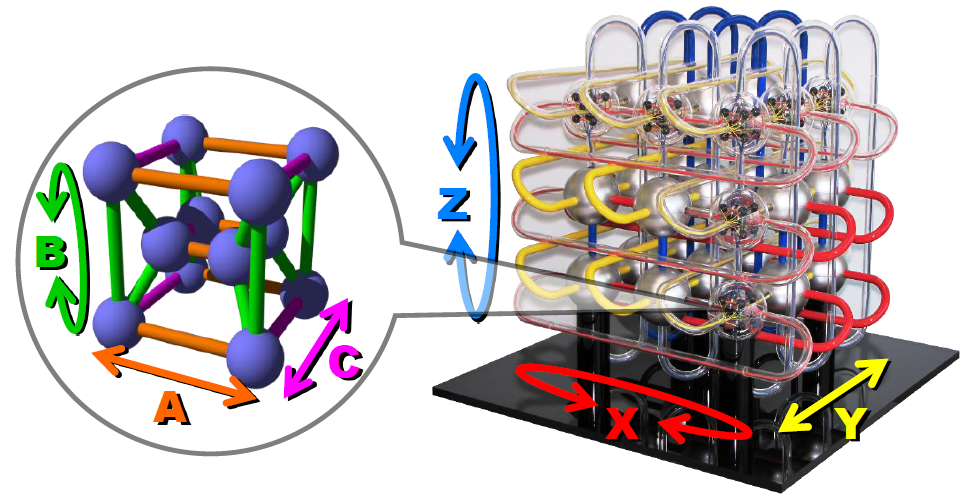
\includegraphics[width=.8\textwidth,height=.4\textwidth]{tofu.png}
\caption{Tofu模块和6D Mesh/Torus结构\upcite{tofu}}
\label{tofuto}
\end{figure}

\subsection{高性能互连网络}

E级高性能计算机系统的研制和应用面临巨大的挑战,
对高性能互连网络来说则面临更大的挑战。
高性能互连网络是高性能计算机系统的重要组成部分,
其主要功能是完成计算节点I/O 节点之间的通信。
随着处理器性能按照摩尔定律提升、
计算系统规模的按照指数级增长,
互连网络越来越成为影响系统性能的主要因素\upcite{johnkim}。
高性能互连网络主要由四个重要部分构成:
拓扑结构,路由算法,拥塞控制以及物理器件。
拓扑结构决定了报文在网络中最短跳步数、
节点间可用的总路径数和二分带宽,
路由算法则决定了报文在网络中的实际跳步数。
物理器件主要指通过拓扑结构相连并封装在机柜内的路由器和物理链路。
实际高性能互连网络通信则是依靠路由算法和拥塞控制机制保证。
除此之外,制约一个高性能互连网络的设计还有
很多因素\upcite{duato2002interconnection}。
主要因素介绍如下:

\textbf{网络性能}消息延迟和网络的吞吐率是网络性能的主要指标。
消息延迟是指消息在源节点开始发送的时间与目的节点接收消息的时间之差。
消息延迟直接影响处理器和存储的使用。
吞吐率则是在单位时间内,网络所能传输最大的信息量。
因为成本开销等原因,网络容量不是一个无底洞,
一旦饱和网络不会再传输新注入的消息,
这严重限制了系统的性能。
这两个指标跟网络拓扑结构的网络直径和链路容量紧密相关。

\textbf{灵活性和扩展性}一个灵活的网络,在扩大或者缩小规模的同时,
相应的带宽需求也按需求按比例增减,以保证性能不降低。
否则,带宽将成为系统瓶颈,降低系统效率。
同时,在物理器件约束下,网络仍然能够支持良好的扩展性,并保证网络性能。

\textbf{应用负载}网络可以根据应用负载的不同将网络中的节点或者链路划分成多个子网,
使得应用负载之间互相不影响性能。
同时,这也是出于安全因素的考虑。

\textbf{物理封装和器件约束}结合实际物理封装因素考虑
如何保持高性能互连网络拓扑本身的优良特性是设计高性能互连网络拓扑的重要问题。
物理封装有两个主要限制影响拓扑设计,一是缆线的长度和数量。
随着光纤技术的发展,机柜内部因为距离较短采用电信号传输,
机柜之间则采用光纤保证长距离的通信质量。
随着系统规模的增大,不仅缆线的数量增加使得物理封装难度增加,
由于机柜数的增加,缆线长度也因此增加而造成网络延迟增加,
如光纤传输延迟为每米5 纳秒。
第二个限制因素则是芯片的带宽和引脚数。
芯片的带宽和引脚数受限于芯片的面积,
在高阶路由器和光纤技术等器件发展不成熟时期,
互连网络受器件约束只能采用节点度数小,
网络直径大的结构,如经典的$k-ary$ $n-cube$结构。
随着工艺的进步,高阶路由器等器件的技术已成熟,
大规模低直径高性能互连网络成为高性能互连网络的主要结构。
除了此之外,简单性和可维护性都跟拓扑设计紧密相关的。
一个好的高性能互连网络拓扑结构一定是易构造,易维护的。

\textbf{可靠性} 为了保证网络性能,高性能互连网络是无损网络,
不支持丢包和重传。
因此,高性能互连网络的可靠性是保证网络传输的重要指标。
一旦发生有错误发生,网络中有多条可选路径保证传输不受影响。
而且,某条链路或者节点发生错误,网络的连通度不受影响等,
都是设计网络结构的时候需要考虑的场景。

\textbf{成本能耗开销} 随着系统规模的增加,
路由器个数和缆线数量的增加,都大大增加了成本和能耗的开销。
尤其,在能耗方面,若是随着规模的增加而线性增长,
将无法完成E 级高性能计算机系统的开发。
因此,在设计网络拓扑结构时,成本能耗开销起着决定性的作用。

\subsection{研究现状和不足}

本节主要回顾国际上在高性能互连网络设计方面的相关工作。
自高性能计算机系统发展以来,在HPCA、ISCA、 SC、 ICS等高性能领域顶级会议上,
高性能互连网络一直都是热点研究方向。
Intel、Cray、IBM、Bull、Mellanox等公司以及
许多研究小组都在关注和致力于研究高性能互连网络,
针对高性能互连网络的拓扑结构设计,路由算法及拥塞控制等方面进行研究。

随着对系统规模的需求增大,以及高阶路由器结构和光纤技术的发展,
大规模高性能互连网络采用低直径拓扑结构成为高性能互连网络的发展趋势。
在高性能计算机系统发展早期,
大部分高性能计算机系统的互连网络采用的要么是树形或者是
$k-ary$ $n-fly$蝶形等间接网络结构,
要么是$k-ary$ $n-cube$直接网络结构。
这些结构的特点都是使用端口数较小的交换机通过多级或者笛卡尔积的方式构建网络。
2007年,Kim等人在ISCA顶级会议上提出了使用高阶路由器搭建大规模
高性能互连网络低直径拓扑结构Flattened Butterfly\upcite{Flattenedbutterfly},
将高阶路由器替代传统的低阶路由器,从而减少路由器数量和降低网络直径。
之后,该组在2008年的ISCA会议上提出新型
高性能互连网络Dragonfly\upcite{dragonfly}结构和
2009年的超级计算机顶级会议SC上提出可灵活配置的HyperX结构\upcite{hyperx},
不仅充分利用高阶路由器的特点还将光纤运用在拓扑结构的不同层次。
至此,使用高阶路由器成为构建高性能互连网络新型拓扑结构的主要手段。
Cray、IBM等大公司也开始使用高阶路由器搭建高性能计算系统,
如Cray公司的Cascade系统\upcite{cascade}和IBM的PERCS系统。

在高性能互连网络拓扑结构方面,
Koibuchi所在的研究小组在2012年的ISCA会议上提出了
使用高阶路由器搭建随机拓扑\upcite{acaserandom},
其不仅网络直径低,平均最短路径小,还可以支持任意的网络规模。
但是,随机拓扑在物理布局中,面临缆线长短不一,连线复杂等不足,
2013年的HPCA会议上他们小组提出layout\-conscious的随机拓扑结构\upcite{fsorandom},
根据实际物理降低缆线的长度减少系统构建的开销。
2015年的HPCA 会议上,他们小组提出在机柜上摆放自由光设备,
根据不同应用的负载,在随机拓扑上添加自由光链路以满足不同的链路需求。
2014年的SC会议上瑞士联邦理工的Besta和Hoefler利用代数图论的方法
构造出近似最优的大规模低直径拓扑Slim Fly\upcite{slimfly}。
Slim Fly结构在不受路由器端口数限制的条件下,相比其他结构,
不仅端口利用率高,而且获得较优的网络性能。
2015年SC会议上Kathareios等人提出一个性价比更高,
直径为2的拓扑结构OFT\upcite{costeffective2}。
在同样的成本开销下,OFT结构相比Slim Fly结构,拥有更好的可扩展性。

高性能互连网络的路由算法是高性能互连网络的研究重点。
一个拓扑即使具备再好的优良特性,
如果没有合适的路由算法也不能展现出优良的网络特性。
路由算法决定了拓扑结构的实际网络性能。
随着系统规模的增加,大规模低直径互连网络成为高性能互连网络的首选。
同时,给设计合适的路由算法带来巨大挑战。
Jiang等人在2009年ISCA会议上对Dragonfly结构提出
间接自适应路由通过本地链路间接反馈来解决全局链路的拥塞\upcite{indirect}。
随后,Garc$\'{\i}$a等人分析出现有的自适应路由算法在解决
Dragonfly结构全局链路拥塞问题的同时引入了本地链路的拥塞,
因此,提出On\-the\-fly路由算法解决全局和本地链路拥塞\upcite{On-the-Fly}的问题。
On\-the\-fly路由算法由于是自适应绕路路由,
如果采用虚通道隔离的方式避免死锁,
路由芯片需要增加虚通道数目而增加缓存资源和控制单元。
不仅会增加了成本开销而且受芯片面积限制。
如果采用逃逸子网的方式避免死锁,
逃逸路径较长会严重影响网络性能。
因此,Garc$\'{\i}$a 等人提出了OFAR-CM\upcite{OFAR-CM}、
RLM\upcite{Rlmolm}和OLM\upcite{Rlmolm}解决On\-the\-fly路由算法的问题,
减少虚通道数量并保证网络性能。
Won等人在2015年HPCA会议上提出了避免
Dragonfly远端拥塞的路由算法\upcite{ofc},
通过添加历史窗口观察正在链路上传输的报文以判断应该走最短路径还是非最短路径。

拥塞控制机制对于高性能互连网络,重要性不低于路由算法。
Kim等人在\upcite{cbcm}中指出,路由算法是解决网络中链路拥塞,
拥塞控制机制则是解决终端拥塞。
路由算法和拥塞控制机制两者密切相关,
相互作用,相互影响,结果都是作用在网络性能上。
传统的Explicit Congestion Notification(ECN)
拥塞控制机制已经广泛使用在高性能互连网络,
如在InfiniBand Architecture\upcite{ecn1}\upcite{ecn2}\upcite{ecn3}。
但是,ECN机制对参数敏感,对拥塞情况反馈时间长,
不能准确及时的对拥塞采取措施。
尤其,高性能互连网络是一个无损网络,不允许网络中有丢包现象,
如果网络中发生拥塞,对网络性能影响巨大。
因此,Kim等人提出的CBCM 策略\upcite{cbcm}针对反馈时间长,
参数敏感等缺点做了有效的改进,
通过引入竞争度的概念,及时监测拥塞并作出反馈。
Jiang等人则提出了预约的方式主动避免终端拥塞\upcite{srp}\upcite{crp}\upcite{lhrp}。
除此之外,还有研究者把解决拥塞的关键放在降低Head-of-Line Blocking(HoLB)
出现概率,如FlexVC\upcite{flexvc}以及Y$\'{e}$benes等人的
相关研究 \upcite{Y2017Providing}\upcite{Y2017An}\upcite{Y2018Head},
有效的利用虚拟通道减少HoLB的发生。

E级计算时代即将到来标志着高性能互连网络也将要进入一个新时代,
但是,这同时也给高性能互连网络现有技术带来了巨大挑战。
目前的高性能互连网络新型拓扑结构无法同时满足E级计算规模、
灵活性、器件约束、物理封装、网络性能、应用负载等需求,
已有的路由算法和拥塞控制机制也随着拓扑规模、
网络直径、 应用负载等变化面临新的挑战。

\section{论文的主要工作}
本文面向高性能互连网络,
针对当前新型高性能互连网络在物理器件约束下如何满足E级计算系统网络规模、
灵活性以及应用负载的需求,路由算法如何解决缓存资源利用率低等问题,
分别对灵活的、满足应用负载的新型高性能互连网络以及
高效利用缓存资源的路由算法等具有挑战性的问题进行深入的研究,
论文的主要工作总结如下:

(1)针对在E级计算的挑战下,
因路由器端口数约束使当前高性能互连网络的灵活性及网络性能方面的不足,
提出一种灵活端口数的高性能互连网络新型拓扑结构Galaxyfly。
Galaxyfly利用代数图论有限域的方法构造而成。
在保持低直径的情况下,Galaxyfly可以达到网络规模和二分带宽的灵活权衡。
其降低了对高阶路由器端口数的要求,
可以使用较少的端口数去构建E级计算系统的网络规模。
针对Galaxyfly结构,不仅分析了可构造的配置并且评估了最短路径数量。
利用其代数图论的性质,设计了拥塞敏感的路由算法。
与其他新型高性能互连网络拓扑结构分别从性能、
成本和能耗三方面进行了实际物理布局的模拟和分析比较。
结果表明Galaxyfly相比其他结构,在不同的路由算法以及典型的通信模式下,
能够展现更优的性能,是一个适合构建E级计算系统的新型高性能互连网络拓扑结构。

(2)针对在E级计算的挑战下,
目前高性能互连网络的网络性能、可维护性以及物理封装方面的不足,
提出一种适合使用多芯光纤的高性能互连网络新型拓扑结构Bundlefly。
Bundlefly是一个低直径、可灵活扩展并且适合采用多芯光纤连接机柜之间的拓扑结构。
随着集成光模块板的发展,一根多芯光纤可以替代一捆传统的单芯光纤,
不仅可以降低光纤的使用成本还可以提高光纤的可维护性。
虽然Bundlefly的网络直径只有3,
但是其不仅能够充分利用多芯光纤来提高机柜间的通信带宽
还能降低高阶路由器的端口数的要求来支持E级系统的可扩展性。
通过分析和模拟,比较了Bundlefly和其他新型高性能互连网络拓扑结构,
Bundlefly能够完成更好的性能。

(3)针对目前高性能互连网络自适应路由算法对虚拟通道数量要求高以及
缓存资源利用均衡的不足,提出了一种标签路由算法Label-based Routing(LBR)。
LBR通过协同设计路由器微体系结构里的输入缓冲区模块和路由计算模块,
将路由计算引入缓冲区模块,
根据网络状态对路由报文做标记。
LBR不仅降低了死锁避免政策对虚拟通道的需求,
还均衡使用缓存资源并有效实现完全自适应路由。
通过模拟在Dragonfly结构上评估了LBR的性能并与其他拓扑结构进行了对比。
实验表明,在大部分通信模式下,LBR优于别的路由算法近10\%-35\%。

\section{论文的组织结构}

本文紧紧围绕高性能互连网络新型拓扑结构和路由算法进行优化设计,
本文共分为六章。
论文组织框图如图\ref{orgth}及各章节主要内容介绍如下:


\begin{figure}[htp]
\centering
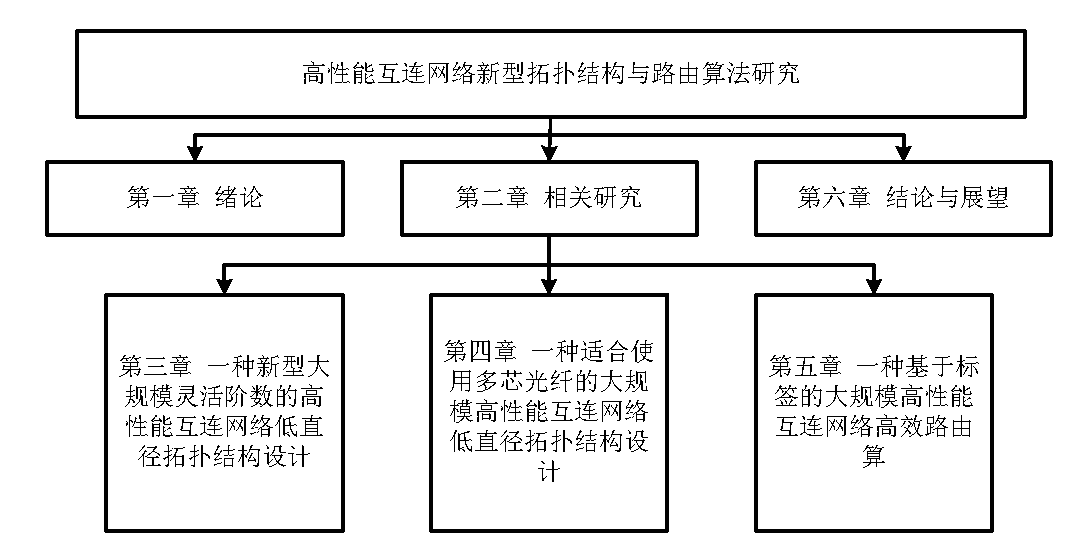
\includegraphics[width=.88\textwidth,height=.45\textwidth]{Visio-org_th.eps}
\caption{论文组织框图}
\label{orgth}
\end{figure}

第一章绪论,首先对高性能计算以及高性能计算机进行介绍,
并论述了高性能互连网络的研究意义以及高性能互连网络设计需要考虑的因素,
然后对高性能互连网络的研究现状以及不足进行分析,
最后简述了本文的主要研究内容和组织结构。

第二章介绍了本文的研究技术背景,包括物理器件对高性能互连网络设计的影响,
高性能互连网络新型拓扑结构,
高性能互连网络路由算法及高性能互连网络拥塞控制机制。

第三章提出了一种灵活端口数的高性能互连网络新型拓扑结构Galaxyfly。
首先详细介绍了Galaxyfly拓扑结构的构造方法,
然后对Galaxyfly结构的灵活性、可构造配置、
最短路径数以及容错性进行了详细的理论分析,
之后描述了Galaxyfly结构的路由算法。
最后通过模拟仿真对Galaxyfly的网络性能进行验证。

第四章提出了一种适合多芯光纤的高性能互连网络新型拓扑结构Bundlefly。
首先详细介绍了Bundlefly拓扑结构的构造方法,
然后对Bundlefly结构的网络直径、可扩展性、二分带宽、最短路径数、平均最短路径
以及容错性进行了详细的理论分析,
之后描述了Bundlefly结构的路由算法。
最后通过模拟仿真对Bundlefly的网络性能进行验证。

第五章提出了一种基于标签的高性能互连网络路由算法Label-based Routing。
首先详细介绍了Label-based Routing算法的整体架构,
然后论述Label-based Routing算法的缓冲区、
路由算法以及虚拟通道分配机制,
最后通过模拟仿真对Label-based Routing的性能进行验证。

第六章结论与展望,对全文的研究内容和主要工作进行总结,并对后续的工作进行展望。

\chapter{相关研究工作}
本章介绍高性能互连网络设计的相关背景知识。
首先介绍了物理器件对新型高性能互连网络的影响,
之后介绍了典型的高性能互连网络拓扑结构和路由算法。

\section{物理器件对高性能互连网络的影响}
传统的高性能互连网络拓扑大致分为两类
,一类是以$k\textrm{-}ary$ $n\textrm{-}fly$蝶形网络为代表的间接网络,
如图\ref{butterfly}所示。
$k\textrm{-}ary$ $n\textrm{-}fly$结构中,节点度数为$2k$,采用单向链路,
网络直径为$n-1$,网络规模为$k^n$。
一类是以$k\textrm{-}ary$ $n\textrm{-}cube$网络为代表的直接网络,
如图\ref{torus} 所示。
$k\textrm{-}ary$ $n\textrm{-}cube$结构中,节点度数为$2n$,采用双向链路,
网络直径为$n \lfloor k/2 \rfloor$,网络规模为$k^n$。
%% FIXME $n(\lfloor\frac{k}{2}\rfloor)$
当$k=2$时,$k\textrm{-}ary$ $n\textrm{-}cube$结构就是经典的超立方体(Hypercube)结构,
是第一代高性能计算机的主要拓扑结构。
如Intel iPSC/2\upcite{ipsc2}、 NCUBE/10\upcite{ncube}、
SGI Origin 2000\upcite{sgi2000} 等系统均采用了Hypercube结构,
因为其具有正则性、对称性、强容错性以及可嵌入性等特点。
当$k=n$时,$k\textrm{-}ary$ $n\textrm{-}fly$结构和$k\textrm{-}ary$ $n\textrm{-}cube$结构规模一样,
节点度数一样,但是$k\textrm{-}ary$ $n\textrm{-}cube$结构的网络直径大约是
$k\textrm{-}ary$ $n\textrm{-}fly$结构的$k/2$倍。
$k\textrm{-}ary$ $n\textrm{-}fly$ 结构拥有更小的网络直径,
但是,路径唯一性及负载不均衡是限制其扩展的主要原因。

%% FIXME annotate these two figures with concreate n/k values?
%% FIXME also more explanation needed in the text?
\begin{figure}[htp]
  \centering
   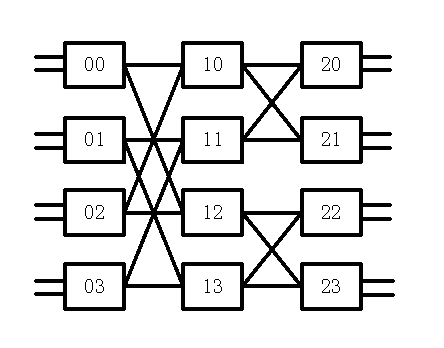
\includegraphics[width=.48\textwidth,height=.38\textwidth]{Visio-butterfly.eps}
    \caption{$k\textrm{-}ary$ $n\textrm{-}fly$结构}
    \label{butterfly}
\end{figure}

\begin{figure}[htp]
  \centering
   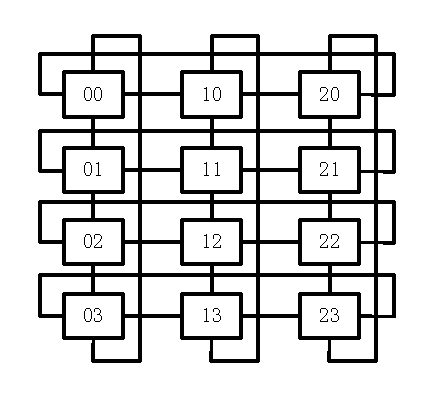
\includegraphics[width=.44\textwidth,height=.38\textwidth]{Visio-torus.eps}
      \caption{$k\textrm{-}ary$ $n\textrm{-}cube$结构}
      \label{torus}
\end{figure}

%% FIXME 10Gb/s or 10GB/s
上世纪90年代,路由芯片引脚带宽上限约为10Gb/s,
%% FIXME 端口数受限是因为引脚带宽低?
路由芯片也因此端口数受限制。
传统的高性能互连网络只能采用低节点度的拓扑结构。
随着半导体和集成电路的发展,路由芯片的引脚带宽增加,芯片端口数也随之增加。
如Cray公司推出的端口数为64的YARC路由芯片
\upcite{yarc}\upcite{blackwindow}、2010年HOTI
会议上提出的48端口Gemini芯片\upcite{cascade}、
2015年HOTI会议上提出48端口的Intel Omni-Path芯片\upcite{omni}以及
Mellanox 公司最新推出的Quantum 200G HDR InfiniBand Switch\upcite{quantum}。
相比拥有较少宽带宽端口的路由芯片,
采用拥有更多窄带宽端口的路由芯片搭建高性能互连网络可以降低网络的延迟和成本开销。
根据Kim的推导,低负载下报文的网络延迟为$T=T_h+T_s=Ht_r+L/b$,
其中$H$是报文的跳步数,$t_r$是每一跳经过路由器的延迟,$L$是报文的长度,
$b$则是链路的带宽。
在规模为$N$的网络中,若使用端口数为$k$的路由芯片($k$个输入通道加$k$个输出通道),
其跳步数最少为$2log_kN$。
若芯片的总带宽为$B$,则$b=B/2k$。
那么网络延迟为$T=2t_rlog_kN+2kL/B$,对$k$求导,
当$dT/dk=0$时可得到网络延迟$T$取最小值时端口数$k$满足$klog^2k=Bt_rlogN/L$。
随着网络规模$N$增加,路由芯片的最佳端口数$k$也随之增加。
%% 不要一句话不停重复地说……
%% 因此,基于高阶路由器设计的高性能互连网络成为高性能互连网络设计的主流趋势。
随着路由器端口数的增加,基于高阶路由器的网络拓扑结构相继被提出,
如Flattened Butterlfy \upcite{Flattenedbutterfly}、Dragonfly \upcite{dragonfly}、
HyperX \upcite{hyperx}等。
相比传统的高性能互连网络拓扑结构,
基于高阶路由器设计的网络拓扑结构不仅可以在降低网络直径的前提下支持更大的网络规模,
还可以减少路由器的数量。
Kim曾预测,未来几年内将会出现数百个端口的路由芯片,
2010年单芯片的总带宽会突破20Tb/s\upcite{yarc}\upcite{blackwindow}。
但是,实际上目前最新的商用芯片总带宽只能达到16Tbps\upcite{quantum}。
总体上,虽然路由芯片取得了长足的发展,
但采用目前的高性能互连网络仍远不足以构建E级计算系统,
如何利用当前商用高阶路由芯片搭建E级计算系统已经成为高性能互连网络研究的关键问题。

光纤技术的发展使得高性能互连网络在实际部署中引入光缆代替部分电缆。
大规模低直径的新型高性能互连网络相比传统的高性能互连网络,
拥有更多的全局链路以降低网络直径。
对全局链路采用光纤部署,不仅在性能上有优势,而且在能耗上独立于榄线的物理长度。
研究表明,10米以内的链路,采用光纤的成本相比电缆的成本要高,
而10米以上的链路,
则采用电缆的成本要比光纤的高\upcite{dragonfly}。
因此,为了降低系统成本,
Dragonfly结构在保证网络直径低的前提下,
每个超级节点只引出一条全局链路连接相邻超级节点\upcite{dragonfly}。
但是,E级计算系统的应用负载复杂多样,
除了对网络结构的局部性有要求外,全局通信将更加频繁,
若只保证超级节点间
只有一条全局链路已不能满足应用负载的需求。
从边缘可插拔光纤收发器到主板集成光模块的转变\upcite{BOA},
多芯光纤(Multicore Fiber)\upcite{MCF}的出现
给高性能互连网络设计带来了新的契机,
这给提升实际部署中机柜间通信带宽提供了更多空间。
多芯光纤,如图\ref{mcf}所示,实际上就是一条光缆里有多个纤芯的光缆,
可以通过分线器分成多个单芯光纤。
一条多芯光纤相比同等纤芯数的一捆单芯光纤,
不仅成本上更加经济,而且维护上更加容易。
因此,如何在高性能互连网络中更好地利用多芯光纤,
有效提升全局通信带宽并保证可扩展性,提高可维护性是构建
E级计算系统的关键问题。

\begin{figure}[htp]
  \centering
    
\includegraphics[width=.48\textwidth,height=.38\textwidth]{Visio-SCF.eps}
    \caption{单芯光纤}
    \label{scf}
\end{figure}

\begin{figure}[htp]
  \centering
    
\includegraphics[width=.48\textwidth,height=.38\textwidth]{Visio-MCF.eps}
      \caption{多芯光纤}
       \label{mcf}
\end{figure}

\section{高性能互连网络拓扑结构}

\subsection{Fat tree}
Fat tree\upcite{fattree}是最早的大规模低直径高性能互连网络拓扑结构。
国防科技大学自主研制的天河一号和天河二号高性能计算机均采用Fat tree结构。
Fat tree是一个灵活性和扩展性都较优的拓扑结构,
最大的特点在于随着网络规模的增加,二分带宽也随之等规模增加。
其可以看成是两个$k\textrm{-}ary$ $n\textrm{-}fly$结构合并而成,
如图\ref{fattree}所示由两个图\ref{butterfly}合并而成,采用双向链路。
%% FIXME use concreate n/k
两个蝶形结构分别起到负载均衡和控制输入输出的作用,
因此,Fat tree继承了蝶形结构网络直径低的优点,
并且可以有效避免蝶形网络路径唯一和负载不均衡等缺点。
Fat tree的节点度数为$2k$,网络直径为$2(n-1)$,
网络规模$2k^n$,且需要$(2n-1)k^{n-1}$个路由器。
%% FIXME 如何用n/k定义胖树?
\begin{figure}[htp]
  \centering
    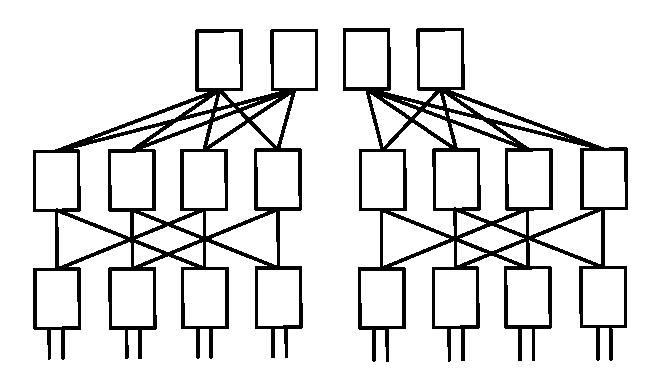
\includegraphics[width=.48\textwidth,height=.38\textwidth]{Visio-fattree.eps}
    \caption{Fat tree结构}
     \label{fattree}
\end{figure}

\subsection{Flattened Butterlfy}

Flattened Butterfly\upcite{Flattenedbutterfly}是2007年Kim等人
在ISCA会议上提出的一个性价比较高的高阶互连网络。
Flattened Butterfly结构充分利用高阶路由器提供的丰富链路特性,
使得$k\textrm{-}ary$ $n\textrm{-}cube$结构中每一维上的路由节点都是全互连,
其节点度为$(n+1)(k-1)+1$,网络直径为$n$,网络规模为$k^{n+1}$。
%% FIXME 如何用n/k定义FB
Flattened Butterfly利用高阶路由器,
不仅有效解决了$k\textrm{-}ary$ $n\textrm{-}cube$结构网络直径长的问题
而且通过合并$k\textrm{-}ary$ $n\textrm{-}fly$结构中的路由器,有效降低了路由器的数量。
如图\ref{flattenedbutterfly}所示,图左是$k\textrm{-}ary$ $n\textrm{-}fly$结构,
图右是合并了蝶形网络中每一层的路由器的Flattened Butterfly。
与Fat tree相比,当搭建同样规模和同样直径的网络时,
Flattened Butterfly可以节省近一半的链路。

\begin{figure}[htp]
  \centering
    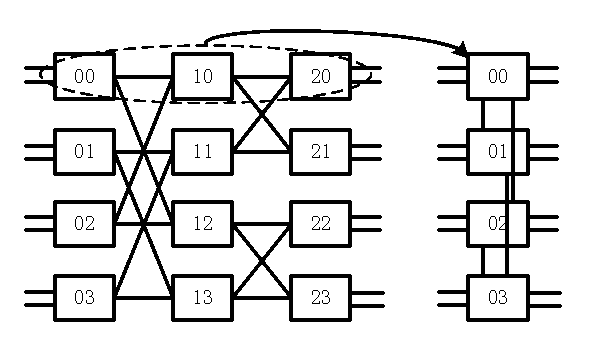
\includegraphics[width=.56\textwidth,height=.35\textwidth]{Visio-flattenedbutterfly.eps}
    \caption{Flattened Butterfly结构}
    \label{flattenedbutterfly}
\end{figure}

2009年SC会议上提出的HyperX\upcite{hyperx}
结构实际上是基于Flattened Butterfly结构的扩展结构,
是一个可以灵活配置的高阶互连网络。
HyperX同样是一个$k\textrm{-}ary$ $n\textrm{-}cube$结构,
但是每一维上的$k$值可以取不同值,
而且每个路由节点所连接的终端数以及每一维上的链路带宽都可以随意配比。
在网络规模、性能需求和能耗成本开销上,
这类可灵活配置的拓扑结构都更适合实际系统的需求。
Hypercube和Flattened Butterfly都是HyperX的特例。

%% FIXME 可能是因为第一章就没有把k-ary n-cube和k-ary n-fly 解释清楚,
%% 后面的拓扑结构感觉都没那么容易理解,以外行的眼光。

\subsection{Dragonfly}

Dragonfly\upcite{dragonfly}结构是一个有标志意义的高阶互连网络,
也是大规模低直经高性能互连网络的典型代表。
相比低阶互连网络,高阶互连网络拥有更多的全局链路,使用更多的长缆线。
为了解决高阶互连网络长缆线成本开销的问题,Dragonfly利用层次化的结构有效
减少了全局链路的数量并同时支持较大的网络规模和较低的网络直径。

Dragonfly具体构造是将$a$个高阶路由器通过全互连的方式相连成虚拟的更高阶超级节点,
每个路由节点引出$a-1$条本地链路连接同一个超级节点内的其他路由节点,
如图\ref{dragonfly}中虚线框所示。每个路由器引出$h$条全局链路
链接其他超级节点内的路由节点。
在全局网络中,虚拟的更高阶超级节点两两之间至少有一条链路相连,
如图\ref{dragonfly}中虚线框之间的连线所示。
通过在不同层次的网络中采用全互连结构,Dragonfly的网络直径只有3。
相比同样规模和同样节点度数的Flattened Butterfly结构,
Dragonfly结构可以节省近一半的全局链路。

\begin{figure}[htp]
  \centering
    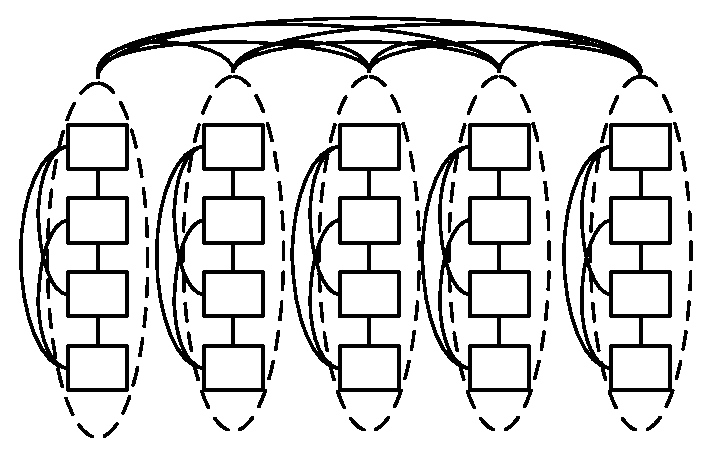
\includegraphics[width=.56\textwidth,height=.35\textwidth]{Visio-dragonfly.eps}
    \caption{Dragonfly结构}
       \label{dragonfly}
\end{figure}

在2017年HiPINEB会议上提出的Dragonfly+\upcite{Dragonfly+}
拓扑结构是在Dragonfly结构的基础上进行扩展优化,
使用直径为2的树形结构替代Dragonfly结构超级节点内的全互连网络,
同时保持网络直径为3,
Dragonfly+使用图\ref{dragonfly+}所示的结构替代图\ref{dragonfly}中的超级节点。
使用相同端口数的路由芯片搭建网络,
Dragonfly+结构可以支持的最大网络规模接近Dragonfly结构的4倍。

\begin{figure}[htp]
  \centering
    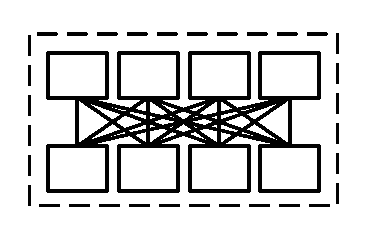
\includegraphics[width=.48\textwidth]{Visio-dragonfly+.eps}
    \caption{Dragonfly+结构中超级节点模块}
    \label{dragonfly+}
\end{figure}

\subsection{Slim Fly}
Slim Fly\upcite{slimfly}是一个近似最优的高性能互连网络拓扑结构。
Slimf Fly的设计目标是,在直径为2的前提下,
使用尽可能少的路由器端口数构造更大规模的拓扑结构。
Slim Fly结构是继Dragonfly结构之后又一个标志性拓扑结构,
其利用代数图论的构造方法,
满足了低直径大规模的要求,
而且在二分带宽和成本能耗以及容错性上都展现了较优的性能。

Slim Fly采用了代数图论里的MMS图\upcite{MMS}。
其构造取决于一个基本参数$q$,$q$是一个素数的幂,可以表示为
$q=4w+\delta$,其中$\delta \in \{-1,0,1\}$。
Slim Fly图是一个高对称性的结构,由两个子图构成,
%% FIXME 每个子图多少子组,每个子组多少节点,用符号表示。
%% 检查以下我理解的对不对,每个子组是不是q个路由节点?
每个子图内包括$q$个子组,每个子组包含$q$个路由节点。
在Slim Fly中,每个路由器引出$q-\delta$条链路连接同一个子组内的其他路由节点,
$q$条链路分别连接另一个子图中$q$个子组的路由节点。
如图\ref{slimflyone}所示,
Slim Fly中的每个路由节点用一个三元组$(a,x,y)$标识,
其中$a\in \{0,1\}$标识子图的编号,
$x,y\in\mathds{F}_q$分别标识在所在子图中子组的编号和
所在子组中路由节点的编号。

令集合$X$和$X'$表示有限域$\mathds{F}_q$的两个生成集\upcite{MMS}\upcite{GRMMS},
他们可以通过有限域$\mathds{F}_q$的生成元$\xi$
通过式\ref{equ:generator-sets0}和\ref{equ:generator-sets1}构造。
那么Slim Fly结构中的链路构造方式如下:
\begin{itemize}
\item 当且仅当$y-y' \in X$,路由节点$(0,x,y)$与路由节点$(0,x,y')$相连。
\item 当且仅当$y-y' \in X'$,路由节点$(1,x,y)$与路由节点$(1,x,y')$相连。
\item 当且仅当$y=x'x+y'$,路由节点$(0,x,y)$与$(1,x',y')$相连。
\end{itemize}

\begin{figure}
  \centering
    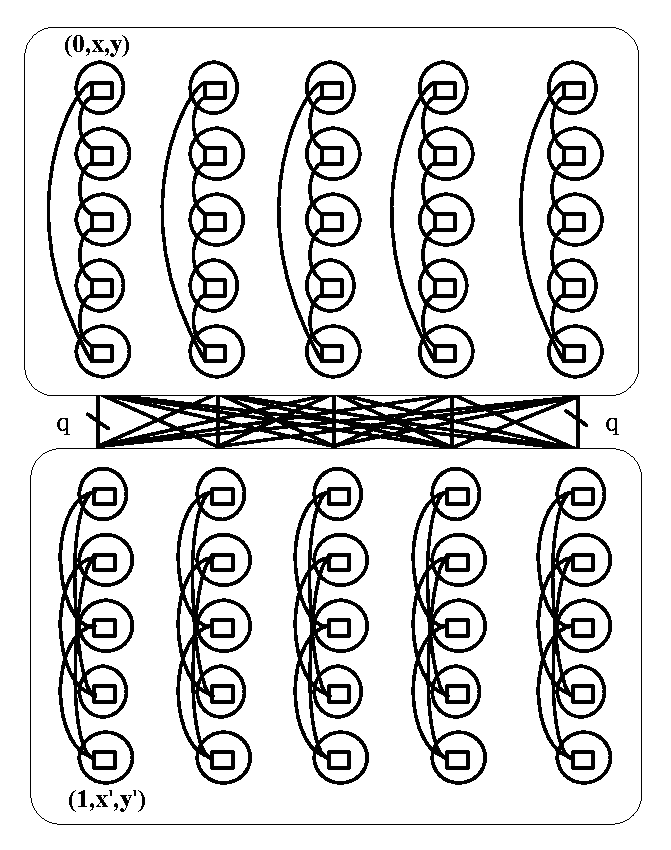
\includegraphics[width=.6\textwidth]{Visio-Slimfly_between.eps}
    \caption{Slim Fly结构}
    \label{slimflyone}
\end{figure}

\begin{equation}\label{equ:generator-sets0}
  X=
  \begin{cases}
    \{1,\xi^2,\ldots,\xi^{q-3}\}& q=4 \ell+1 \\
    \{1,\xi^2,\xi^4,\ldots, \xi^{2\ell-2},\xi^{2\ell-1},\xi^{2\ell+1},\ldots, \xi^{4\ell-3}\} & q=4 \ell-1 \\
    \{1,\xi^2,\ldots,\xi^{4l-2}\} & q=4 \ell
  \end{cases}
\end{equation}
\begin{equation}\label{equ:generator-sets1}
  X'=
  \begin{cases}
    \{\xi,\xi^3,\ldots,\xi^{q-2}\} & q=4 \ell+1 \\
    \{\xi,\xi^3,\xi^5,\ldots,\xi^{2\ell-1}, \xi^{2\ell},\ldots,\xi^{4\ell-4},\xi^{4\ell-2}\}\ \ \ \  & q=4 \ell-1 \\
    \{\xi,\xi^3,\ldots,\xi^{4l-1}\} & q=4 \ell
  \end{cases}
\end{equation}

%% FIXME 上面没说SF的全局网络是什么
在实际物理部署中,Slim Fly可以部署成全局网络是一个全互连网络。
分别位于相邻子图的两个子组封装成一个机柜,
那么任意两个机柜之间都有$2q$条链路,
%% FIXME 这句话在图中也体现不出来
如图\ref{slimfly}所示。

\begin{figure}[htp]
  \centering
    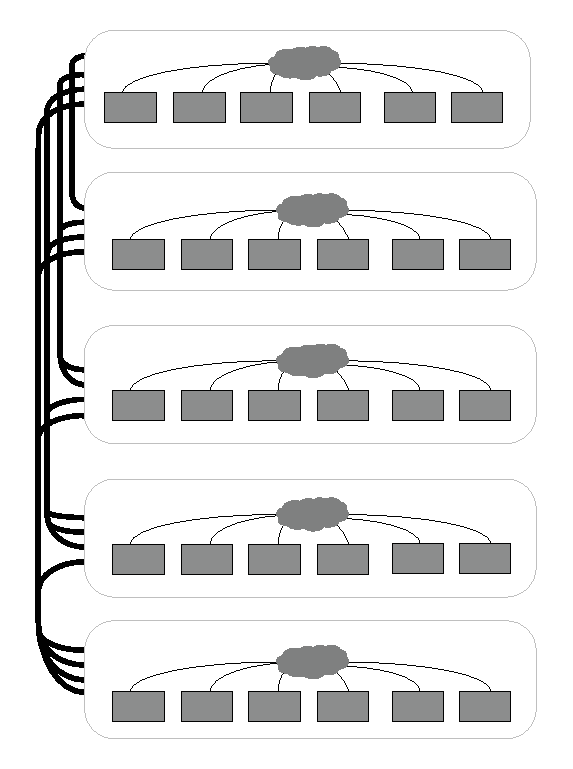
\includegraphics[width=.3\textwidth,height=.5\textwidth]{Visio-Slimfly.eps}
    \caption{Slim Fly结构的全局网络}
    \label{slimfly}
\end{figure}

在2015的SC会议上,两种网络直径为2的间接拓扑结构
OFT(two-level Orthogonal Fat-Trees)和MLFM(Multi-Layer Full-Mesh)
被提出\upcite{costeffective2},
分别如图\ref{oft}和\ref{mlmf} 所示。
在相同条件下,OFT相比Slim Fly和MLMF可以构造近似2倍规模的网络,
MLMF的可扩展性跟Slim Fly一样。
这三种拓扑结构的相同点就是平均每个终端都是消耗3个路由器端口和2条链路。
%% FIXME 这段话仅仅说OFT在规模上更好,但MLFM等于啥都没说。
%% 况且,OFT规模比SF大,那缺点呢?不都是tradeoff么。
%% 再况且,只说如图所是,还应该加一点对图的解释。

\begin{figure}[htp]
  \centering
    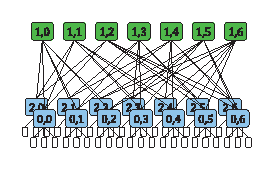
\includegraphics[width=.6\textwidth]{oft.eps}
    \caption{OFT结构\upcite{costeffective2}}
    \label{oft}
\end{figure}

\begin{figure}[htp]
  \centering
    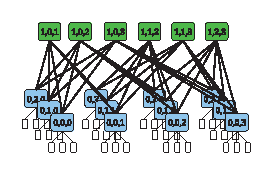
\includegraphics[width=.6\textwidth]{mlmf.eps}
    \caption{MLMF结构\upcite{costeffective2}}
    \label{mlmf}
\end{figure}

\subsection{随机拓扑}

除了前面介绍的规则拓扑外,
随机拓扑也是高性能互连网络新型拓扑结构的一个重要类型。
最早是在数据中心网络中提出使用小世界网络\upcite{smallworld}构造系统。
通过在规则拓扑结构上添加随机链路构造出具有小世界网络特性的随机网络,
图\ref{sw2d}展示了一种在2D Torus结构上添加随机链路构小世界网络形成的拓扑结构。
在约束节点度情况下,具有小世界网络特性的网络
不仅可以拥有较短的网络直径,而且具备较高带宽和较短平均最短路径。
Singla等人提出将Jellyfish\upcite{Jellyfish}
运用在top-of-rack(ToR)交换机之间。
Jellyfish是一个绑定节点度的随机图拓扑结构,
不仅可以支持任意规模,而且相比同样配置的Fat tree,
可以支持更多的节点并提供至少一样的带宽。
Valadarsky等人指出当前最新的拓扑结构,如Slim Fly和Jellyfish,
都是expander图\upcite{xpander}。
但是,在性能上这些拓扑结构还不能达到近似最优,并在它们扩展上和部署上都存在困难。
因此,他们提出Xpander结构\upcite{xpander},不仅提供近似最优的性能,
而且切实提高了部署可行性。
Xpander是一个灵活扩展的拓扑结构,
每个节点表示一个ToR交换机,每个节点有$d$个端口连接其他ToR交换机,
扩展则以包含$d+1$个节点的全互连图为单位进行。
通常情况下,Xpander结构都是通过翻倍的方式扩展,
但是Xpander也支持线性扩展来满足任意规模。
图\ref{xpander}给出了$d=2$的Xpander结构,
即,每个节点有2个端口连接其他节点,
以3个节点的全互连图为单位扩展成节点为6的Xpander结构。
%% FIXME 从这个图上看不出是怎么扩展的,也看不出d表示什么

\begin{figure}[htp]
\centering
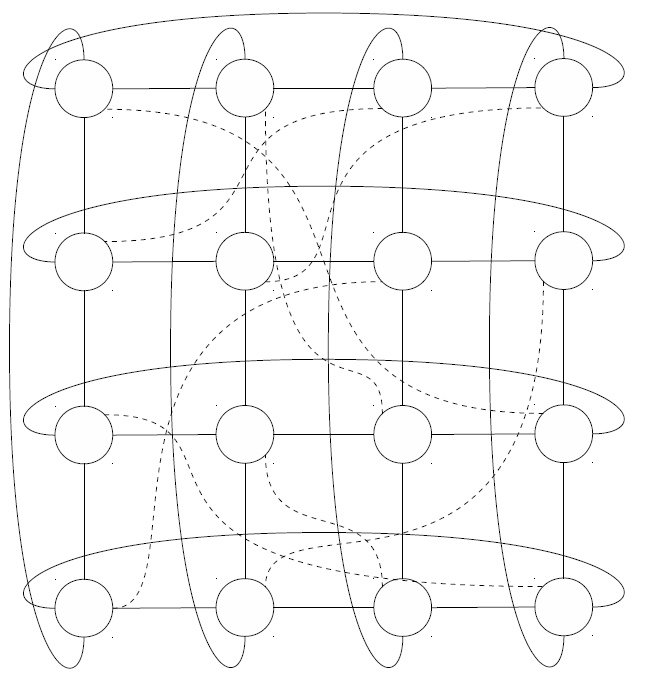
\includegraphics[width=.5\textwidth]{sw2d.png}
\caption{小世界网络\upcite{smallworld}}
\label{sw2d}
\end{figure}
%% FIXME 这个图的线太细了

\begin{figure}[htp]
\centering
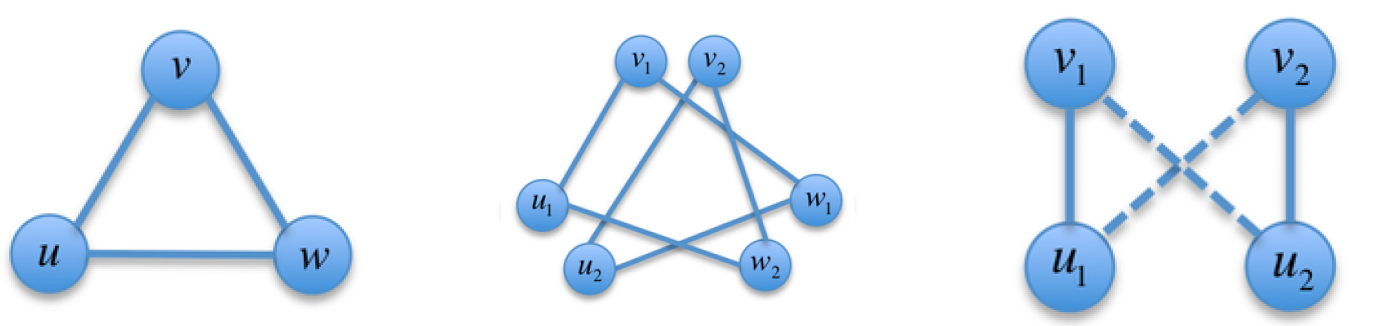
\includegraphics[width=.8\textwidth]{xpander.png}
\caption{Xpander结构\upcite{xpander}}
\label{xpander}
\end{figure}

Koibuchi等人\upcite{acaserandom}首先提出在高性能互连网络中采用随机拓扑结构
以满足系统延迟低、灵活扩展等需求。
具体构造方式类似于小世界网络,在圆环拓扑结构上添加随机链路,
可以支持任意规模的网络。
在2013年的HPCA会议上,
Koibuchi等人在之前提出的随机拓扑上进行了优化\upcite{layoutrandom},
加入了物理布局的考虑,限制了缆线的长度。
之后在2015年的IPDPS会议上他们研究组提出Skywalk拓扑结构\upcite{skywalk},
其进一步约束随机链路在实际物理布局的三维结构中的连接方式
来降低链路延迟对网络延迟的影响。
在2015年的HPCA会议上,
他们研究组提出在机柜间利用基于自由空间光(FSO)的随机链路来
降低网络延迟并优化任务分配\upcite{fsorandom}。
如图\ref{fso}所示,通过在机柜上部署FSO设备,
以便根据任务负载添加FSO通信链路以优化性能。

虽然随机拓扑可以提供较短的网络直径和平均最短路径,
并可以灵活支持任意规模,
但是,路由算法是限制随机拓扑应用于实际系统部署的主要原因之一。
由于随机拓扑结构只能通过路由表的方式进行路由,
随着网络规模的增长,路由表规模呈指数级增长,这是在实践中难以接受的。

\begin{figure}[htp]
\centering
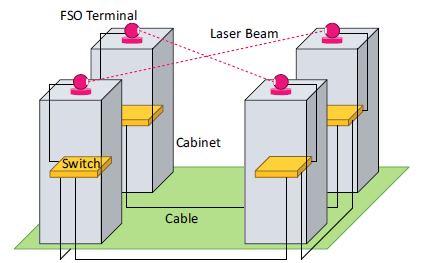
\includegraphics[width=.7\textwidth]{fso.png}
\caption{添加FSO链路的高性能互连网络\upcite{fsorandom}}
\label{fso}
\end{figure}

\section{高性能互连网络路由算法}

拓扑结构和路由算法是紧密相关的,路由算法决定了拓扑结构的实际网络性能。
路由算法除了决定报文在拓扑结构的路径也同时影响网络
在实际通信下的拥塞情况以及网络的死锁避免策略。
虽然在高性能互连网络中,新型拓扑的连接方式多种多样,
但是,相同点都是网络规模大且直径低。
这个相同点造成了新型拓扑结构只有少量的冗余最短路径且部分关键链路使用频率高。
如Slim Fly\upcite{slimfly}结构中只有
极少量的节点对之间的最短路径多于一条,
Dragonfly\upcite{dragonfly}结构中超级节点之间的链路负载很中,容易造成网络的拥塞。
在实际通信中,为了满足不同的应用负载,
使用自适应路由算法是提升网络性能、解决网络中链路拥塞的主要方法之一。
然而,在新型拓扑结构中只能使用非最短路径代替最短路径,
这不仅给自适应路由算法的性能造成影响,
同时也给死锁避免策略带来成本开销和工艺设计等挑战。

Dragonfly结构是高性能互连网络的新型拓扑结构典型代表之一,
学术界针对其结构特点提出了很多路由算法。

最短路径路由(MIN)是Dragonfly结构上最简单和最基本的路由算法\upcite{dragonfly}。
使用最短路径路由最多只需3跳就能将报文从源路由节点传送到目的路由节点,
即:源路由节点所在的超级节点内的本地链路、
源超级节点和目的超级节点的全局链路和目的超级节点的本地链路。
因为Dragonfly的结构特点,本地链路和全局链路的VC可以复用,
因此MIN算法至少需要两条VC来避免死锁。

非最短路径路由又称Valiant路由算法(VAL)\upcite{dragonfly},
是针对高负载流量提出的路由算法。
报文先选择一个中介节点作为第一个目的路由节点,
当通过MIN从源路由节点到达中介节点后再通过MIN 从中介节点到达目的路由节点。
这样做的好处是,缓解高负载流量对全局链路的过度请求。
具体在实施时Valiant路由算法可划分为两种,
一种(VAL)是以中介节点所在的超级节点为第一目的地,
只要报文到达中介节点所在的超级节点就将目的地换成真正的目的路由节点。
第二种(VAL$_n$\upcite{overcomefarend})则是按前面介绍的以中介节点为第一目的地。
第一种VAL最长需要经过5跳到达终点,途
经3条本地链路和2条全局链路。
VAL$_n$则最长需要经过6跳到达终点,途经3条本地链路和3条全局链路。
两种算法都至少需要3条VC来避免死锁。

在均衡随机通信模式下,VAL相比MIN,不仅跳步数翻倍,
吞吐率也会相应减半。而在密集高负载的最差通信模式下,
MIN则会造成全局链路的严重堵塞。
根据网络状态选择走VAL机制或是MIN机制是均衡全局自适应路由算法
(UGAL)的主要机制\upcite{dragonfly}。
网络状态则由路由端口缓冲区队列长度和报文的跳步数共同决定。
由于UGAL最长跳步数由VAL机制决定,
因此,UGAL同VAL一样至少需要3条VC来避免死锁。

上述四种Dragonfly结构路由算法存在一个共同的问题,那就是不能及时感知并反馈全局链路的拥塞状况。
因此,有研究提出间接自适应路由算法\upcite{indirect}来迅速对全局链路的拥塞作出反馈。
图\ref{dragonflyir}展示了四种不同的间接自适应路由算法。
第一种间接自适应路由算法CRT (Credit Round Trip),
通过感知本地链路的信用反馈延迟来判断全局链路拥塞情况使得UGAL算法及时对拥塞做出
反馈,如路由器R0通过本地链路给路由器R1发送报文再通过全局链路给路由器R2发送报文,
路由器R1给路由器R0的信用反馈需等到路由器R2的信用反馈返回到R1才能发送。
CRT通过背压的方式获得全局链路的拥塞信号,
但是可能会造成本地链路拥塞。
第二种间接自适应路由算法PAR(Progressive Adaptive Routing),
如图\ref{dragonflyir}所示,在源超级节点根据当前
拥塞情况作出路由决策,选择MIN或者VAL。
这种方法在发现全局链路拥塞时不会将拥塞情况反馈给源路由器。
该算法会多走一跳本地链路,在使用VC隔离的方法来避免死锁时,需要多一条VC。
PAR可以扩展到在经过的每一个超级节点内部都根据当前网络状态选择MIN或者VAL。
第三种间接路由算法PB(Piggyback),
如图\ref{dragonflyir}所示,
通过给相邻节点广播全局链路的拥塞状态作出路由选择。
具体实现则需要在每个报文上都增加一个记录链路状态的向量位。
每个路由器都需要维护同一个超级节点内全局链路的状态信息。
该算法缺点是路由器需要维护全局链路拥塞信息的更新。
第四种间接路由算法RES(Reservation),
如图\ref{dragonflyir}所示,该方法是报文提前预约全局链路的资源,
如果预约成功则执行MIN路由,不成功则执行VAL路由。
该方法可能会造成预约信息泛滥,并且预约信息可能不及时。

%% FIXME 这个图的问题在于太小了。四个算法应该分成四个子图,最多并排两个,
%% 而且,这个图本身缺乏必要的解释。如,黑色线,橙色线分别什么意义,GC是什么的缩写……
\begin{figure}[htp]
  \centering
    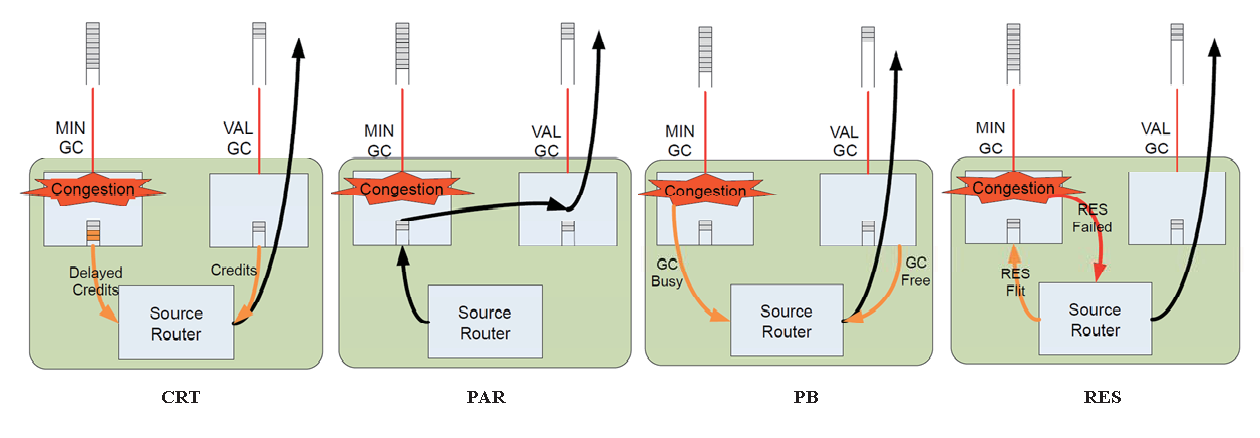
\includegraphics[width=.8\textwidth]{Visio-dragonfly_indirect.eps}
    \caption{Dragonfly结构间接自适应路由算法\upcite{indirect}}
       \label{dragonflyir}
\end{figure}

针对一些特定的通信负载,如最差通信负载,
Dragonfly结构中确定的两个超级节点频繁通信,
不仅会造成全局链路拥塞,还会同时造成本地链路拥塞。
如图\ref{dragonflytr}所示,
在采用了VAL的路由选择后仍然会造成同一个超级节点的
两个路由器因为要转发所连接全局链路传送来的报文导致两个路由器之间的本地链路拥塞。
%% FIXME 结合这个图,上面这句话说的似乎不太明确,我没看懂。
因此,研究者提出On-the-Fly 自适应路由算法(OFAR)\upcite{On-the-Fly}
来解决本地链路和全局链路的拥塞问题。
OFAR通过允许在超级节点内部进行本地链路的绕路,
有效避免了因为全局链路拥塞造成的本地链路的拥塞。
OFAR最长路径长度要达到8跳,如果采用VC隔离的方式避免死锁则至少需要6条VC。
OFAR最初采用的是基于气泡流量控制的哈密尔顿环作为逃逸子网,
OFAR-CM\upcite{OFAR-CM}则在OFAR 的基础上提出拥塞管理机制ECM和BCM,
这两种拥塞控制机制分别关注的是逃逸子网的拥塞情况和正常网络的拥塞情况,
该研究还提出采用树型逃逸子网和up-down路由算法。

\begin{figure}[htp]
  \centering
    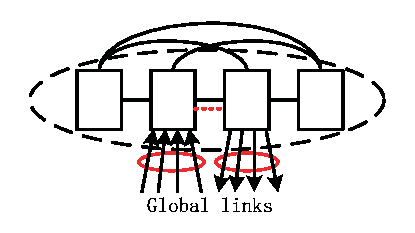
\includegraphics[width=.45\textwidth]{Visio-dragonfly_traffic.eps}
    \caption{Dragonfly结构中全局链路导致本地链路拥塞}
       \label{dragonflytr}
\end{figure}

路由算法中的死锁避免,有多种方法,大致可以分为三类:
一是设计无环路由,二是通过虚拟通道(VC)切换的方式避免死锁,
三是通过逃逸子网的方式避免死锁。
这其中,无环路由是最经济的方法,但是会因限制部分路径不能通行,降低网络吞吐率。
VC 切换的方法的优势是可以充分利用网络中的链路,
但是VC数量的增加给工艺和成本开销带来挑战。
逃逸子网使用一套独立的VC网络或者
物理网络执行一个没有环路的路由算法来避免整个网络的死锁,
相比前两种方法,逃逸子网可以算是一个折中的办法,
但是逃逸子网的使用频率影响网络性能。
RLM 和OLM算法\upcite{Rlmolm}的提出有效降低了OFAR对VC的需求。
RLM在超级节点内部采用转弯模型的方式避免死锁,即超级节点内部采用无环路由,
通过减少路径多样性降低VC数量。
OLM则是采用限制VC使用顺序的方式避免死锁,
利用VC降序作为逃逸路径,
在保证超级节点内的路径多样性的同时不额外增加VC数量。

除了考虑不同的通信负载和拓扑结构的特征,
也要考虑实际物理布局中缆线长短对路由算法决策的影响。
在\upcite{overcomefarend}中指出目前大多数
已有的工作都没有考虑远端延迟的影响,即下几跳后的网络拥塞和因路由器之间
较长链路延迟高引起的拥塞,实际上这些拥塞都只是暂时性的拥塞,
不会导致网络真正拥塞。
比如,较长的链路延迟会使得一些报文或者信用不能及时到达终点从而造成拥塞的假象。
因此,作者通过历史窗口的方法来避免这种假象影响自适应路由的决策
\upcite{overcomefarend}。

另外,是否能够合理分配缓冲区资源也是路由算法的性能的影响因素。
Gorgues等人\upcite{Achieving}提出在$k\textrm{-}ary$ $n\textrm{-}cube$结构的片上网络上,
通过报文标记的方法给报文均衡分配网络中的缓冲区资源并利用更少的资源来避免死锁。
具体设计是每个输入端口有2条VC,
每条VC被分配一个报文长度的缓冲区大小。
完全自适应路由算法通过通过一条逃逸路径来避免死锁。
每次路由决策都可能改变报文的标记,
如果报文的决策是按维序路由算法路由的话就被标记为安全报文。
否则,则被标记为不安全报文。
每个端口的两条VC中至少有一条VC里全是安全报文或者为空。
我们考虑将这种方法运用在片间网络上,不仅可以避免工艺上的挑战又能充分利用网络资源。

Head-of-Line Blocking(HoLB)问题也是影响路由算法性能的重要因素。
HoLB问题是指位于队列头的报文因为下一级拥塞不能前进阻挡了队列中其他报文前进。
相比确定性路由算法,即在源节点已经确定好报文传输路径,
自适应路由算法因为路由的灵活性会造成报文传输路径不唯一,
更容易造成HoLB问题\upcite{holbara}。
有研究组针对不同拓扑结构路由算法的HoLB问题提出了解决办法。
如在\upcite{holbara}中,针对直接网络的自适应路由算法,
利用有限的VC,将不同目的节点的报文分配到不同的VC中传输。
在\upcite{bbq}\upcite{DBBM}\upcite{iodet}中,
都使用类似的方法解决HoLB问题。
另外,提出上述方法的研究组也针对Dragonfly结构、Slim Fly结构
等典型新型高性能互连网络拓扑结构的路由算法提出了HoLB问题的解决方案
\upcite{holbdf}\upcite{holbsf}。
在FlexVC\upcite{flexvc}中则是提出一个缓冲区管理策略来降低网络HoLB问题,
具体方法就是在保证无死锁的前提下,
尽可能的增大VC可选择的范围。
如针对Slim Fly结构,如果采用最短路径路由算法,
网络中有3条VC的时候,报文就可以选择Opportunistic路径进行路由来降低HoLB问题。

\section{高性能互连网络拥塞控制机制}
拥塞控制机制与路由算法是影响高性能互连网络网络性能的重要因素。
自适应路由算法旨在解决网络中的链路拥塞问题,
而拥塞控制机制则是解决终端节点的超额订购。
当两者搭配使用才能更好的提升网络性能。
%% FIXME 把这句话从后面移到此处,是否使得后面CBCM的表述不清楚?

由于高性能互连网络具备无损的特性,即不会因为网络拥塞而丢包,
传统的拥塞控制机制,如TCP协议,就不适用于高性能互连网络。
高性能互连网络中经典的拥塞控制机制,
如Explicit Congestion Notification(ECN)拥塞控制机制,
是一种被动的拥塞控制机制,根据缓冲队列长度,
给报文打标签,到达目的节点后将拥塞信息通过ACK报文告诉源节点。
这种策略最大的缺点就是不能及时对拥塞作出反馈,响应速度慢。
在2012年的SC会议上,Jiang等人提出
Speculative Reservation Protocol (SRP)\upcite{srp}拥塞控制机制。
SRP是一种主动拥塞控制机制,
通过light-weight的终端预约机制以及投机报文传输机制有效缓解热点通信模式下的拥塞,
获得比ECN机制更高的吞吐率。
之后,该研究组在2013 年SC会议上提出
Channel Reservation Protocol(CRP)\upcite{crp}策略,
专门解决大规模无损网络通信中关键链路拥塞的问题。
因为考虑到成本和技术的限制,集群之间的链路都是供小于求,
如图\ref{crp}所示,如果热点H不能正常吸收负载则会造成
数据流Z拥塞在点A,进而产生拥塞树,
不仅影响集群0的数据流Y还影响集群1内要到达点H的数据流。
CRP通过预约关键链路的方法来解决瓶颈链路拥塞的问题。
在2015年的SC会议上,
该研究组针对ECN和SRP对small message终端拥塞反应速度慢和易造成
拥塞树等不足,
提出Small-Message SRP(SMSRP)和
Last-Hop Reservation Protocol (LHRP)两种策略\upcite{smsrp}。
相较于SRP策略,
SMSRP策略会在发送预约报文之前发送一些投机报文以免造成带宽浪费
以及因为预约产生的动荡。
LHRP相较于SRP和SMSRP策略的不同之处是在最后一跳交换机处根据终端的缓冲队列长度对
投机报文传输失败作出反馈。

\begin{figure}[htp]
  \centering
    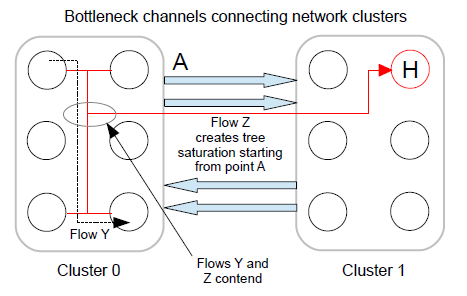
\includegraphics[width=.65\textwidth]{crp.png}
    \caption{集群间的拥塞树\upcite{crp}}
       \label{crp}
\end{figure}

除了上述基于预约的拥塞控制机制,Kim等人在2016年的MICRO会议上
提出一种新的拥塞管理策略Contention-based Congestion Management(CBCM)
\upcite{cbcm}。该研究指出,当网络中只采用自适应路由算法来提升网络性能的时候,
往往会造成拥塞扩散性能降低的情况。
CBCM的原理如图\ref{cbcm}所示,CBCM专门使用一条额外的VC分离终端拥塞的影响,
一旦发现终端拥塞,即终端接收到被标记的报文超过阈值,
则节流相应的源节点,且节流的报文在此额外的VC中采用最短路由算法,
从而避免因为自适应路由算法扩散拥塞。

\begin{figure}[htp]
  \centering
    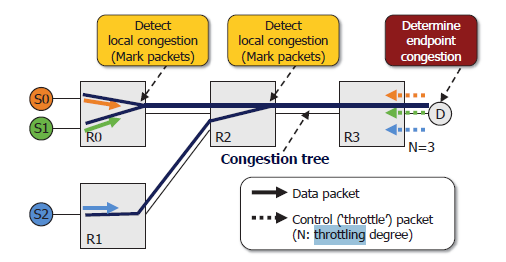
\includegraphics[width=.65\textwidth]{cbcm.png}
    \caption{Contention-based Congestion Management机制\upcite{cbcm}}
       \label{cbcm}
\end{figure}
%\section{模拟环境和性能测试平台}

\section{本章小结}
本章主要阐述了大规模低直径高性能互连网络的理论基础和相关研究。
主要综述了目前已提出的典型高性能互连网络的拓扑结构和典型路由算法、拥塞控制机制等内容。
%% 本文基于大规模低直径的特点开展高性能互连网络拓扑结构设计和路由算法的研究。

\chapter{Galaxyfly:一种灵活可配置的低直径拓扑结构设计}

\section{引言}
当前,大规模高性能计算机系统已经达到数万个计算节点的规模,
如“神威$\cdot$太湖之光”系统和天河二号系统。
高性能计算机系统规模仍然在增长,预计2023年将推出的E级系统,
规模将达到几十万计算节点。
互连网络对高性能计算机系统的扩展能力起到决定性作用,影响着整个系统的设计。
而拓扑结构设计又是互连网络设计中最重要的部分,
因为拓扑结构决定了网络的理论性能上限(如端到端的延迟和二分带宽)与成本开销。

为下一代大规模高性能计算机设计一个有效的拓扑结构需要考虑几个指标。
第一,高带宽和低延迟一直是优化网络拓扑结构的重要目标。
第二,尽可能降低成本开销与功耗开销,
研究表明,互连网络的成本开销和功耗开销分别能够达到整个系统开销的
$33\%$\upcite{Flattenedbutterfly} 和$50\%$\upcite{Energy}。
而E级系统的功耗需要限制在20-30MW以内\upcite{nextplatform}。
最后一点,灵活性也是一个有效拓扑结构的重要指标,
这里的灵活性指拓扑结构在一个以应用为主的高性能计算系统设计\upcite{Reconfigurable}中,
可以通过静态布局或者动态配置成为适应不同应用和通信需求的互连网络。

当前大多数研究的关注点集中在设计低直径的拓扑结构,
同时优化成本和其他指标。一些优秀的低直径拓扑结构相继被提出,
如Flattened Butterfly\upcite{Flattenedbutterfly}、Dragonfly\upcite{dragonfly}、
HyperX\upcite{hyperx}、Skywalk\upcite{skywalk} 和Slim Fly\upcite{slimfly}。
这些拓扑结构虽然能够提供较低的网络直径,
但在规模扩展能力方面,仍不足以支持E级甚至规模更大的高性能计算系统。
限制这些拓扑结构扩展性的主要因素是路由器端口数不足。
进一步增加路由器端口数以支持当前高阶拓扑结构达到E级系统规模对当前乃至未来几年的
商用路由器设计都是十分困难的。
芯片的物理资源和功耗开销是两个限制端口数增长的重要因素\upcite{roleoptics}。
48端口的路由器\upcite{omni}是当前最新的商用模块,
并计划应用在Argonne实验室、
Cray公司以及Intel公司联合推出的180Pflops的高性能计算机系统中。
很多研究者针对这些挑战提出了若干高阶路由器模型,
如64端口的基于瓦片的YARC交换机\upcite{blackwindow}、
64端口的2D Swizzle-switch\upcite{swizzle}、
64 端口的3D Hi-Rise交换机\upcite{hirise}和136端口的SCOC交换机\upcite{scoc}。
但是,这些设计距离应用到实际系统中还需很长的一段时间。
比如说,SCOC的每个端口的速率为25Gbps\upcite{scoc},
略低于现在的商用路由器,
如Intel公司的48端口Omni-Path交换芯片和Mellanox公司的36端口EDR InfiniBand交换芯片。
随着节点计算能力的增长,要维持均衡网络(保持bytes-to-flops的比例),
计算节点链路的链路带宽也要与计算能力按比例增长。
%% 而且,bytes-to-flops的比例关系到每个节点的网络通信总量和浮点运算能力,
%% 这是均衡网络的重要标志。一个计算节点的链路带宽随着计算能力而有比例的增加。
为了满足前沿网络的需求,网络传输速率已经开始采用200Gbps的技术\upcite{road200G}。
当前最先进的200G交换芯片是由Mellanox公司推出的HDR InfiniBand交换芯片,
但也只有40 个端口\upcite{quantum}。

增加高阶路由芯片端口数的同时增加端口带宽是非常困难的,
这是因为在电信号路由器芯片上,增加端口数的同时维持或增加每个端口的带宽
要受到交换crossbar的连线复杂度、芯片边缘的带宽密度\upcite{roleoptics}
以及高速SerDes的I/O的严格限制。
硅光子技术被期望来解决这些困难。
Altera和Avago已经设计出一种基于嵌入并行光模块的光信号FPGA\upcite{avagotech}。
但是,在一块芯片上集成容纳足够的光模块仍然是很困难的工作。
端口数增加的同时也会增加芯片的功耗开销。
例如,在天河二号计算系统中一条SerDes 链路传输一个比特需要消耗20pJ,
而且SerDes的功耗开销占一个芯片的总开销的$79\%$\upcite{Liao2015}。
而且,物理封装设计面积和热量的限制将要严重影响高速SerDes
的数量以及路由器端口数的密度\upcite{road200G}。
因此,E级互连网络设计将要面对路由器端口数影响扩展性的问题。

大多数已有的工作都是关注高阶拓扑结构,
如Fat tree、Flattened Butterfly\upcite{Flattenedbutterfly}、Dragonfly\upcite{dragonfly}、
HyperX\upcite{hyperx}、Skywalk\upcite{skywalk} 和Slim Fly\upcite{slimfly}等。
高阶拓扑结构相比低阶拓扑结构(如:Torus和Mesh结构)可以获得更低的网络延迟。
Fat tree是一个经典的高阶间接网络,
可以通过增加层数使用较低阶的路由器搭建大规模网络,
但是这样会消耗大量链路和路由器。Dragonfly结构不仅网络直径低,
而且结合了光链路和电链路的优势减少网络开销。
但是,使用当前最新推出的商用高阶路由芯片
(如:48端口的Intel Omni-Path 交换芯片\upcite{omni})
来构建Dragonfly网络,其规模仍然不能达到100K。
实际上,Dragonfly结构的扩展性问题限制了他在实际系统中的部署。
比如,Cray公司的Cascade系统\upcite{cascade}采用的是变形的Dragonfly结构,
为了增强结构的可扩展性,
组内结构不是标准定义的全互连结构而是2维的Flattened Butterlfy 结构。
Dragonfly+\upcite{Dragonfly+}被提出来扩展传统Dragonfly结构,
它使用树型结构代替超级节点内的全互连结构并且支持相近的性能。
使用相同端口数的路由器,Dragonfly+的规模可以达到Dragonfly规模的数倍。
在给定的网络规模指标下,Dragonfly+使用的路由器端口数可以减半但是路由器数量翻倍。
HyperX 可以灵活调整参数配置,是一个灵活的拓扑结构。
其每一维上是一个全互连的结构,非常适合使用光链路互连。
Flattened Butterfly 和Hypercube都是HyperX 结构的特例。
但是,HyperX的最大问题就是每一维上全互连的结构会大大影响网络的扩展和增加网络的开销。
随机拓扑结构\upcite{acaserandom}\upcite{layoutrandom}\upcite{Jellyfish}
提供了不一样的设计空间和满足递增式的扩展,
无论网络规模有多大、路由器端口数有多少,都可以构造出来。
然而,随机拓扑结构的路由算法和链路拥塞是随机拓扑结构的最大问题。
Slim Fly基于有限域相关理论构造出一个近似Moore bound规模的网络。
Slim Fly的设计初衷是在给定节点度数和网络直径为2的条件下构造尽可能大规模的网络。
然而,Slim Fly的扩展性受限制于他的低延迟和路由器端口数。
在当前路由器端口数不可能快速增加的情况下,
我们不得不重新权衡节点度和网络直径,即网络性能和网络可扩展性
对高阶拓扑结构设计的影响。

除了这些高性能计算系统的拓扑结构,数据中心系统的拓扑结构也值得高性能计算系统借鉴。
Xpander\upcite{xpander}是最近提出的接近随机网络性能的规则结构。
Xpander可以递增的扩展并可以很好的管理缆线。
但是,Xpander结构内的连线是不确定的,
仍然面临路由表规模大的问题。
Dcell\upcite{dcell}和Bcube\upcite{bcube}都是层次化网络。
Dcell是一个迭代结构而且随着节点度的增加规模呈指数倍扩展。
Bcube是一个以终端为中心的网络结构即终端的网卡接口数增加网络规模增加。
因此,Dcell 和Bcube不能很好的支持灵活扩展。
一些可配置的网络结构被提出通过增加自由光链路\upcite{fso}
或者无线链路\upcite{FireFly}来满足不同应用和扩展性的需求。
但是,这种拓扑构建的设备成本和环境要求高于别的拓扑结构。

本章的目标是设计一种拓扑结构,支持使用现有的商用路由器构建
E级计算系统规模的高性能互连网络。
此外,在设计过程中将灵活性作为重要的设计目标,
使得该拓扑结构可以通过参数配置灵活调整网络规模和二分带宽,
支持部署从P级到E级,甚至更大规模的高性能互连网络。
在前述设计目标下,我们提出了一类新型低直径拓扑结构,Galaxyfly。
Galaxyfly的核心思想是在维持一个较小的网络直径的前提下,在网络规模和二分带宽之间做合理折中。
Galaxyfly基于代数图论有限域的方法构建,
特殊的代数性质使得该拓扑结构
(1)降低了对高阶路由器端口数的要求,
(2)允许通过配置若干个参数支持不同的网络规模,
(3)便于设计延迟敏感的路由算法。
Galaxyfly是一个灵活的层次化拓扑结构,
以Galaxy图和全互连图分别作为全局网络与局部网络。
这种层次化的结构设计可以很好的利用芯片间光互连和背板之间的互连技术,
并易于物理布局,也使得Galaxyfly能够更好地适应不同的通信模式,
如局部的全互连适用局部的密集通信以及全局的冗余链路可以自适应地平衡全局通信负载。
Galaxyfly是一个通用的拓扑结构,Dragonfly和全互连结构都可以看作
Galaxyfly在特定参数配置下的特例。

本章的主要贡献如下:

\begin{itemize}
\item 我们提出了一种新的图结构,Galaxy图,Galaxy图的直径最多为2。
  在Galaxy图的基础上,定义了Galaxyfly拓扑结构。
\item 我们分析了Galaxyfly的结构特性,在灵活性、二分带宽、最短路径数与容错性等方面
  与其他高阶低直径拓扑结构进行了对比分析。
\item 为Galaxyfly拓扑结构设计了最短路径路由算法和
  其他非最短自适应路由算法。
\item 比较了Galaxyfly的不同配置下与其他拓扑结构在物理布局下的性能。
  相比其他经典拓扑结构,Galaxyfly因为灵活的物理布局特性减少了成本开销和功耗开销。
\end{itemize}

\section{Galaxyfly拓扑结构}

本节描述Galaxyfly拓扑结构的构造方法与结构特性。
首先介绍Galaxy图的结构,然后基于Galaxy图与全连通图构造完整的Galaxyfly拓扑。

\subsection{Galaxy图}

本小节将将介绍Galaxy图的构造过程,并证明Galaxy图的直径最多为2。

Galaxy图是一个规模为$nq$的图$G(V,E)$,
其所有节点均匀地划分为$n$个集群$V= V_{0}\cup V_{1}\cup \cdots \cup V_{n-1}$,
每个集群包含$q$个节点,$q$是一个素数幂且可以表示为
$q=4\ell+\delta$,其中$\delta\in\{-1,0,1\}$。
Galaxy图中的链路分为两类,分别是
(1)集群内链路,连接同一集群内的节点,
(2)集群间链路,连接分属不同集群的节点。
在本节后续内容中,我们将分别介绍集群内链路与集群间链路的构造过程。
为便于理解,构造过程将使用一个$n=3$,$q=5$的实例。

\subsubsection{集群内链路}
在给出Galaxy图集群内链路的构造过程之前,
这里先给出若干必要的代数图论与有限域的相关背景知识。
本文只列出一些基本结论,更多的理论细节可以参考文献\upcite{Geometric}。
%% 相关概念里所有的算术操作都需要进行模$q$的运算。

Galaxy图中每一个集群包含$q$个节点。
$q=4\ell+\delta$,$\delta\in\{-1,0,1\}$是一个素数幂,
那么$q$产生一个有限域$\mathds{F}_q=\{x_{0},x_{1},...,x_{q-1}\}$。
%% 其中,$\mathds{F}_q^+$是他的加法群。
在有限域$\mathds{F}_q$中,存在一个生成元$\xi \in \mathds{F}_q$,
使得$\mathds{F}_q$可以通过$\mathds{F}_q = \{\xi^t \bmod q | t \in \mathds{N}\}$的形式生成。
给定有限域$\mathds{F}_q$及其生成元$\xi$,
通过$\xi$可以构造出两个生成集$X$和$X'$,
构造方式分别如式\eqref{equ:generator-sets0}与\eqref{equ:generator-sets1}所示。
易知,两个生成集$X$和$X'$大小相同,$|X|=|X'|=(q-\delta)/2$,
且$\mathds{F}_q = X \cup X' \cup \{0\}$。

\begin{equation}\label{equ:generator-sets0}
  X=
  \begin{cases}
    \{1,\xi^2,\ldots,\xi^{q-3}\}& q=4 \ell+1 \\
    \{1,\xi^2,\xi^4,\ldots, \xi^{2\ell-2},\xi^{2\ell-1},\xi^{2\ell+1},\ldots, \xi^{4\ell-3}\} & q=4 \ell-1 \\
    \{1,\xi^2,\ldots,\xi^{4l-2}\} & q=4 \ell
  \end{cases}
\end{equation}

\begin{equation}\label{equ:generator-sets1}
  X'=
  \begin{cases}
    \{\xi,\xi^3,\ldots,\xi^{q-2}\} & q=4 \ell+1 \\
    \{\xi,\xi^3,\xi^5,\ldots,\xi^{2\ell-1}, \xi^{2\ell},\ldots,\xi^{4\ell-4},\xi^{4\ell-2}\}\ \ \ \  & q=4 \ell-1 \\
    \{\xi,\xi^3,\ldots,\xi^{4l-1}\} & q=4 \ell
  \end{cases}
\end{equation}

基于前述有限域、生成元与生成集的概念,我们给出生成图的定义:
\begin{definition}\label{def:generator-graph}
  若$q$为素数幂,
  $\mathds{F}_q$是$q$的有限域且$\xi$是其生成元,
  $X$,$X'$是生成元$\xi$构造的生成集。
  令$\hat{X} \in \{X, X'\}$表示任一生成集,
  那么$\hat{X}$的生成图$\hat{G}=(\hat{V}, \hat{E})$
  是一个规模为$q$的图,其节点集为$\hat{V} = \mathds{F}_q = \{x_{0}, x_{1}, \cdots, x_{q-1}\}$,
  边集为$\hat{E} = \{(x_i, x_j)\ |\ (x_i - x_j) \bmod q \in \hat{X}\}$。
\end{definition}

对于Galaxy图中的每一个集群,它的内部的结构都可以看作是$X$的生成图。
也就是说,集群内链路的构造规则为:先将集群内$q$个节点分别赋予编号
$\{x_{0}, x_{1}, \cdots, x_{q-1}\}$,节点$x_i$与$x_j$中存在链路
当且仅当$(x_i - x_j) \bmod q \in X$。

\paragraph{例} 在$n=3$,$q=5$的Galaxy图中,$q=4\ell+\delta=5$是一个素数幂,
其中$\ell=1 \in \mathds{N}$,$\delta=1 \in \{-1,0,1\}$。
$q$的有限域为$\mathds{F}_q = \{0,1,2,3,4\}$,
生成元为$\xi = 2$。
根据式\eqref{equ:generator-sets0}与\eqref{equ:generator-sets1},
可以构造生成集$X=\{1,4\}$ and $X'=\{2,3\}$,
根据生成图的定义\ref{def:generator-graph},
可以按照X的生成图构造出Galaxy图中三个集群的集群内链路,如图\ref{hfunction2}。

\subsubsection{集群间链路}

集群间链路由一个同构函数$H$决定。
我们首先给出一个有关同构图的引理,
然后再给出同构函数$H$的定义。

\begin{lemma}\label{thm:generator-graph}
  令$q$为素数幂,
  $\mathds{F}_q$是$q$的有限域且$\xi$是其生成元,
  $X$,$X'$是生成元$\xi$构造的生成集。
  若$G$,$G'$分别是$X$,$X'$的生成图,
  则$G$ 和$G'$是同构图\upcite{Geometric}。
\end{lemma}

基于引理\ref{thm:generator-graph},同构函数$H$定义如下:
\begin{definition}\label{def:isomorphic-function}
  同构函数$H$是一个定义在
  $\mathds{F}_q = \{x_{0}, x_{1}, \cdots, x_{q-1}\}$上的一对一函数,
  对于$\forall x_i \in \mathds{F}_q$,$H(x_i) = x_j$当且仅当
  生成图$G$中的节点$x_i$与生成图$G'$中的节点$x_j$是同构关系中的对应节点。
\end{definition}

根据定义\ref{def:generator-graph}和\ref{def:isomorphic-function},
可以得到以下关于同构函数$H$的引理:
\begin{lemma}\label{thm:isomorphic-function}
  令$q$为素数幂,
  $\mathds{F}_q$是$q$的有限域且$\xi$是其生成元,
  $X$,$X'$是生成元$\xi$构造的生成集,
  $G$,$G'$分别是$X$,$X'$的生成图。
  若$H$是定义在$\mathds{F}_q$上基于$G$,$G'$的同构函数,
  那么对于任意$x_i, x_j \in \mathds{F}_q$,
  $x_i - x_j \in X$当且仅当$H(x_i) - H(x_j) \in X'$。
\end{lemma}

因为$G$,$G'$是同构图,在$\mathds{F}_q$必定存在一个同构函数$H$。
给定同构函数$H$,Galaxy图中任意两个集群$V_s$,$V_t$($0 \leq s < t < n$)
之间的集群间链路可以通过下列方式构造:
对$V_t$中的每一个节点$x_i$($i = 0, 1, \cdots, q-1$),
将$x_i$连接到$V_s$中的节点$H(x_i)$。

\paragraph{例}
图\ref{hfunction0}左半部分展示了生成集$X=\{1,4\}$和$X'=\{2,3\}$
的生成图$G$和$G'$,
根据$G$和$G'$的同构关系,可以找到一个同构函数$H$
$H(0) = 0$, $H(1) = 2$, $H(2) = 4$, $H(3) = 1$, $H(4) = 3$。
集群$V_0$、$V_1$与$V_2$两两之间的集群间链路可以通过
该函数构造。
图\ref{hfunction0}右半部分展示了集群$V_0$与$V_1$之间的链路。
图\ref{hfunction1}展示了$n=3$,$q=5$的Galaxy图的完整结构。

\begin{figure}[htp]
  \centering
  \begin{minipage}[t]{\textwidth}
    \centering
    \subfloat[集群内链路]{
      \includegraphics[height=.30\textwidth]{intra}
      %% 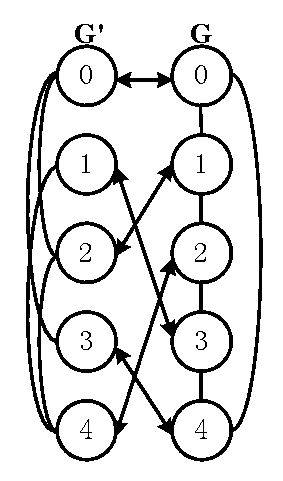
\includegraphics[width=.20\textwidth,height=.38\textwidth]{Visio-intercluster0.eps}
      \label{hfunction2}
    }
    \hspace{.5cm}
    \subfloat[集群间链路]{
      \includegraphics[height=.30\textwidth]{gg}
      %% 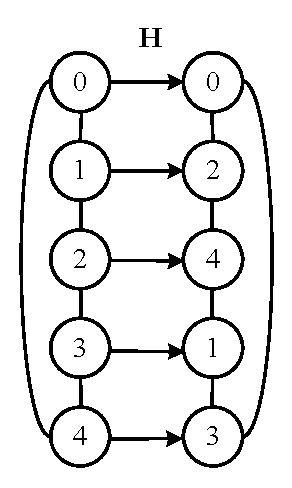
\includegraphics[width=.20\textwidth,height=.38\textwidth]{Visio-intercluster1.eps}
      \label{hfunction0}
    }
    \hspace{.5cm}
    \subfloat[完整结构]{
      \includegraphics[height=.30\textwidth]{edges}
      %% 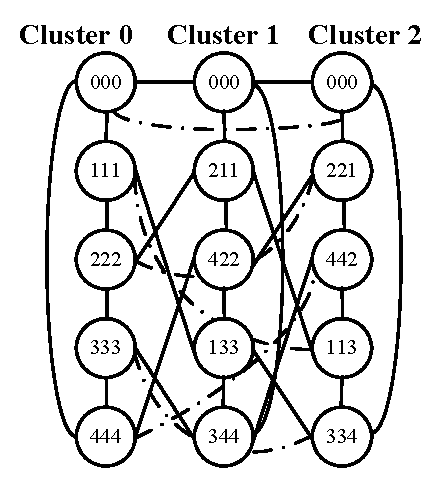
\includegraphics[width=.34\textwidth,height=.38\textwidth]{Visio-Hfunction1.eps}
      \label{hfunction1}
    }
    \caption{Galaxy图($n=3$,$q=5$)}
    \label{hfunction}
  \end{minipage}
\end{figure}

\subsubsection{Galaxy图网络直径}

关于Galaxy图的网络直径,有如下定理:
\begin{theorem}
\label{proofgalaxygraph}
Galaxy图的网络直径最多为2。
\end{theorem}

\begin{proof}

当$q=1$时,Galaxy图是一个全互连图,直径为1。

当$q>1$时,考虑Galaxy图中任意两个节点$n_i$、$n_j$,
它们的标号分别为$x_i$、$x_j$($x_i, x_j \in \mathds{F}_q$)。
可以分两种情况讨论:

(1)$n_i$、$n_j$属于同一个集群。
令$m = x_i - x_j$,如果$m \in X$ ,那么根据集群间链路构造规则,
在节点$n_i$与$n_j$之间存在一条链路,
$n_i$与$n_j$之间的最短路径长度为1。
如果$m \notin X$,$n_i$与$n_j$没有直接相连。
由于$n_i$与$n_j$都有$(q-\delta)/2$条链路连接
到同一集群内的其他节点,
那么从$n_i$与$n_j$出发,共有$q-\delta$条集群间链路
连接到其他$q-2$个节点。
因为$q-\delta > q-2$对于$\delta \in \{-1,0,1\}$恒成立,
所以节点$n_i$、$n_j$在集群内必定存在共同的邻节点,
此时$n_i$与$n_j$之间的最短路径长度为2。

(2)$n_i$、$n_j$属于不同的集群。
不失一般性地,假设$n_i \in V_s$,  $n_j \in V_t$,其中 $s < t$。
令$m = x_i - H(x_j) \bmod q$。
因为$m \in \mathds{F}_q$且$\mathds{F}_q = X \cup X' \cup \{0\}$,
又可以分为三种情况讨论:
(a) $m = 0$,此时由集群间链路构造规则可知,$n_i$与$n_j$之间存在一根链路,
$n_i$与$n_j$之间的最短路径长度为1。
(b) $m \in X$,那么集群$V_s$中标号为$H(x_j)$的节点
是$n_i$与$n_j$的共同邻节点,
此时$n_i$与$n_j$之间的最短路径长度为2。
(c) $m \in X'$,那么根据引理\ref{thm:isomorphic-function},
有$H^{-1}(x_i) - x_j \in X$,
也就是说,集群$V_t$中标号为$H^{-1}(x_i)$的节点
是$n_i$与$n_j$的共同邻节点,
此时$n_i$与$n_j$之间的最短路径长度为2。

综上所述,Galaxy图中任意一对节点之间最多2跳可达,即Galaxy图的直径为2。

\end{proof}

\subsection{拓扑构造}

%% Galaxyfly是一类低直径拓扑结构并由Galaxy图和全互连图组成。
%% 其使用端口数受限制的商用路由器也能满足可扩展性的需求。
%% Galaxyfly也是一个灵活的层次化结构,不仅可以较好
%% 的匹配高性能计算应用的通信模式特征,而且可以通过
%% 调整拓扑结构的参数配置和二分带宽以满足本地通信和
%% 全局通信。在表\ref{Table1}中介绍了Galaxyfly使用
%% 的参数表格。

将Galaxy图中的每一个节点替换成由$a$个路由器组成的超级节点,
超级节点内部$a$个路由器全互连,这样就得到了Galaxyfly拓扑结构。

Galaxyfly由5个基本参数$(n,q,a,p,h)$定义,表示为GF$(n,q,a,p,h)$。
表\ref{tab:gfparams}列出了这些基本参数的具体含义,
而表\ref{tab:gfderivedparams}列出了论文中使用到的其他符号的含义。
可以看出,GF$(n,q,a,p,h)$的基本结构如下:
整个网络由$n$个集群组成,
每个集群包含$q$个超级节点,
每个超级节点包含$a$个路由节点,
共计$N_r=nqa$个路由节点。
每个路由节点连接$p$个终端,
因此网络规模为$N=nqap$。

\begin{table}
  \centering
  \caption{Galaxyfly拓扑结构的基本参数}
  \label{tab:gfparams}
  \begin{tabular}{l l}
    \toprule
    参数 & 描述 \\
    \midrule
    $n$	& 网络中集群的数目\\
    $q$	& 单个集群中超级节点的数目\\
    $a$	& 单个超级节点中路由节点的数目\\
    $p$	& 单个路由节点连接终端的链路数目\\
    $h$ & 单个路由节点连接其他超级节点的链路数目\\
    \bottomrule
  \end{tabular}
\end{table}

\begin{table}
  \centering
  \caption{Galaxyfly拓扑结构的其他参数}
  \label{tab:gfderivedparams}
  \begin{tabular}{lll}
    \toprule
    参数 & 表达式   & 描述 \\
    \midrule
    $N_r$& $nqa$    & 网络中路由节点总数 \\
    $N$  & $nqap$   & 网络中终端总数(网络规模) \\
    $r$  &          & 路由器端口数\\
    $g$  & $a-1$    & 单个路由节点连接所在超级节点其他路由节点的链路数目\\
    $l_t$& $ap$     & 单个超级节点连接终端的链路数目\\
    $l_s$& $ah$     & 单个超级节点连接其他超级节点的链路数目\\
    $h_g$& $n-1$    & 单个超级节点连接其他集群超级节点的链路数目\\
    $h_s$& $(q-\delta)/2$ & 单个超级节点连接所在集群其他超级节点的链路数目\\
    \bottomrule
  \end{tabular}
\end{table}

具体到每个路由器,有$p$条链路连接到终端,
$g$条链路连接到同个超级节点内的其他路由器,
$h$条链路连接到其他超级节点内的路由器。
由于超级节点内部$a$个路由器全互连,因此$g=a-1$。
令$r$表示路由器的端口数,那么拓扑GF$(n,q,q,p,h)$
必须满足约束(\ref{gfcons0}),即路由器的链路总数不超过其端口数。

如果将超级节点看作一个虚拟结点,
那么该虚拟结点有$l_t=ap$条链路连接终端,$l_s=ah$条链路连接其他超级节点。
而根据Galaxy图的构造过程,$l_s$条连接其他超级节点的链路中,
至少要有$h_s=(q-\delta)/2$条链路通往所在集群其他超级节点与
$h_g=n-1$条链路通往其他集群的超级节点,共计$n-1+(q-\delta)/2$条链路,
因此由$l_s \ge h_g + h_s$我们得到GF$(n,q,q,p,h)$必须满足的另一个约束(\ref{gfcons1})。

\begin{equation}\label{gfcons0}
  r \ge p+(a-1)+h
\end{equation}
\begin{equation}\label{gfcons1}
  ah \ge n-1+(q-\delta)/2
\end{equation}

%% 一般情况,超级节点内部的链路和超级节点之间的链路分别是本地链路和全局链路。
%% 根据超级节点规模$a$的大小,我们可以设置集群内和集群之间的链路为本地链路
%% 和全局链路。超级节点和集群的概念类似于Dragonfly结构里超级节点和Slim Fly结构
%% 里子组的概念。

Galaxyfly拓扑中超级节点的概念与Dragonfly中的超级节点、Slim Fly中的子组相似。
层次化的网络结构使得Galaxyfly可以很好地适应不同HPC应用程序的流量特征。
通过调整参数$(n,q,a,p,h)$,
Galaxyfly可以在网络规模与二分带宽之间做灵活的折中
以适应不同种类的流量模式,如增大$a$以增加本地链路的比例适应以本地流量为主的应用。

\begin{table}
  \centering
  \caption{Galaxyfly参数配置示例}
  \label{tab:gfexample}
  \begin{tabular}{lcl}
    \toprule
    参数配置 & 网络直径 & 描述 \\
    \midrule
    GF$(n\!\!=\!\!1,q\!\!=\!\!1,a\!\!>\!\!1,p,h)$ & 1 & 全连通图\\
    GF$(n\!\!>\!\!1,q\!\!=\!\!1,a\!\!=\!\!1,p,h)$ & 1 & 全连通图\\
    GF$(n\!\!>\!\!1,q\!\!>\!\!1,a\!\!=\!\!1,p,h)$ & 2 & Galaxy图\\
    GF$(n\!\!>\!\!1,q\!\!=\!\!1,a\!\!>\!\!1,p,h)$ & 3 & Dragonfly结构\\
    GF$(n\!\!>\!\!1,q\!\!>\!\!1,a\!\!>\!\!1,p,h)$ & 5 & 通用Galaxyfly结构\\
    \bottomrule
  \end{tabular}
\end{table}

\paragraph{例}
Galaxyfly是一种高阶低直径的拓扑结构,
通过调整几个基本参数$(n,q,q,p,h)$可以搭建不同的互连网络。
表\ref{tab:gfexample}给出了一些例子。
其中GF$(n=1,q=1,a>1,p,h)$和GF$(n>1,q=1,a=1,p,h)$是全连通图,直径为1。
图\ref{largeGF0}展示了GF$(n>1,q>1,a=1,p,h)$的结构,
该配置实际就是Galaxy图,直径为2,它与Slim Fly类似,
可以看成一个扁平的网络,没有本地和全局的区别。
图\ref{largeGF1}展示了GF$(n>1,q=1,a>1,p,h)$的结构,
该配置本质上就是Dragonfly结构,即Dragonfly可以看作Galaxyfly的一个特例,其直径为3。
最后,GF$(n>1,q>1,a>1,p,h)$是通用Galaxyfly结构,直径为5,参见图\ref{largeGF2}。
事实上,Galaxyfly的网络直径上限为5。

\begin{figure}[t]
  \centering
    \begin{minipage}[t]{\textwidth}
   \centering
   \subfloat[GF($n>1,q>1,a=1,p,h$)]{
  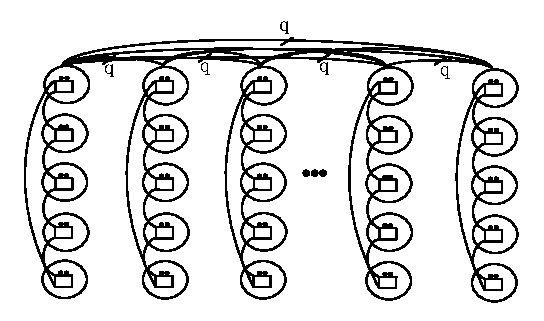
\includegraphics[width=.45\textwidth,height=.30\textwidth]{Visio-largeGF2.eps}
  \label{largeGF0}
  }
   \subfloat[GF($n>1,q=1,a>1,p,h$)]{
  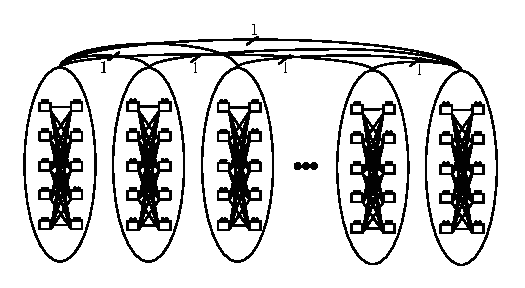
\includegraphics[width=.45\textwidth,height=.30\textwidth]{Visio-largeGF1.eps}
  \label{largeGF1}
  }

   \subfloat[GF($n>1,q>1,a>1,p,h$)]{
  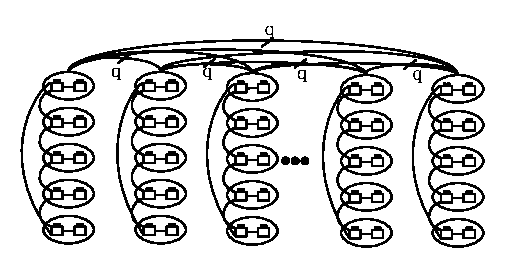
\includegraphics[width=.45\textwidth,height=.30\textwidth]{Visio-largeGF0.eps}
  \label{largeGF2}
  }
  \caption{Galaxyfly}
  \label{gfgraph}
    \end{minipage}
\end{figure}

\section{Galaxyfly结构分析}

在这一节中,我们分析Galaxyfly结构特征,包括灵活性,二分带宽,
最短路径和容错性。我们将Galaxyfly(GF)与其他典型拓扑结构,
如Dragonfly(DF)\upcite{dragonfly}、Flattened Butterfly(FB)\upcite{Flattenedbutterfly}、
Fat tree(FT)和Slim Fly(SF)\upcite{slimfly}进行对比分析。
在后续部分中,我们将使用缩写表示上述拓扑结构。

\subsection{灵活性}

灵活性是指一个拓扑结构构建不同规模的网络的能力,
一个灵活的拓扑结构允许通过调整参数支持构建从P级到E级甚至更大规模的高性能计算系统。
灵活性是一个高效的拓扑结构必须具备的属性。
在限定路由器端口数$r$的前提下,
我们通过比较不同拓扑支持搭建的网络规模范围来比较拓扑的灵活性。
%% 一种是使用一样端口数的路由器构造不同规模的网络。另一种则是使用不同端口数的路由器
%% 构造同一规模的网络。

通过调整参数$(n,q,a,p,h)$,GF可以用来搭建不同规模的互连网络。
使用48端口路由器,图\ref{fig:Figure4}描述了GF拓扑结构在不同参数配置下,
网络规模$N$与路由器连接终端数目$p$的关系。
在图\ref{fig:Figure4}中,我们选取了表\ref{tab:gfexample}中列出的配置,
其中网络直径为1、2、3的配置分别绘制在图\ref{fig:Figure40}、\ref{fig:Figure41}、\ref{fig:Figure42}中,
网络直径为5的配置绘制在图\ref{fig:Figure43}与\ref{fig:Figure44}中。
从图\ref{fig:Figure4}可以看出GF的规模可以从小于1K扩展至超过10000K。
其基本规律是,所选配置的网络直径越大,该配置可以支持的最大网络规模越大。
因此,GF其参数配置的实质是在网络规模和网络直径之间做折中。
最后,图\ref{fig:Figure43}和图\ref{fig:Figure44}展现了$a$的不同取值是如何影响网络规模的,
随着$a$的增大,可以构建的网络规模也随之增大。

\begin{figure}[t]
  \centering
  \begin{minipage}[t]{\textwidth}
   \centering
   \subfloat[GF$(n\!\!>\!\!1,q\!\!=\!\!1,a\!\!=\!\!1,p,h)$]{
  \includegraphics[width=.32\textwidth]{gfscale_a}
   \label{fig:Figure40}
  }
   \subfloat[GF$(n\!\!>\!\!1,q\!\!>\!\!1,a\!\!=\!\!1,p,h)$]{
  \includegraphics[width=.32\textwidth]{gfscale_b}
   \label{fig:Figure41}
  }
   \subfloat[GF$(n\!\!>\!\!1,q\!\!=\!\!1,a\!\!>\!\!1,p,h)$]{
  \includegraphics[width=.32\textwidth]{gfscale_c}
 \label{fig:Figure42}
  }\\
     \subfloat[ GF$(n\!\!>\!\!1,q\!\!=\!\!n,a\!\!>\!\!1,p,h)$]{
  \includegraphics[width=.32\textwidth]{gfscale_d}
 \label{fig:Figure43}
  }
     \subfloat[ GF$(n\!\!>\!\!1,q\!\!=\!\!n,a\!\!>\!\!1,p,h)$]{
  \includegraphics[width=.32\textwidth]{gfscale_e}
   \label{fig:Figure44}
  }

   \caption{不同配置下Galaxyfly的扩展性(使用48端口路由器)}
  \label{fig:Figure4}
  \end{minipage}
\end{figure}

图\ref{fig:Figure3}比较了GF与其他拓扑的灵活性。
其中,选取的FB与FT拓扑结构分别为3维FB与3层FT。
DF作为GF的一个特例,其本身可以通过调整参数$a$、$p$和$h$
来支持不同的网络规模,
但由于DF的最大规模以及均衡配置是在满足$a = 2p = 2h$的条件下取得,
因此在这里我们选取了该最佳配置。
对于GF,我们选取了$GF(n>1,q=n,a=2,p,h)$和$GF(n>1,q=n,a=3,p,h)$。
从图\ref{fig:Figure3}中可以看出,在给定端口数的条件下,
与其他拓扑结构相比,GF$(n>1,q=n,a=3,p,h)$可以构建出规模最大的互连网络,
同时可构建的网络规模范围也最大,即灵活性最高。
SF的优势在于,在指定节点度与严格限定网络直径为2的情况下,可以构建的网络规模最大,
然而,如果只限定路由器端口数,SF可以构造出的网络规模范围最小,灵活性最差。
尽管FT可以通过增加层数将规模扩展至100K,但需要使用大量的线缆与路由器,
成本开销过大且部署难度也会迅速提高。
DF是除GF外扩展性最佳的网络,优于FB与FT,
但在限定路由器端口为48的情况下,仍然无法搭建出100K的网络。

\begin{figure}[t]
  \centering
  \includegraphics[width=2.5in]{cmpscale}\\
  \caption{不同拓扑结构的扩展性(使用48端口路由器)}
  \label{fig:Figure3}
\end{figure}

%% 灵活性同时也表现在一个拓扑在同样规模下能用多少不同的路由端口数路由器构建。换句话说就是,不同的商用路由器能够被用来构造要求的网络规模。没有
%% 对路由器的限制。特别是GF结构,同一规模能够被不同的配置使用不同范围的
%% 端口数的路由器搭建网络。随着网络直径的增加,可构建要求规模的路由器端口数
%% 范围越大,而且在大部分情况下支持的最小端口数则越低。

\subsection{二分带宽}
一般地,在设计互连网络时要给定目标网络的规模$\bar{N}$。
对Galaxyfly而言,选取的参数$(n,q,a,p,h)$必须使得网络规模达到目标规模,
如式(\ref{gfcons2})所示。
\begin{equation}\label{gfcons2}
  nqap \ge \bar{N}
\end{equation}

可行配置不仅要网络规模的要求,还要满足二分带宽的要求。
二分带宽是所有网络平均二分中最小切割的带宽,是评价拓扑结构性能的传统指标。
我们假设每条链路的带宽为1,那么网络的最小二分切割$C_{min}$就等于二分带宽。
在均衡随机通信负载下,只要图的二分最小切割有$N/4$条双向链路就使网络是均衡负载的,
于是我们得到Galaxyfly设计的一个性能约束,$C_{min} \ge N/4$。
由于非堵塞拓扑结构要求至少有$N/2$条双向链路通过图的最小二分切割,
令$\beta=C_{min}/(N/2)$,那么$C_{min} \ge N/4$可以等价地表示为式(\ref{gfcons3})。
\begin{equation}\label{gfcons3}
  \beta \ge 0.5
\end{equation}

至此,我们得到了Galaxyfly的可行参数配置空间,
该空间为约束(\ref{gfcons0})--(\ref{gfcons3})构成的集合。

令端口数上限$r \le 48$(当前商用高阶路由器端口数),
图\ref{chap03figure6}展示了在可行参数配置空间中找到的
$\beta \approx 0.5$的Galaxyfly配置的网络规模。
我们选取SF、3D FB、5D FB作为对比,将他们的网络规模也绘制在图\ref{chap03figure6}中。
由于GF和SF的不规则性,这两种拓扑结构的二分带宽无简单的解析表示。
因此对于GF和SF,我们使用图划分工具METIS\upcite{METIS}近似求解它们的二分带宽。
我们按照网络直径分组,同一张图中展示出的拓扑机构具有相同的网络直径。

\begin{figure}[t]
  \centering
  \begin{minipage}[t]{\textwidth}
    \centering
    \subfloat[网络直径$D=2$]{
      \includegraphics[width=.4\textwidth]{bbw_sf_a}
      %% 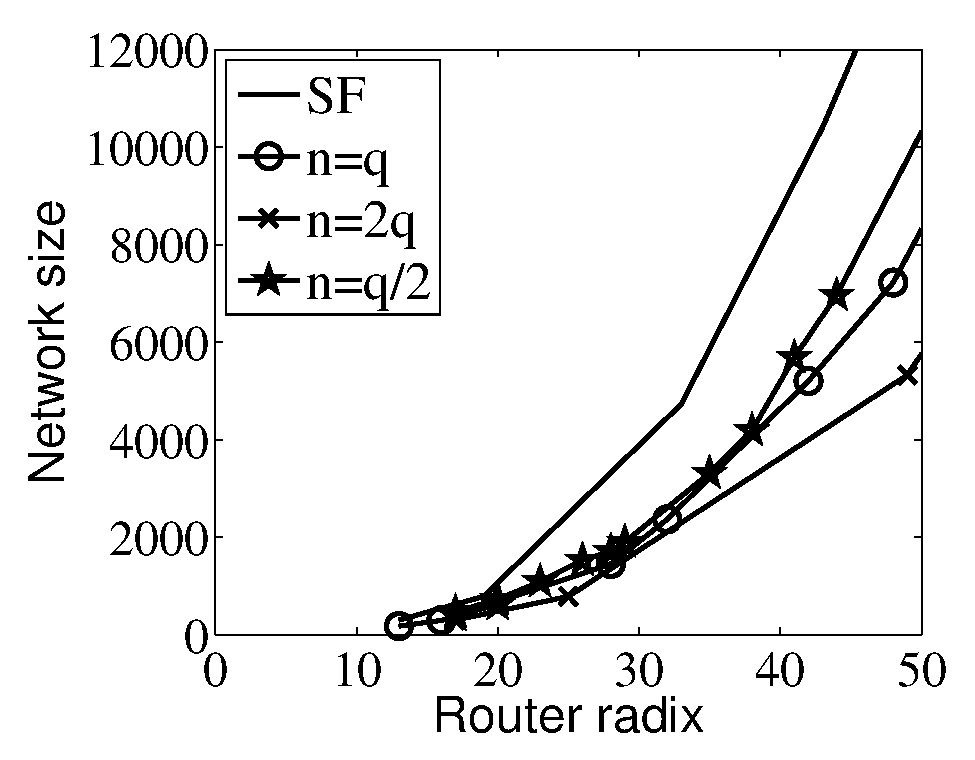
\includegraphics[width=.4\textwidth]{BB_1_v11.eps}
      \label{fig:bbw_sf_a}
    }
    \subfloat[网络直径$D=2$]{
      \includegraphics[width=.4\textwidth]{bbw_sf_b}
      %% 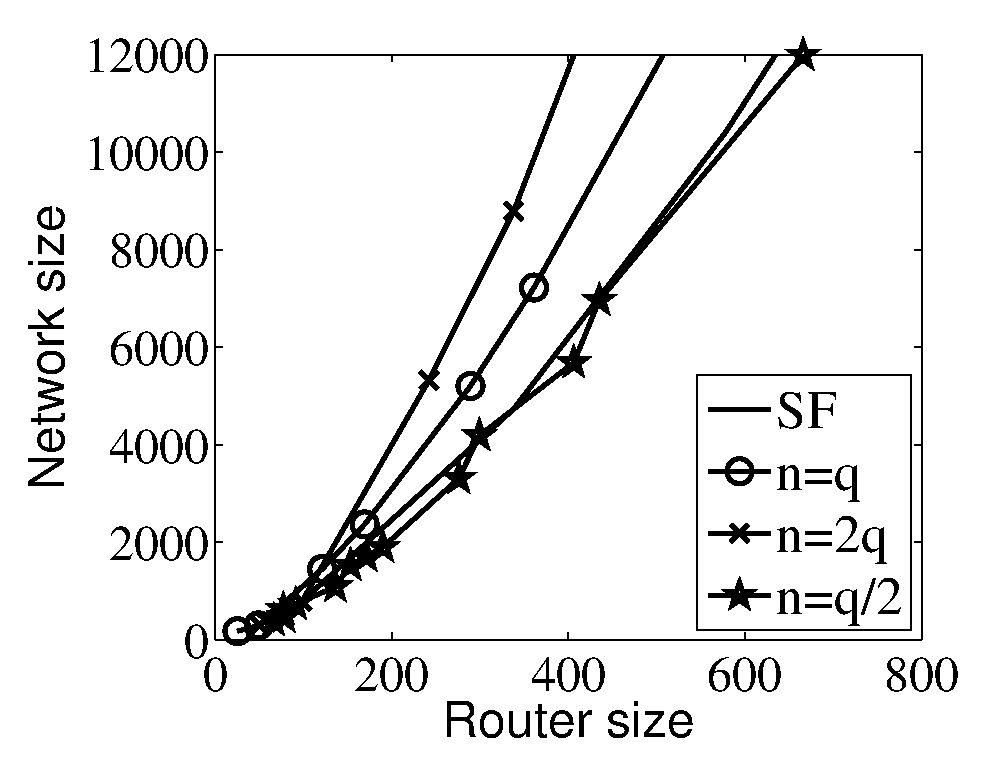
\includegraphics[width=.4\textwidth]{BB_1_v12.eps}
      \label{fig:bbw_sf_b}
    }
    \\
    \subfloat[网络直径$D=3$]{
      \includegraphics[width=.4\textwidth]{bbw_3dfb_a}
      %% 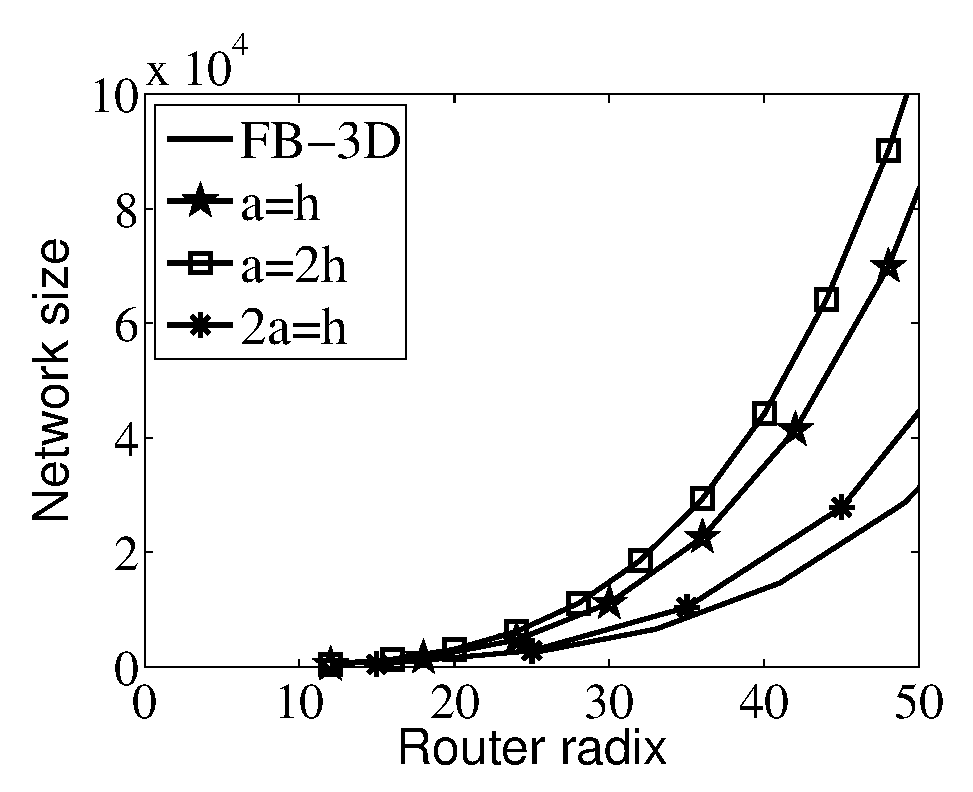
\includegraphics[width=.4\textwidth]{BB_1_v13.eps}
      \label{fig:bbw_3dfb_a}
    }
    \subfloat[网络直径$D=3$]{
      \includegraphics[width=.4\textwidth]{bbw_3dfb_b}
      %% 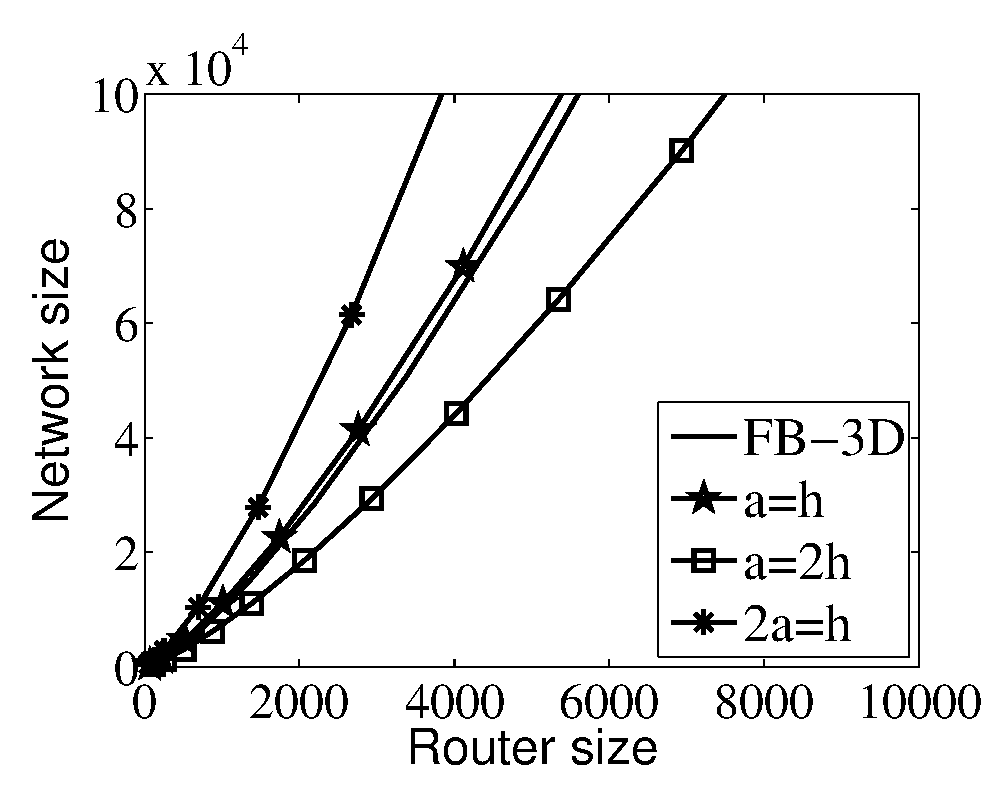
\includegraphics[width=.4\textwidth]{BB_1_v14.eps}
      \label{fig:bbw_3dfb_b}
    }
    \\
    \subfloat[网络直径$D=5$]{
      \includegraphics[width=.4\textwidth]{bbw_5dfb_a}
      %% 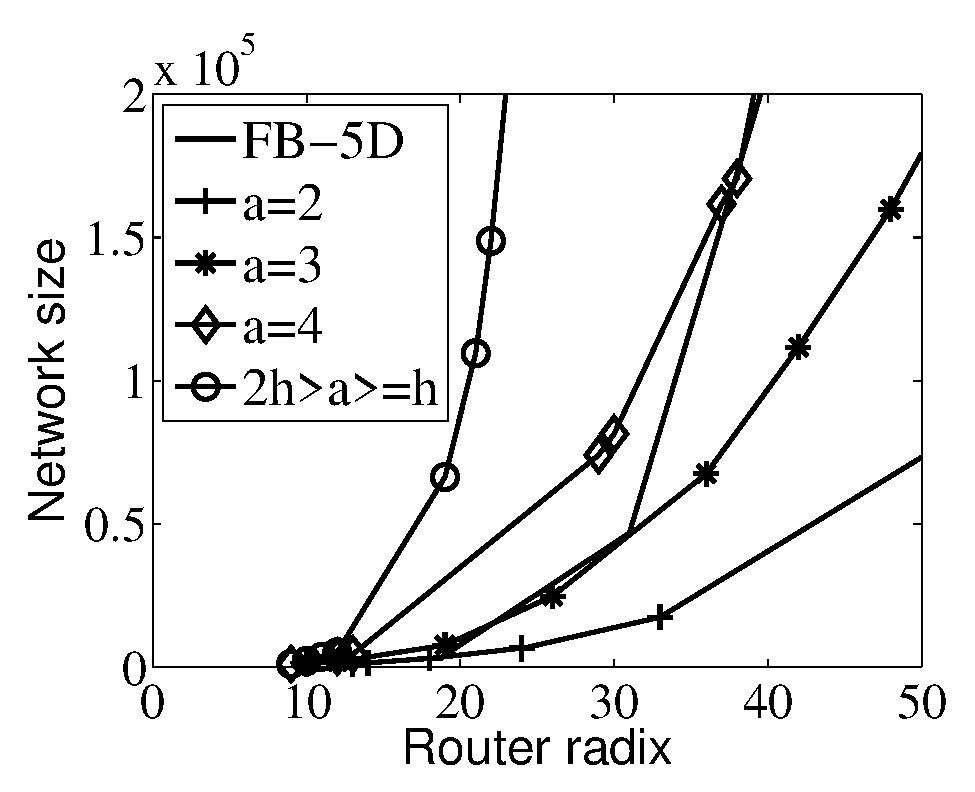
\includegraphics[width=.4\textwidth]{BB_1_v15.eps}
      \label{fig:bbw_5dfb_a}
    }
    \subfloat[网络直径$D=5$]{
      \includegraphics[width=.4\textwidth]{bbw_5dfb_b}
      %% 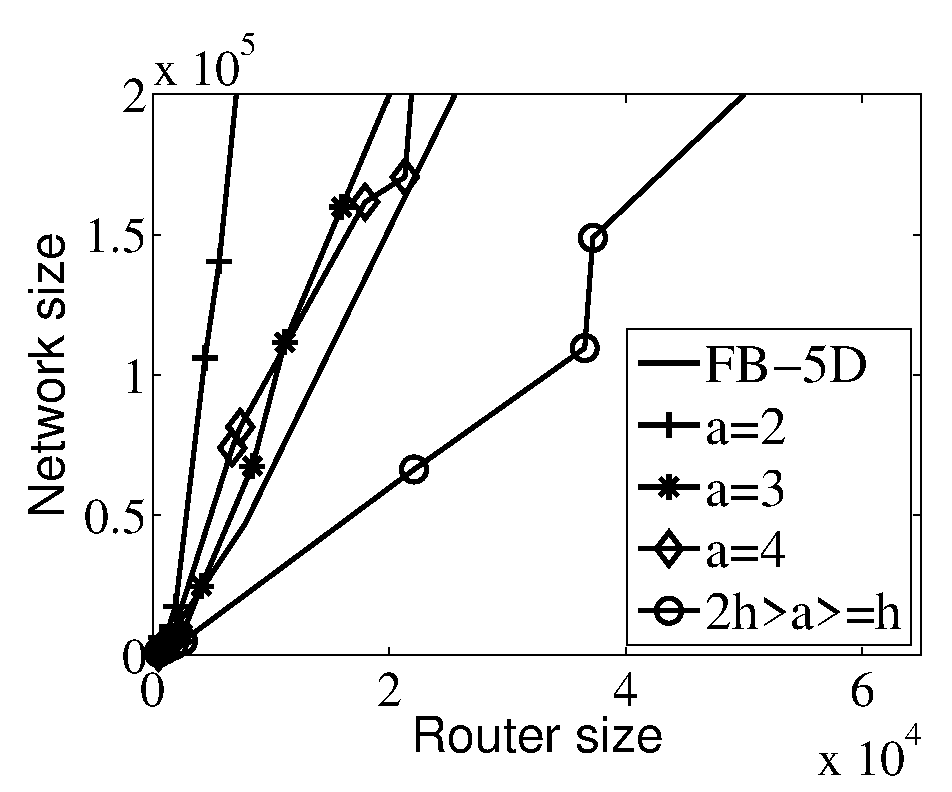
\includegraphics[width=.4\textwidth]{BB_1_v16.eps}
      \label{fig:bbw_5dfb_b}
    }
    \caption{Galaxyfly在$\beta \approx 0.5$时的网络规模与路由器总数}
    \label{chap03figure6}
  \end{minipage}
\end{figure}

图\ref{fig:bbw_sf_a}、图\ref{fig:bbw_3dfb_a}和图\ref{fig:bbw_5dfb_a}
描述了随着端口数$r$增加,网络规模$N$的变化趋势。
相应地,图\ref{fig:bbw_sf_b}、图\ref{fig:bbw_3dfb_b}和图\ref{fig:bbw_5dfb_b}
描述了随着网络规模$N$的增加,路由器数量$N_r$的增长趋势。
图\ref{fig:bbw_sf_a}与图\ref{fig:bbw_sf_b}展示了直径为2的网络SF与GF$(n,q,a=1,p,h)$。
对于GF,我们选择了三种不同的$n$和$q$的比例。
由图可知,使用同样的路由器端口数$r$,SF可以构造最大规模的直径为2的网络,
但是,在同一规模下,GF$(n=q,q,a=1,p,h)$和GF$(n=2q,q,a=1,p,h)$
使用的路由器数量比SF更少。
图\ref{fig:bbw_3dfb_a}与图\ref{fig:bbw_3dfb_b}展示了直径为3的网络3D FB与GF$(n,q=q,a,p,h)$。
这里的GF$(n,q=1,a,p,h)$本质上就是DF结构。
我们选择了三种不同的$a$和$h$的比例。
当$a=2h$时(此时$n=a^{2}/2+1$),GF$(n,q=1,a,p,h)$网络均衡且规模最大,
它比3D FB结构的扩展性好。
但是,在限定路由器端口数为48时,其最大规模仍然不能达到100K。
图\ref{fig:bbw_5dfb_a}与图\ref{fig:bbw_5dfb_b}展示了直径为5的网络5D FB与GF$(n=q,q,a,p,h)$。
对于GF的参数$a$,我们选择了四种不同的值。
由图可知,5D FB、GF$(n=q,q,a=4,p,h)$与GF$(n=q,q,h\leq{}a<2h,p,h)$在使用48端口的路由器时
可以构造100K规模的网络。
其中,GF$(n=q,q,h\leq{}a<2h,p,h)$使用路由器最多,
但是,它需要的路由器的端口数是最小。
在网络规模为200K 时,GF$(n=q,q,h\leq{}a<2h,p,h)$需要的路由器端口数仅为5D FB的一半。

我们还分析了不同$\beta$下,路由器数量和网络规模的关系。
表\ref{chap3table5}列出了一些GF和DF实例的$\beta$、路由器数量$N_r$与网络规模$N$,
这些GF与DF实例采用相同的配置$a=2h=2p$。
从表中可以看出,$\beta$的值越高,则需要更多的路由搭建同一规模的网络。
GF的规模可以达到接近$a^2/4$倍DF的规模,而其其二分带宽只是稍微低于DF。
因此,在满足给定二分带宽需求的前提下,GF可以使用同样的路由器构造更大规模的网络。

%% FIXME 表里的r是多少?为什么不把N也列出来?
%% (n-1+2ell)/a=h
%% r=a-1+h+p
\begin{table}[t]
\caption{同样参数配置$a$、$h$和$p$的Galaxyfly和Dragonfly的二分带宽}
\centering
\begin{tabular}{cccccc}
  \toprule
  Topology & GF$(n,q,a,p,h)$ & r & $N_r$ & \tabincell{c}{二分带宽}	& $\beta$\\
  \midrule
  \multirow{5}*{DF}
  &$GF(9,1,4,2,2)$	& 7 & 36	&20	&0.56 \\
  &$GF(19,1,6,3,3)$	& 11 &114	&94	&0.55 \\
  &$GF(33,1,8,4,4)$	& 15 &264	&275	&0.52 \\
  &$GF(55,1,10,5,5)$	& 19 &550	&701	&0.51 \\
  &$GF(73,1,12,6,6)$	& 23 &876	&1332	&0.51 \\
  \midrule
  \multirow{5}*{GF}
  &$GF(5,7,4,2,2)$	& 7 &140	&44	&0.31	\\
  &$GF(9,19,6,3,3)$	& 11 &1026	&560	&0.36 \\
  &$GF(17,31,8,4,4)$	& 15 &4216	&2350	&0.28 \\
  &$GF(30,53,10,5,5)$	& 20 &15900	&14026	&0.35 \\ %这个根本不是可行配置
  &$GF(37,73,12,6,6)$	& 23 &32412	&36676	&0.38 \\
  \bottomrule
\end{tabular}
 \label{chap3table5}
\end{table}

二分带宽是一个理论指标,是网络平均二分之间的带宽上限,
给定不同通信模式和不同路由算法,有效的二分带宽小于理论的二分带宽\upcite{multistage}。

\subsection{最短路径}

最短路径数量是一个负载均衡的网络重要的指标。表\ref{Tablesp}
列出了不同配置下的GF与SF的最短路径数量。$SP$是指最短路径数量大于1
的节点对数量与网络中所有节点对总数$N_r(N_r-1)/2$的比值。
集群内$SP$是指集群内最短路径数大于1的节点对数量与网络中所有节点对总量的比值,
对应地,集群间$SP$指集群间最短路径数大于1的节点对数量与网络中所有节点对总数的比值。
对于SF,尽管在限定网络直径为2的情况下可以构造最大规模的网络,
但是其最短路径数量却远远小于表中列出的GF配置。
GF$(n>1,q>1,a=1,p,h)$也是一个直径为2的拓扑结构,
与SF相比,它的SP更高,但用于连接其他路由器的端口数$h+a-1$也更大,
这使得GF$(n>1,q>1,a=1,p,h)$拥有多于SF的链路数量。
GF$(n>1,q=1,a>1,p,h)$是DF结构,它的$SP$值略大于GF$(n<1,q>1,a=1,p,h)$的SP,
且使用了更少的端口数,但集群内的最短路径数少。
GF$(n>1,q>1,a>1,p,h)$的SP最高而且使用的路由器端口数最少,
然而它的网络直径是5,是表中列出的网络中直径最大的一个。绝大多数集群内
$SP$是低于集群间$SP$的,因此,为了提高网络的负载均衡,
应该尽量充分利用集群间的最短路径数量。

\begin{table}[t]
\caption{Galaxyfly与Slim Fly的最短路径数量}
\centering
\begin{tabular}{cccccc}
  \toprule
  拓扑结构 & $h+a-1$ & $N_r$ & $SP$ & 集群内$SP$ & 集群间$SP$\\
  \midrule
  \multirow{2}*{$SF$}
  &25		&578	 &0.01 &0.01 & 0 \\ %\cline{2-6}
  &35		&1058	 &0.05 &0.01 & 0.04\\
  \midrule
  \multirow{2}*{$GF(n\!\!>\!\!1,q\!\!>\!\!1,a\!\!=\!\!1,p,h)$}
  &31		&496	&0.14 &0.03 &0.11\\
  &47		&992	&0.13 &0.01 &0.12\\
  \midrule
  \multirow{2}*{$GF(n\!\!>\!\!1,q\!\!=\!\!1,a\!\!>\!\!1,p,h)$}
  &14		&510	&0.17 &0 &0.17\\
  &17		&876	&0.15 &0 &0.15\\
  \midrule
  \multirow{2}*{$GF(n\!\!>\!\!1,q\!\!>\!\!1,a\!\!>\!\!1,p,h)$}
  &8		&510	&0.43 &0.03 &0.41\\
  &8		&966	&0.51 &0.06 &0.44\\
  \bottomrule
\end{tabular}
\label{Tablesp}
\end{table}

\subsection{容错性}

我们通过模拟随机链路的出错来分析拓扑结构的容错性。
采用的具体方法是,逐渐提升网络链路随机出错的概率直至网络不连通,
观察网络的平均路径长度与网络直径如何随链路出错率变化而变化。
图\ref{fig:Figure8a}与图\ref{fig:Figure8b}
分别展示了不同配置下的GF和其他拓扑结构的平均最短路径和网络直径
随着链路出错率增加而变化的情况。
图\ref{nr1}和图\ref{nr2}展示了GF$(n>1,q>1,a=1,p,h)$和SF在路由器
规模在0.2K-2K范围内容错性的变化情况。
图\ref{nr3}和图\ref{nr4}展示了GF$(n>1,q>1,a>1,p,h)$和DF在路由器
规模在0.2K-2K范围内容错性的变化情况。
对于GF、DF和SF,容错性随着路由器规模的增加而提升。
在路由器规模为2K的情况下,GF$(n>1,q>1,a=1,p,h)$可以容忍$90\%$的链路出错率,
而SF的链路错误容忍度为$86\%$。
GF$(n>1,q>1,a>1,p,h)$和DF分别只能容忍$60\%$和$65\%$的链路出错率。
GF$(n>1,q>1,a=1,p,h)$和SF的容错性能比GF$(n>1,q>1,a>1,p,h)$和DF
在同一规模下容错性好是因为更短的网络直径和更多的链路。

\begin{figure}
  \centering
  \begin{minipage}[t]{\textwidth}
    \centering
    \subfloat[平均路径长度]{
      \includegraphics[width=.4\textwidth]{resiliency_a}
      \label{nr1}
    }
    \subfloat[网络直径]{
      \includegraphics[width=.4\textwidth]{resiliency_b}
      \label{nr2}
    }
    \caption{$GF(n\!\!>\!\!1,q\!\!>\!\!1,a\!\!=\!\!1,p,h)$与SF的容错性}
  \label{fig:Figure8a}
  \end{minipage}
\end{figure}
\begin{figure}
  \centering
  \begin{minipage}[t]{\textwidth}
    \centering
    \subfloat[平均路径长度]{
      \includegraphics[width=.4\textwidth]{resiliency_c}
      \label{nr3}
    }
    \subfloat[网络直径]{
      \includegraphics[width=.4\textwidth]{resiliency_d}
      \label{nr4}
    }
    \caption{$GF(n\!\!>\!\!1,q\!\!>\!\!1,a\!\!>\!\!1,p,h)$与DF的容错性}
    \label{fig:Figure8b}
  \end{minipage}
\end{figure}


\section{路由算法}

本节将给出Galaxyfly结构的最短路径路由算法与非最短自适应路由算法,
并介绍与路由算法配套的死锁避免机制。在本节路由算法的讨论中,
假设报文从源节点直接传输给直接相连的源路由节点$R_s$并由此路由至与目的节
点直接相连的目的路由节点$R_d$。

\subsection{最短路径路由算法}

%% 由于Galaxyfly是将Galaxy图中的节点代之以$a$个路由器全互连组成的超级节点得到
%% 的层次化互连网络,因此Galaxyfly网络的最短路由算法中最段路径的计算
%% 可以分层进行。即,先寻找超级节点$G_s$与$G_d$之间的最短路径,
%% 在此基础上计算路由节点$R_s$与$R_d$之间的最短路径。

%% 上述思路不正确
%% 路由节点间的最短路径并不一定通过所在超级节点间的最短路径

\begin{algorithm}[t]
  \caption{Galaxyfly网络最短路径算法}
  \label{alg:min}
  \algsetup{indent=1em}
  \begin{algorithmic}[1]
    \REQUIRE 源路由节点$R_s$
    \ENSURE $R_s$到所有其他路由节点$R_d$的最短路径集合$P_{s,d}$,
    %% $\P_{s,d} = \{P_{s,d}^0, P_{s,d}^1, \cdots, P_{s,d}^{K_{s,d}-1}\}$,\\
    其中$d \in [0, N_r)$且$d \neq s$
    \STATE $P_{s,s} \gets \lbrace [R_s] \rbrace$ \label{l:res.init.self}
    \FOR {$d \in [0, N_r) \land d \neq s$} \label{l:res.init.begin}
    \STATE $P_{s,d} \gets \emptyset$
    \ENDFOR \label{l:res.init.end}
    \STATE $V \gets \lbrace R_s \rbrace$ \label{l:v}
    \STATE $Q_c \gets \lbrace R_s \rbrace$ \label{l:qc}
    \STATE $Q_n \gets \emptyset$ \label{l:qn}
    \WHILE {$Q_c \neq \emptyset$} \label{l:bfs.begin}
    \FOR {$R \in Q_c$} \label{l:expand.begin}
    \STATE $Q_n \gets Q_n \bigcup (neighbors(R) - V)$
    \ENDFOR \label{l:expand.end}
    \FOR {$R_d \in Q_n$} \label{l:rd}
    \FOR {$R_x \in neighbors(R_d) \bigcap V$} \label{l:rx}
    \STATE $P_{s,d} = \lbrace\ append(p, R_d)\ |\ \forall p \in P_{s,x}\ \rbrace$ \label{l:psd}
    \ENDFOR
    \ENDFOR
    \STATE $Q_c \gets Q_n$ \label{l:qc.update}
    \STATE $Q_n \gets \emptyset$ \label{l:qn.update}
    \ENDWHILE \label{l:bfs.end}
  \end{algorithmic}
\end{algorithm}

Galaxyfly网络中节点间最短路径可能不唯一,
在报文从源路由节点$R_s$向目的路由节点$R_d$的传输过程中,
应尽量均衡地利用多个最短路径以平衡网络负载。
因此,最短路径路由算法应记录任意节点对$R_s$、$R_d$之间的所有最短路径。
算法\ref{alg:min}给出了计算Galaxyfly网络中给定源路由节点$R_s$到
其他所有路由节点的最短路径集合的算法。
Galaxyfly是一个无向、无环、连通图,
算法\ref{alg:min}是一个基于宽度优先搜索(BFS)的遍历算法,
在搜索过程中完成$R_s$到任意节点$R_d$最短路径集合$P_{s,d}$的计算。
首先,$R_s$到自身的最短路径初始化为$\{[R_s]\}$(第\ref{l:res.init.self}行),
$R_s$到所有其他路由节点$R_d$的最短路径集合初始化为空集
(第\ref{l:res.init.begin}--\ref{l:res.init.end}行)。
之后,建立三个辅助数据结构$V$,$Q_c$,$Q_n$,
其中$V$表示已经访问过的节点集合(第\ref{l:v}行),
$Q_c$与$Q_n$分别表示BFS过程中当前正在扩展的节点集合与
下一次将要扩展的结点集合(第\ref{l:qc}--\ref{l:qn}行)。
算法的主循环(第\ref{l:bfs.begin}--\ref{l:bfs.end}行)执行BFS过程。
在BFS过程的每一次迭代中,
首先将$Q_c$中每个路由节点$R$的未访问过的邻居节点加入$Q_n$
(第\ref{l:expand.begin}--\ref{l:expand.end}行)。
然后,对$Q_n$中每一个路由节点$R_d$(第\ref{l:rd}行),
开始计算$R_s$到$R_d$的最短路径集合$P_{s,d}$,
具体方法如下:对于$R_d$的邻居节点$R_x$,如果$R_x \in V$,即$R_x$已经访问过(第\ref{l:rx}行),
那么将$R_d$添加到从$R_s$到$R_x$的任意最短路径$p$尾部即可得到一条
从$R_s$到$R_d$的最短路径(第\ref{l:psd}行)。
最后,更新扩展队列集合$Q_c$与$Q_n$(第\ref{l:qc.update}--\ref{l:qn.update}行)。

%% \begin{algorithm}[t]
%%   \caption{Galaxyfly网络最短路径算法}
%%   \label{alg:min}
%%   \algsetup{indent=1em}
%%   \begin{algorithmic}[1]
%%     \REQUIRE 源路由节点$R_s$,目标路由节点$R_d$
%%     \ENSURE $R_s$到$R_d$的最短路径集合$P_{min} = \{P_0, P_1, \cdots, P_{K-1}\}$,其中\\
%%     $P_k=[R_k^0, R_k^1, \cdots, R_k^{n-1}]$,$k \in [0, K)$为$R_s$到$R_d$的一条长度为$n$的最短路径
%%     \STATE $P_{min} \gets \emptyset$
%%     \STATE $G_s \gets supernode(R_s)$
%%     \STATE $G_d \gets supernode(R_d)$
%%     \IF {$G_s = G_d$}
%%     \STATE $P_{min} \gets \{[R_s, R_d]\}$
%%     \ELSIF {connected($G_s$, $G_d$)}
%%     \STATE $S \gets \{\ R_x\ |\ \forall (R_x, R_y) \in edges(G_s, G_d)\ \}$
%%     \STATE $D \gets \{\ R_y\ |\ \forall (R_x, R_y) \in edges(G_s, G_d)\ \}$
%%     \IF {$R_s \in S \land R_d \in D$}
%%     \STATE $P_{min} \gets \{\ [R_s, R_d]\ \}$
%%     \ELSIF {$R_s \in S \land R_d \notin D$}
%%     \STATE $P_{min} \gets \{\ [R_s, R_y, R_d]\ |\ \forall R_y \in D \land (R_s, R_y) \in edges(G_s, G_d)\ \}$
%%     \ELSIF {$R_s \notin S \land R_d \in D$}
%%     \STATE $P_{min} \gets \{\ [R_s, R_x, R_d]\ |\ \forall R_x \in S \land (R_x, R_d) \in edges(G_s, G_d)\ \}$
%%     \ELSIF {$R_s \notin S \land R_d \notin D$}
%%     \STATE $P_{min} \gets \{\ [R_s, R_x, R_y, R_d]\ |\ \forall (R_x, R_y) \in edges(G_s, G_d)\ \}$
%%     \ENDIF
%%     \ELSE
%%     \STATE $GG \gets \{\ G_m\ |\ connected(G_s, G_m) \land connected(G_m, G_d)\ \}$
%%     \FOR {$G_m \in GG$}
%%     \STATE $t_m \gets 5$
%%     \STATE $S \gets \{\ R_x\ |\ \forall (R_x, R_y) \in edges(G_s, G_m)\ \}$
%%     \STATE $M_S \gets \{\ R_y\ |\ \forall (R_x, R_y) \in edges(G_s, G_m)\ \}$
%%     \STATE $M_D \gets \{\ R_x\ |\ \forall (R_x, R_y) \in edges(G_m, G_d)\ \}$
%%     \STATE $D \gets \{\ R_y\ |\ \forall (R_x, R_y) \in edges(G_m, G_d)\ \}$
%%     \IF {$R_s \in S$}
%%     \STATE $t_m \gets t_m - 1$
%%     \ENDIF
%%     \ENDFOR
%%     \ENDIF
%%   \end{algorithmic}
%% \end{algorithm}

为得到Galaxyfly网络中所有节点对之间的最短路径,
只需对所有路由节点运行一次算法\ref{alg:min}即可。
完成所有路由节点对的最短路径计算后,
可以通过配置路由表等方式实现最短路由算法MIN,
在路径选择方面可以使用简单的令牌方式均衡使用不同的最短路径。

\subsection{非最短路径自适应路由算法}

我们为Galaxyfly设计了三种非最短自适应路由算法,分别是
非最短自适应随机链路路由算法(NAR),
非最短自适应本地链路路由算法(NAL),以及
非最短自适应全局链路路由算法(NAG),
他们都是基于Galaxyfly结构特性、非最短路径路由算法以及全局
自适应负载均衡路由算法设计的\upcite{Singh}\upcite{slimfly}\upcite{dragonfly}。
为了控制两个终端的之间的跳步数和减少虚拟通道(VC)的数量,非最短
自适应路径会限制随机选择路径的长度。
NAR使用的策略是,只有当两个终端处于同一个集群的两个不同的超级节点时,
才会执行非最短路由,选择的非最短路径通过两个超级节点的公共邻超级节点,
该策略的目的是限制非最短路由的路径长度,使得非最短路径长度最多为5跳。
NAL的策略是是允许在源超级节点内多绕行1跳,其非最短路径的长度限制为6跳。
NAG的策率则是允许绕行到别的超级节点,其非最短路径的长度限制为7跳,
(3跳超级节点间链路与4跳超级节点内的链路)。

非最短路径自适应路由主要用于最短路径过载的情况下。
网络负载状态的判定在路由器本地完成,
主要依据为当前路由器的缓冲区状态。
具体来说,是根据缓冲区队列的占有率来选择使用最短路径路由或是非最短路径自适应路由。
令$Q_{min}$与$Q_{nonmin}$分别表示最短路径端口与非最短路径端口的缓冲区队列的占有率,
$Th_{min}$和$Th_{nonmin}$分别表示选择走最短路径和非最短路径的阈值。
若$Q_{min}>Th_{min}$且$Q_{nonmin}<Th_{nonmin}$,那么报文将通过非最短路径传输。
$Th_{nonmin}$和$Th_{min}$是经验参数,可以通过模拟进行调优。
%% 在我们的实验中,这两个阈值分别被设置为
%% $Th_{nonmin}=0.5Q_{min}$ 和 $Th_{min}=0.8\times$ $缓冲区容量$。

\subsection{死锁避免机制}

Galaxyfly的死锁避免机制与Dragonfly\upcite{dragonfly}和
Slim Fly\upcite{slimfly}的死锁避免机制类似。
基于距离的死锁避免机制每一跳都切换一条VC,
因此,需要的VC数量与最长路径跳步数相同。
在Galaxyfly结构中,我们使用递增的方法分配VC。
即,报文开始注入时使用编号为0的VC,每经过一跳使用的
VC编号加一\upcite{Prevention}\upcite{Rlmolm}。
报文在最后一条VC的时候不会被堵塞是因为报文要被吸收。
因此,报文要么前进走更高编号的VC,要么就是要被终端吸收。
由于Galaxyfly划分了超级节点,我们能复用本地端口的VC和全局端口的VC,
这样可以减少VC的数量。

图\ref{fig:Figure9}说明了不同网络直径的Galaxyfly网络中
最短路径路由是如何使用VC的避免死锁的。
例如,在图\ref{fig:Figure93}所示的最短路径路由中,
报文最多经过3条本地链路和2条全局链路。
因此,在MIN中要求至少3条本地链路VC和2条全局链路VC来避免出现环,
然而,由于由于我们复用了本地端口与全局端口的VC,
我们一共只需要3条VC既可以避免死锁。
类似地,NAR、NAL以及NAG算法分别需要3、4、4条本地链路VC和2、2、3条全局链路VC,
考虑到VC复用,它们分别需要3、4、4条VC来避免死锁。

除上述依赖VC的死锁避免机制以外,Galaxyfly也可以使用逃逸网络或者转弯模型方法来避免死锁
\upcite{Rlmolm}\upcite{OFAR-CM}\upcite{On-the-Fly}。

\begin{figure}[t]
  \centering
   \begin{minipage}[t]{\textwidth}
   \centering
  \subfloat[网络直径$D=2$]{
  \includegraphics[width=.25\textwidth]{Visiomind1.eps}
  \label{fig:Figure91}
  }
  \subfloat[网络直径$D=3$]{
  \includegraphics[width=.5\textwidth]{Visiomind2.eps}
  \label{fig:Figure92}
  }
  \\
  \subfloat[网络直径$D=5$]{
  \includegraphics[width=.75\textwidth]{Visiomind3.eps}
  \label{fig:Figure93}
  }
  \caption{Galaxyfly最短路径路由算法中的VC使用}
  \label{fig:Figure9}
  \end{minipage}
\end{figure}

\section{性能分析}

在这一章节中,我们使用一个时钟精确的网络模拟器Booksim\upcite{Booksim}模拟Galaxyfly
和其他拓扑结构的运行来分析比较不同拓扑结构的性能。
实验采用伯努力分布报文注入模型。
首先,我们在几种典型的通信模式下评测了不同配置下的Galaxyfly网络,
分析了在不同的报文长度及不同路由算法下的网络性能。
第二,我们比较了Galaxyfly和其他高阶拓扑结构在不同的通信模式下的性能,
包括一种新的混合通信模式。
第三,我们在物理布局对网络延迟产生影响的情况下评测了不同拓扑结构的性能。

\subsection{实验设置}

\subsubsection{路由器}

我们使用传统的具备完整的路由器流水线的输入队列(Input Queue,IQ)路由器模型。
路由器基于Virtual Cut-through(VCT)交换机制。
我们假设信用处理过程需要2个时钟周期,路由计算模块需要2个时钟周期,
交换分配模块、虚通道(VC)分配模块和crossbar处理模块都需要1个时钟周期,
crossbar的输入和输出的加速比都是1,内部传输数据链路速率是链路传输速率的两倍。
路由器每个输入端口的缓冲区容量是256个切片。
缓冲区的管理机制采用每个VC拥有5个切片的私有存储空间,
其他的缓冲区由所有VC共享。

\subsubsection{网络类型}
我们提供了两种链路传输延迟配置。
一种是每一条链路的传输延迟都是1个时钟周期。
在这种配置下,我们可以减少不同拓扑结构在构造同等规模的网络时
使用不同端口数的路由器而造成的影响并观察网络状态。
在文献\upcite{slimfly}与文献\upcite{dragonfly}中,
链路传输延迟即采用这种配置。
第二种配置是根据物理布局中的位置设置延迟,
其目的是为了模拟实际系统物理布局对延迟造成的影响。
机柜间链路包括路由器流水线的延迟一共100个周期,
而机柜内链路则是50个周期。

表\ref{chap3table6}列出了实验中选用的所有拓扑结构及其参数配置。
其中,Fat tree(FT)是高性能计算系统和数据中心系统最常用的拓扑结构之一,
Flattened Butterfly(FB)和Dragonfly(DF)是高阶互连网络的典型拓扑结构,
Slim Fly(SF)则是最新提出的低直径高性能互连拓扑结构。
表\ref{chap3table6}中所有的拓扑结构的最小二分切割都包含至少$N/4$条双向链路,
在均衡随机通信负载下的二分带宽都满足$\beta>0.5$,
构建的网络的规模约为$N\approx 3K$,
不同的拓扑结构在规模上的差别不超过10\%。

\begin{table}[t]
\caption{拓扑结构及其配置}
\centering
\begin{tabular}{cccccc}
  \toprule
  Topology	& $r$ &$p$ & Diameter & $N_r$ 	& $\beta$ \\
  \midrule
  GF$(11,29,1,10,24)$ &34 &10 &2	&319 		&0.60	\\
  GF$(15,29,1,7,28)$ &35 &7 &2	&435 		&1.12 \\
  GF$(56,1,11,5,5)$ &20 &5 &3	&616 		&0.51 \\
  GF$(81,1,10,4,8)$ &21 &4 &3	&810 	&1.01 \\
  GF$(11,29,2,5,12)$ &18 &5 &4	&638 		&0.59 \\
  GF$(15,37,2,3,16)$ &20 &3 &4	&1110 		&1.13 \\
  GF$(11,37,4,2,7)$ &12 &2 &5	&1628 		&0.62 \\
  GF$(15,29,4,2,7)$ &12 &2 &5	&1740 		&0.68 \\
  FT &30 &15 &4	&675		&1	\\
  FB &27 &6	  &3 &512		&1.33 \\
  SF &29 &10 &2	&338		&0.65 \\
  DF &20 &5	&3 &616		&0.50 \\
  \bottomrule
\end{tabular}
  \label{chap3table6}
\end{table}

\subsubsection{路由算法}
实验中对不同拓扑结构,采用了不同的路由算法测试性能。
其中,FT拓扑采用了自适应最近公共祖先(ANCA)路由算法,
DF\upcite{dragonfly}、FB\upcite{Flattenedbutterfly}、 SF\upcite{slimfly}
以及GF采用了最短路径路由算法(MIN)和基于本地缓冲区队列大小的非最短自适应路由算法。

\subsubsection{通信模式}
我们采用典型的高性能工作负载通信模式去评测不同的拓扑结构,
包括均衡随机通信模式,最差通信模式,以及混合通信模式。

在均衡随机通信模式下,报文的源节点和目的节点都是随机选择。
这种通信模式常见于图计算、稀疏线性线代数求解以及自适应mesh分布方法等高性能应用。

最差通信模式用于模拟报文的源节点和目的节点相距最远且一些链路高频率使用导致拥塞的情况。
在FT中,传输报文必须通过最高层的路由节点。
在DF中,报文的源节点和目的节点在两个不同超级节点内
而且两个超级节点内的节点互相通信造成超级节点间的链路拥塞。
在SF中,通信只发生在两个终端在同一个子图内的不同子组之间\upcite{slimfly}。
FB的最差通信模式与$k-ary$ $n-cube$的飓风通信模式类似。
在GF中,通信只发生在不同集群之间。

在高性能计算工作负载中,不同节点通信类型的异质性是不可忽略的
\upcite{Mubarak2017Quantifying} \upcite{Gliksberg2018Node}。
因此,我们设计了一种混合通信模式用于评测拓扑结构在混合工作负载下的性能。
该混合通信负载包括$90\%$的均衡随机通信模式用于模拟计算节点之间通信,
$10\%$的热点通信模式用于模拟计算节点和固定范围的I/O节点通信。

\subsection{Galaxyfly性能分析}
本节分析参数配置、报文长度、路由算法对Galaxyfly网络性能的影响。

\subsubsection{参数配置}

\begin{figure}[t]
  \centering
  \begin{minipage}[t]{\textwidth}
    \centering
    \subfloat[网络直径$D=2$]{
      \includegraphics[width=.4\textwidth]{gf_ur_a}
      %% \includegraphics[width=.4\textwidth]{gf_un1.eps}
      \label{gf_un1}
    }
    \subfloat[网络直径$D=3$]{
      \includegraphics[width=.4\textwidth]{gf_ur_b}
      %% \includegraphics[width=.4\textwidth]{gf_un2.eps}
      \label{gf_un2}
    }
    \\
    \subfloat[网络直径$D=4$]{
      \includegraphics[width=.4\textwidth]{gf_ur_c}
      %% \includegraphics[width=.4\textwidth]{gf_un3.eps}
      \label{gf_un3}
    }
    \subfloat[网络直径$D=5$]{
      \includegraphics[width=.4\textwidth]{gf_ur_d}
      %% \includegraphics[width=.4\textwidth]{gf_un4.eps}
      \label{gf_un4}
    }
    \caption{不同参数配置下Galaxyfly网络性能(均衡随机通信模式)}
    \label{chap3figure10a}
  \end{minipage}
\end{figure}
\begin{figure}
  \centering
  \begin{minipage}[t]{\textwidth}
    \centering
    \subfloat[网络直径$D=2$]{
      \includegraphics[width=.4\textwidth]{gf_w_a}
      %% \includegraphics[width=.4\textwidth]{gf_un5.eps}
      \label{gf_un5}
    }
    \subfloat[网络直径$D=3$]{
      \includegraphics[width=.4\textwidth]{gf_w_b}
      %% \includegraphics[width=.4\textwidth]{gf_un6.eps}
      \label{gf_un6}
    }
    \\
    \subfloat[网络直径$D=4$]{
      \includegraphics[width=.4\textwidth]{gf_w_c}
      %% \includegraphics[width=.4\textwidth]{gf_un7.eps}
      \label{gf_un7}
    }
    \subfloat[网络直径$D=5$]{
      \includegraphics[width=.4\textwidth]{gf_w_d}
      %% \includegraphics[width=.4\textwidth]{gf_un8.eps}
      \label{gf_un8}
    }
    \caption{不同参数配置下Galaxyfly网络性能(最差通信模式)}
    \label{chap3figure10b}
  \end{minipage}
\end{figure}

我们根据网络直径将表\ref{chap3table6}中列出的不同配置下的Galaxyfly网络划分成组,
比较组内Galaxyfly网络的性能。
图\ref{chap3figure10a}与\ref{chap3figure10b}分别展示了
在均衡随机通信模式与最差通信模式下的性能测试结果。
对照表\ref{chap3table6}可知,
%% GF$(15,29,1,7,28)$、GF$(81,1,10,4,8)$、GF$(15,37,2,3,16)$和GF$(15,29,4,2,7)$的二分带宽
%% 分别高于GF$(11,29,1,10,24)$、GF$(56,1,11,5,5)$、GF$(11,29,2,5,12)$和GF$(11,37,4,2,7)$,
%% 观察图\ref{chap3figure10a}与\ref{chap3figure10b}可知,
无论在均衡随机通信模式或者是最差通信模式下,
网络的二分带宽越高,其饱和吞吐率越高。
以图\ref{gf_un1}和图\ref{gf_un5}为例,
GF$(15,29,1,7,28)$的路由器数量与最小二分切割的链路数分别比
GF$(11,29,1,10,24)$高36.3\%与79.5\%,
在两种通信模式下,GF$(15,29,1,7,28)$的饱和吞吐率比GF$(11,29,1,10,24)$分别高21.5\%和55.6\%。
然而,网络直径更短以及二分带宽更高的配置不一定能获得高的饱和吞吐率。
虽然GF$(15,37,2,3,16)$ 的网络直径为4 且$\beta>1$,
在均衡随机通信模式下,GF$(15,37,2,3,16)$的饱和吞吐率为0.15,
仅能达到GF$(11,37,4,2,7)$饱和吞吐率的33\%,
原因在于前者的超级结点内部全互连本地网络二分带宽不足,
超级结点内部发生了阻塞。

\subsubsection{报文长度}

我们分析不同的报文长度如何影响Galaxyfly的网络性能。
图\ref{fig:packetsize}展示了不同通信模式下使用不同报文长度的性能测试结果。
由该图可知,在同样配置的Galaxyfly网络中,
报文长度越短,网络延迟越小,但是长报文的饱和吞吐率更高,
对于网络直径较短的Galaxyfly网络尤其如此。
\begin{figure}
  \centering
  \begin{minipage}[t]{\textwidth}
    \centering
    \subfloat[均衡随机通信模式]{
      \includegraphics[width=.4\textwidth]{packets_a}
      %% \includegraphics[width=.4\textwidth]{lap3.eps}
      \label{lap3}
    }
    \subfloat[最差通信模式]{
      \includegraphics[width=.4\textwidth]{packets_b}
      %% \includegraphics[width=.4\textwidth]{lap4.eps}
      \label{lap4}
    }
    \caption{不同报文长度下Galaxyfly的网络性能}
    \label{fig:packetsize}
  \end{minipage}
\end{figure}

\subsubsection{路由算法}

大规模的高性能计算系统,通信模式更加复杂多样。
我们引进了一种混合通信模式评测路由算法性能,
该混合通信负载包括$90\%$的均衡随机通信模式用于模拟计算节点之间通信,
$10\%$的热点通信模式用于模拟计算节点和固定范围的I/O节点通信。
图\ref{lbr2}展示了GF$(15,29,4,2,7)$在混合通信模式下四种不同路由算法的性能
(其他配置的Galaxyfly也呈现相似的结果)。
NAG算法相比其他路由算法表现出更优的性能。
为定量分析NAG的性能优势,我们分别测试了NAG算法与MIN算法在
不同配置Galaxyfly网络中的性能,结果如图\ref{lbr3}。
在GF$(15,29,1,7,28)$、GF$(15,29,4,2,7)$与GF$(81,1,10,4,8)$网络中,
NAG算法的饱和吞吐率比MIN算法分别高出25\%, 260\%, 与100\%。

\begin{figure}
  \centering
  \begin{minipage}[t]{\textwidth}
    \centering
    \subfloat[GF$(15,29,4,2,7)$]{
      \includegraphics[width=.4\textwidth]{routingalgos_a}
      %% \includegraphics[width=.4\textwidth]{lbr2.eps}
      \label{lbr2}
    }
    \subfloat[MIN与NAG的性能比较]{
      \includegraphics[width=.4\textwidth]{routingalgos_b}
      %% \includegraphics[width=.4\textwidth]{lbr3.eps}
      \label{lbr3}
    }
    \caption{不同路由算法下Galaxyfly的网络性能(混合通信模式)}
    \label{fig:routingalgorithms}
  \end{minipage}
\end{figure}

\subsection{不同拓扑结构的比较}


\subsubsection{与Fat tree的比较}
图\ref{fig:gfft}展示了不同配置的GF与FT的性能对比结果。
在两种通信模式下,GF$(15,29,1,7,28)$与GF$(81,1,10,4,8)$
都表现出比FT更低的网络延迟、更高的饱和吞吐率。
而且,GF$(15,29,1,7,28)$使用的路由器数量仅为FT的64\%。
GF$(15,29,1,7,28)$的性能优于FT有两个原因。
一是网络直径更短,GF$(15,29,1,7,28)$的网络直径为2。
而FT的网络直径更长,同时长路径路由增加了头阻塞的概率。
第二个原因则是较高的全局链路密度,
GF$(15,29,1,7,28)$中每一个路由器80\%的端口用于
互连其他超级节点的其他路由器。
GF$(15,29,4,2,7)$与GF$(81,1,10,4,8)$的路由器数量多于FT,
然而FT必须使用30端口路由器,而它们需要的路由器端口数分别为21与12,
仅为FT路由器端口数的70\%与40\%。
而且,GF$(81,1,10,4,8)$的网络直径为3,其网络延迟低于
Fat tree。

\begin{figure}
  \centering
  \begin{minipage}[t]{\textwidth}
    \centering
    \subfloat[均衡随机通信模式]{
      \includegraphics[width=.4\textwidth]{gfft_a}
      %% \includegraphics[width=.4\textwidth]{df_un1.eps}
      \label{df_un1}
    }
    \subfloat[最差通信模式]{
      \includegraphics[width=.4\textwidth]{gfft_b}
      %% \includegraphics[width=.4\textwidth]{df_un4.eps}
      \label{df_un4}
    }
    \caption{Galaxyfly与FT性能比较}
    \label{fig:gfft}
  \end{minipage}
\end{figure}

\subsubsection{与Flattened Butterfly的比较}
我们也比较了Galaxyfly和Flattened Butterfly的性能差别。
FB是一个高阶的$k-ary$ $n-cube$拓扑结构。
它在每一维上都是一个全互连的网络。
相比FT,FB的路由器数量和链路数更少。
图\ref{fig:gffb}展示了GF和3D FB的性能比较结果。
在均衡随机通信负载下,FB的性能跟GF$(81,1,10,4,8)$的相近,
其主要原因是因为两个网络有相同的网络直径。
虽然FB提供了多于GF$(81,1,10,4,8)$36\%的全局链路
(FB第一维的结构和GF$(81,1,10,4,8)$的超级节点被认为是本地组),
但是FB的全局链路集中在每一维上,而不是分布在整个全局网络上。
另外,在最差通信模式下,FB的饱和吞吐率
与GF$(15,29,4,2,7)$和GF$(81,1,10,4,8)$分别相差62.5\%和70\%。

\begin{figure}
  \centering
  \begin{minipage}[t]{\textwidth}
    \centering
    \subfloat[均衡随机通信模式]{
      \includegraphics[width=.4\textwidth]{gffb_a}
      %% \includegraphics[width=.4\textwidth]{df_un2.eps}
      \label{df_un2}
    }
    \subfloat[最差通信模式]{
      \includegraphics[width=.4\textwidth]{gffb_b}
      %% \includegraphics[width=.4\textwidth]{df_un5.eps}
      \label{df_un5}
    }
    \caption{Galaxyfly与FB性能比较}
    \label{fig:gffb}
  \end{minipage}
\end{figure}

\subsubsection{与Slim Fly和Dragonfly的比较}
图\ref{fig:gfsfdf}展示了不同配置的Galaxyfly与Slim Fly、Dragonfly的性能比较结果。

Slim Fly是最新提出的低直径高阶拓扑结构。
与Galaxyfly相同,Slim Fly也利用了代数图论有限域的方法。
Slim Fly保证网络直径为2,但是,它的低直径属性是基于路由器之间相连的端口数$k'$和路由器
规模$N_r$的最优关系,$k'\geq\Omega(\sqrt N_r)$。
该前提条件严格限制了Slim Fly的扩展性。
相对地,Galayxyfly支持使用固定端口数路由器构造任意规模系统。
GF$(n>1,q>1,a=1,p,h)$,即Galaxy图,也是一个直径为2的拓扑结构,
但在同样网络规模和相近的二分带宽要求下,它比SF需要更高的端口数。
比如,在表\ref{chap3table6}中,GF$(11,29,1,10,8)$
和Slim Fly具有相近的$\beta$,但是GF$(11,29,1,10,8)$的每一个路由器要求
更多的端口数。
GF$(15,29,1,7,28)$是另外一个直径为2的Galaxyfly配置,
具有更高的$\beta$值,也需要更高的路由器端口数。
因此,在Slim Fly和Galaxyfly的多种配置间中的选择,实际上
是性能和路由器端口数的权衡。
在均衡随机通信模式和最差通信模式下,
GF$(15,29,1,7,28)$的饱和吞吐率分别比SF高42\%和140\%。
其主要原因在于它比SF多使用了28\%的路由器和89\%的全局链路。
类似地,GF$(11,29,1,10,24)$在两种通信模式下的饱和吞吐率也分别比SF高8\%和60\%。
GF$(81,1,10,4,8)$是直径为3的网络,其零负载延迟略高于Slim Fly。
但是,在上述两种通信模式下,饱和吞吐率则分别高于SF近33\%和100\%。
而且,GF$(81,1,10,4,8)$的路由器端口数是21,仅为SF的75\%。

图\ref{fig:gfsfdf}中的DF结构本质上是GF$(56,1,11,5,5)$。
与DF相比,Galaxyfly不仅参数配置更加灵活而且能调整参数获得更好的网络性能。
GF$(81,1,10,4,8)$仅比DF多使用5\%的路由器端口,但是,
其性能在任一通信模式下都能优于DF一倍。
尽管GF$(15,29,4,2,7)$的零负载延迟高于DF,
但在均衡随机通信模式下,GF$(15,29,4,2,7)$可以利用更少得路由器端口获得相似的性能。
而在最差通信模式下,GF$(15,29,4,2,7)$优于DF则是因为在两个集群之间有更多的全局链路。

\begin{figure}
  \centering
  \begin{minipage}[t]{\textwidth}
    \centering
    \subfloat[均衡随机通信模式]{
      \includegraphics[width=.4\textwidth]{gfsfdf_a}
      %% \includegraphics[width=.4\textwidth]{df_un3.eps}
      \label{df_un3}
    }
    \subfloat[最差通信模式]{
      \includegraphics[width=.4\textwidth]{gfsfdf_b}
      %% \includegraphics[width=.4\textwidth]{df_un6.eps}
      \label{df_un6}
    }
    \caption{Galaxyfly与DF,FB性能比较}
    \label{fig:gfsfdf}
  \end{minipage}
\end{figure}

\subsection{物理布局}

Galaxyfly是一个灵活的层次化结构,由多个集群组成。
每一个集群都有同样数目的超级节点,且集群之间的连线数目相同。
Galaxyfly的模块化结构对物理布局有重要意义。
如果超级节点规模很小,那么可以以一个集群为封装单位,即一个集群为一个机柜。
若超级节点规模较大,则可以将一个或多个超级节点封装在一个机柜内。
机柜之间有多条链路,可以通过捆绑的方式连接,
捆绑缆线不仅可以减少缆线成本开销还易于部署\upcite{Jupiter}。
Slim Fly和Dragonfly结构也都是层次化结构,因此它们也可以按照类似于Galaxyfly的思路进行布局。
设置每个机柜都存放200--360个终端,
各网络的物理布局情况如下:
Slim Fly和Dragonfly分别分布在10个和14个机柜内,
GF$(15,29,4,2)$、GF$(15,29,1,7)$ 和GF$(81,1,10,4)$
则分别分布在15、15和9个机柜内。

我们考虑实际物理布局对线缆延迟的影响。
根据物理布局给布局中的本地链路和全局链路赋予不同的延迟值。
机柜内的连线使用电信号,延迟约50个时钟周期。
由于光缆的传输速率和频率,机柜之间的全局链路的平均延迟则设为100个时钟周期。
这里提到的延迟都涵盖了报文穿过路由器模块的延迟。
图\ref{fig:layouts}展示了GF、SF和DF在上述延迟设置下的网络性能。
与前面章节中对所有链路应用相同网络延迟的实验结果相比,
考虑物理布局的实验结果中,网络直径对网络延迟的影响更大。
因为GF$(15,29,4,2,7)$网络直径最大,其零负载延迟也高于其他拓扑结构。
GF$(15,29,1,7,28)$和GF$(81,1,10,4,8)$的性能都优于SF和DF.
相比于GF$(15,29,1,7,28)$,GF$(81,1,10,4,8)$的饱和吞吐率略高,
主要原因是因为GF$(81,1,10,4,8)$的机柜间链路数量比GF$(15,29,1,7,28)$高59.6\%。
在混合通信模式下,GF$(15,29,1,7,28)$不仅获得最高的饱和吞吐率而且网络延迟最低。
DF和GF$(81,1,10,4)$在注入率0.25和0.35附近延迟突然增加,
出现这种现象的原因是路由算法在该点由最短路径路由切换到非最短路径路由。

\begin{figure}[t]
  \centering
  \begin{minipage}[t]{\textwidth}
    \centering
    \subfloat[均衡随机通信模式]{
      \includegraphics[width=.31\textwidth]{layouts_a}
      %% \includegraphics[width=.31\textwidth]{lap1.eps}
      \label{lap1}
    }
    \subfloat[最差通信模式]{
      \includegraphics[width=.31\textwidth]{layouts_b}
      %% \includegraphics[width=.31\textwidth]{lap2.eps}
      \label{lap2}
    }
    \subfloat[混合通信模式]{
      \includegraphics[width=.31\textwidth]{layouts_c}
      %% \includegraphics[width=.31\textwidth]{lbr1.eps}
      \label{lbr1}
    }
    \caption{实际物理布局下GF,SF与DF的网络性能比较}
    \label{fig:layouts}
  \end{minipage}
\end{figure}

\section{成本和功耗开销}
本节讨论Galaxyfly和其他拓扑结构构建网络的两个主要成本:
(1)路由器和缆线的成本开销与(2)功耗开销。

高性能计算机系统中,所有计算节点、路由节点以及缆线
在实际部署时被部署在一个2维的矩形框架中。
系统部署关注的一个主要问题是如何使用尽量少的链路开销完成互连网络的布线。
一个好的拓扑结构可以大大提升系统物理部署中的布线效果。
Galaxyfly的层次化结构非常适合划分成若干个模块。每一个机柜内都部署
一定数量的路由器及其连接的终端并使得机柜之间的链路数基本相等。
Galaxyfly可以按集群或者超级节点划分模块。
因此,可以通过控制参数$(n,q,a,p,h)$之间的关系来控制整个Galaxyfly网络的成本开销。

\subsection{成本分析}

我们引进一个与文献\upcite{slimfly}和文献\upcite{Flattenedbutterfly}
类似的成本模型来分析整个互连网络的成本开销。
互连网络的主要开销集中在路由器和缆线上。
假设路由器和终端被封装在一个$1 \times 1 \times 2$米的机柜中。
机柜内使用电缆,而机柜间则使用光缆。
为了计算缆线的长度,保守假设机柜内的缆线的平均长度约为1--1.5米,
机柜间的缆线长度则使用3维立方体的曼哈顿距离估算得到\upcite{slimfly},
每一条机柜间缆线的距离还要额外加上2米的机柜内的开销。

我们比较了Galaxyfly、Dragonfly、Regular Random结构(RR)\upcite{acaserandom}、
3维Flattened Butterfly、3层Fat tree和Slim Fly的成本开销。
各个拓扑结构均采用负载均衡配置,网络规模$N\approx30K$,且差别范围控制在1--3\%。
为了均衡缆线长度,所有网络中的机柜都被布局到一个$x\times y+z$的矩形框中。
我们分析缆线开销时为不同的拓扑结构设计了合适的布局方式,
使得每个机柜封装规模相近的终端,如对于Dragonfly,一个机柜封装一个超级节点。
具体来说,Dragonfly、Fat tree、Flattened Butterfly、Slim Fly、Regular Random结构
和5个不同配置的Galaxyfly分别被封装在
$13\times13+3$、 $9\times16+12$、$13\times13$、
$13\times12+6$、$13\times13+3$ 和$13\times13+7$的矩阵中。

为了评估每个拓扑的成本开销,我们使用了缆线和路由器的实际价格\upcite{colf}\upcite{mella},
线缆和路由器的价格走势分别如图\ref{crp1}和图\ref{crp2}所示。
各个拓扑结构的缆线开销如图\ref{crp3}所示。
Fat tree的布局不同于其他拓扑结构,因为其是间接拓扑,
所以叶子路由器和终端被封装在$7\times 16+12$的机柜中,
并且不得不考虑叶子路由器和终端之间的连接关系。
由于层次间的大量连线,Fat tree的光纤开销是所有拓扑结构最高的。
Regular Random结构的路由器端口数和物理布局都跟Dragonfly的一样,
但是大量机柜间的链路使得Regular Random结构的链路开销高于其他直接拓扑结构。
5个不同配置的Galaxyfly详细参数如表\ref{chap3table7}所示。
这5个Galaxyfly采用相同的物理布局,因此机柜间光缆开销相同。
这五个Galaxyfly缆线开销的区别在于机柜内部的链路开销。
GF$(25,49,1,24,48)$是性价比最高的结构,他的缆线开销比Slim Fly还要低5\%。

\begin{figure}
  \centering
  \begin{minipage}[t]{\textwidth}
   \centering
  \subfloat[线缆价格]{
  \includegraphics[width=.4\textwidth,height=.32\textwidth]{crp1.eps}
  \label{crp1}
  }
  \subfloat[路由器价格]{
  \includegraphics[width=.4\textwidth,height=.32\textwidth]{crp2.eps}
  \label{crp2}
  }
  \caption{成本开销模型}
  \label{fig:Figure15}
  \end{minipage}
\end{figure}
\begin{figure}
  \centering
  \includegraphics[width=.6\textwidth,height=.32\textwidth]{crp3.eps}
  \caption{不同网络的线缆成本}
  \label{crp3}
\end{figure}

表\ref{chap3table7}列出了不同拓扑结构的路由器成本开销。
GF$(25,49,1,24,48)$需要的路由器端口数是所有拓扑结构中最大的。
但是,GF$(25,49,1,24)$结构是性价比最高的拓扑结构,
而Dragonfly、Fat tree、Flattened Butterfly 以及Slim Fly的路由器开销分别比
GF$(25,49,1,24,48)$高36.8\%、68.4\%、27.1\%和2.2\%。
尽管GF$(25,49,8,3,6)$是性价比最低的拓扑结构,但是,
GF$(25,49,8,3,6)$需要的路由器端口数最少,只有Dragonfly的$44\%$,Fat tree
的$25.8\%$,Flattened Butterfly的$32.7\%$,Slim Fly 的$26.2\%$。
%% 另外,能够调整Galaxyfly的参数满足路由器开销和路由器端口数的要求。
通过调整超级节点的规模$a$,GF$(25,49,3,8,16)$、
GF$(25,49,4,6,12)$ 和GF$(25,49,6,4,8)$能获得比GF$(25,49,8,3,6)$
更低的路由器成本开销,而且路由器端口数需求也小于其他拓扑结构。


\begin{table}[t]
\centering
\caption{不同网络的路由器成本和功耗}
\begin{tabular}{cccccc}
  \toprule
  Topology & $N$ & $N_r$ & $r$ & 路由器成本/终端(美元) & 功耗/终端(W)\\
  \midrule
  DF & 29412 & 3268 & 36 & 1130 & 21 \\
  FT & 29791 & 2883 &62 & 1391 & 24\\
  FB & 28561 & 2197 &49 &1050 &21 \\	
  SF & 29160 &1458 & 61 & 844 & 19\\	
  GF$(25,49,8,3,6)$ &29400 &9800 &16 &1602 &25 \\
  GF$(25,49,3,8,16)$ &29400 &3675 &26 &936 &19 \\
  GF$(25,49,4,6,12)$ &29400 &4900 &21 &1025 &20 \\
  GF$(25,49,6,4,8)$ &29400 &7350 &17 &1269 &22 \\
  GF$(25,49,1,24,48)$ &29400 &1225 &72 &826 &18 \\
  \bottomrule
\end{tabular}
 \label{chap3table7}
\end{table}

%% 我们也可以划分结构以Galaxyfly 的集群为单位。在不同的物理布局下,
%% 不同拓扑结构的缆线开销趋势一致。Galaxyfly在合适的配置下可以
%% 构造出性价比高的结构。

\subsection{功耗分析}

互连网络的功耗在整个高性能计算机系统中功耗占比可高达50\%\upcite{Energy}。
我们采用功耗模型如下:路由器每个端口4个SerDes且每个端口的功耗约为2.8瓦特,
每个计算节点的网口控制器工作功耗为10瓦特。

表\ref{chap3table7}展示了Galaxyfly和其他拓扑结构在该功耗模型下的开销。
从表中可以看出,功耗成本基本和路由器数量成正比。
GF$(25,49,1,24,48)$是功耗开销最小的网络,因为它使用了最少的路由器。

\section{本章小结}

高阶拓扑结构是当前和未来大规模高性能计算系统互连网络采用的主流拓扑结构。
但是,高阶路由器端口数的增长受限于当前SerDes面积、Crossbar仲裁以及功耗
开销等因素。本章提出了一个新型低直径高阶拓扑结构,Galaxyfly。
它不仅具备很强的规模灵活性,支持构建从P级系统到E级系统甚至更大规模的计算系统,
同时还可以有效降低对路由器端口数的需求。
Galaxyfly拓扑结构可以通过参数配置在网络性能、物理布局复杂度和成本功耗开销
等因素之间做灵活折中。

\chapter{Bundlefly:一种适合使用多芯光纤的大规模高性能互连网络低直径拓扑结构设计}
系统的实际部署实是系统构建的关键步骤,如何提高系统的可维护性,降低部署复杂度尤其重要。
随着规模的增加,机柜间较长的链路只能由光缆替代。
2008年提出的P级Roadrunner系统,光纤数目就达4万条\upcite{fuad}。2012 年Blue Gene/Q 系统光纤路数约330K条\upcite{fuad}。
随着BOA的技术发展,光电转换装置从传统的插拔式到可以集成在芯片上,
更近距离的靠近芯片,减少能耗开销,提高传输效率,降低芯片边缘面积的限制。
为了获得更好的系统性能,光纤的数目将要大幅增加。
2011年IBM提出的Power 775 系统就采用了片上集成光模块,每个机柜5k多个光模块,每个光模块引出12路光纤\upcite{fuad}。
IBM的Blue Gene/Q 系统采用了相同的光模块\upcite{fuad}。IBM的PERCS 系统使用的Hub 芯片也是采用了片上集成光模块,
分别引出40条光链路和7条电链路\upcite{percs}。Fujitsu公司预计推出的E 级系统采用的Tofu2模块采用了BOA技术,
每块板上引出30个端口,其中光缆20 个,电缆10个\upcite{tofu2}。
高性能计算系统已经从大部分采用电缆通信的方式逐渐变成大部分采用光缆通信的方式。随着E级计算时代的到来,对光纤的需求更加大,尤其是更多的机柜间长链路给物理部署、缆线的容错性、
可维护性等带来巨大的挑战。
多芯光纤技术(MCF)是一个降低系统物理部署复杂度并且提高系统的可维护性的好办法。

虽然现在数据中心和超算系统还没有普遍使用多芯光纤但是未来多芯光纤的使用是必然趋势,
一是多芯光纤技术已经日趋成熟,二是实际需求。
多芯光纤可以大大降低同等数目的单芯光纤,同时,可以降低系统维护的难度,提高系统链路容错性。2012年HOTI会议的keynote报告上,IBM 公司Doany教授就提出使用多芯光纤不仅可以提高通信带宽还便于管理\upcite{fuad}。

据我们所了解,本章节介绍的拓扑结构是世界上第一个使用多芯光纤搭建出性价比高的高性能互连网络拓扑结构。该拓扑叫Bundlefly,是一个新的直径为3的结构。Bundlefly可以在路由器端口数有限的情况下灵活的均衡机柜内和机柜间的端口数分配,同时,构造出直径为3 的大规模多芯光纤拓扑结构并满足机柜间的带宽需求。在本章节中,还分析了Bundlefly的结构特性和设计了匹配的路由算法,并模拟分析了Bundlefly和当前经典的拓扑结构的性能。结果显示可灵活配置的Bundlefly 结构相比大多数当前经典拓扑结构可以获得更好的性能。

\section{引言}

当前最快的高性能计算机系统都是几万个计算节点的规模,如“神威$\cdot$ 太湖之光”系统和“天河二号”。
而且,大规模高性能计算机系统即将迎来E级超级计算机时代,网络规模将达到几十万个计算节点。
那么,高性能互连网络对E级高性能计算机系统非常重要。与此同时,随着处理器性能和计算速度的发展,对路由器芯片带宽需求越来越迫切。
因此,使用光纤代替机柜间的长链路是保证给大规模高性能计算系统提供足够的带宽和保证一定的传输效率的必要条件。

传统机柜之间连线采用的是在芯片边缘插拔式的主动光纤。尽管芯片的计算和交换带宽都在增加,但是芯片的物理面积仍然受限。
采用在芯片边缘插拔式的光纤因为面积受限影响了光纤的数量。随着片上光模块的发展,光纤逐渐从芯片边缘更加靠近芯片内部。
这样不仅增加光纤的数目而且通过缩短了芯片和光模块的距离降低了能耗的开销。而且,因为光电转换铜线距离缩短,提高了信号传输效率\upcite{BOA}。
在IBM的Power 775系统中,其采用了片上光纤集线模块,每个机柜引出了5000 个光模块和60000条光纤\upcite{fuad}。
在IBM的Blue Gene/Q系统中,其也同样采用了Power 775系统中的光模块,整个系统有330000条光纤互连
\upcite{fuad}。在IBM 的PERCS 系统中,每个集成芯片提供41条光纤链路和7条电缆链路。
在网络最大规模下,整个系统有336000条光纤链路和131000条机柜间光纤链路\upcite{percs}。
日本富士通公司将要推出的E级计算机系统Post-FX10,其采用的Tofu 2互连模块就是每个板子提供20条光纤链路和10条电缆链路\upcite{tofu2}。

随着系统光纤数量的增加,不仅要考虑能耗和成本的开销还要考虑缆线物理封装的复杂度、容错性以及维护性。
因此,在机柜之间使用多芯光纤(MCF)代替传统的一捆光纤是未来高性能计算机系统和数据中心系统解决大量光纤封装、容错性以及维护性等问题的新方法\upcite{ofsoptics}\upcite{fuad}\upcite{furukawa2012}\upcite{fibercore}。多芯光纤允许多个纤芯被封装在同一个包层中。
虽然多个纤芯之间可能会互相信号干扰和导致信号衰减,但是已经有很多研究组已经提出了相关的解决方案\upcite{aflglobal}\upcite{design32}\upcite{optics}。
 相比单芯光纤,多芯光纤不仅能够提高传输线路的单位面积的集成密度,而且有效降低成本开销的同时增强了光纤的容错性和可维护性。使用多芯光纤降低了
 光纤的实际数量,不仅使得错误率下降,而且封装的复杂度也随之降低。另外,多芯光纤的灵活性也是选用多芯光纤代替一捆单芯光纤的主要原因。多芯光纤可以通过
 低损耗的扇入/扇出设备灵活的切换成多条单芯光纤。多芯光纤的使用不影响具体路由器之间的通信,并跟使用一捆单芯光纤连接路由器的情况一致。多芯光纤对下一代高性能计算机系统和数据中心系统机柜间设计起到很重要的作用,使用多芯光纤链接机柜的机制如图\ref{mcfcabinet}所示。

 \begin{figure}[t]
  \centering
    \includegraphics[width=.48\textwidth,height=.42\textwidth]{Visio-MCFcabinet.eps}
  \caption{机柜间使用多芯光纤传输原理图}
  \label{mcfcabinet}
\end{figure}

我们的目标是在尽可能使用较少端口数的路由器前提下,有效使用多芯光纤搭建性价比高的多芯光纤友好的下一代大规模高性能计算机系统。一个多芯光纤友好的网络不仅网络直径短、有较多的机柜间链路,而且即使使用当前最新的商用路由器也能构建E级计算机的规模。第二,每一个机柜都要是同构的,为了增强系统的可维护性和降低成本开销以及缆线封装的复杂度。第三,多芯光纤友好的网络结构中大多数节点对拥有两条或者两条以上的最短路径。

Dragonfly\upcite{dragonfly}是一个性价比高可扩展的高性能互连网络。但是,它不是一个多芯光纤友好的拓扑结构。
当Dragonfly的任意两个超级节点之间有$l$条链路,那么网络规模将要缩减到最大规模的$1/l$。Dragonfly最大规模时,任意两个超级节点之间只有1条链路。
一般情况下,一个超级节点是一个机柜。在实际物理布局中,虽然可以多个超级节点被封装在同一个机柜,
这样就可以在不缩小网络规模的情况下增加了机柜之间光链路数量。但是,机柜间的链路和机柜内的链路比值小于1/2。另外,Dragonfly任意两个超级节点之间只有一条链路的结构并不能很好的保证不同应用能获取较好的性能\upcite{Congestiondragonfly}。一些研究已经根据Dragonfly结构分析了不同的链路分配和任务分布的特点\upcite{Hamming}\upcite{Linkarrangements},并提出通过增加额外的机柜间链路来提高网络通信性能。但是,在Dragonfly网络上增加额外的链路会影响网络的扩展性。而且,在Dragonfly结构中,大部分节点对之间只有一条最短路径。相比Dragonfly 结构,在使用同样端口数的路由器时,直径为5的Galaxyfly 结构可以支持更大规模\upcite{Galaxyfly}。但是,在最大规模情况下任意两个超级节点之间仍然只有一条链路。虽然Galaxyfly结构扩展性优于其他拓扑结构,
但是其通过增加网络直径以支持更大规模方法限制了网络性能。随着传输速率的提升,影响网络延迟的主要因素是网络结构的直径和平均路径长度。Dragonfly
是直径为3的Galaxyfly结构。Dragonfly+\upcite{Dragonfly+}结构可以在使用同样端口数路由器下搭出Dragonfly所能构建网络的四倍规模。
但是,Dragonfly+和Drgaonfly一样,都是随着超级节点之间链路的增加,规模随之减少。Dragonfly+是一个跟Fat tree一样的间接网络。因为通信需要中继路由器,Dragonfly+ 的平均最短路径会比Dragonfly的要长。
间接网络在实际部署时不像直接网络,网络需要更多的路由器而且还区分了通信机柜和终端机柜,这在系统成本开销上和维护上都增大了难度。因此,Dragonfly+不是一个多芯光纤友好的拓扑结构。

每一个拓扑结构都不是完美的,需要在网络规模、网络直径以及机柜间链路和机柜内部链路的比值之间做一个权衡。Slim Fly\upcite{slimfly}是一个直径为2扩展性好的拓扑结构,其利用了MMS图\upcite{MMS}的技术使得较少的端口数就能支持更大的网络规模。Slim Fly在机柜间的链路与机柜内部链路的比例比Dragonfly的高,可以接近2。但是,Slim Fly的扩展性仍然受限于当前路由器端口数,比如,48端口数的Intel Omni-Path路由器\upcite{omni}已经是目前商用端口数较多的产品。而且,Slim Fly使用多芯光构造E 级规模很困难。如果使用48 端口的路由器构造网络,直径为2结构的Moore Bound\upcite{Miller05mooregraphs}上限是15K。Mellanox公司最新推出的200G Mellanox $Quantum_{TM}$路由芯片只有40个端口,160个SerDes\upcite{quantum}。 尽管这160 个SerDes可以当作80 个100G的端口来使用,但是对于直径为2结构的Moore Bound\upcite{Miller05mooregraphs}上限是69K,仍然远小于100K。而且,目前最新网络对传输速率需求已经达到200Gbps(每秒传输200G 比特位),路由器上SerDes的数量和速率发在未来几年内不会有较大的突破\upcite{Galaxyfly},这严重限制了网络拓扑结构的扩展性。另外,在Slim Fly结构中,绝大多数节点对之间只有一条最短路径。直径为2 的Galaxyfly结构跟Slim Fly 结构一样有较多的机柜间链路,但是其对路由器端口数的需求大于Slim Fly。 图\ref{constructdfv6}展示了在使用48 端口路由器条件下,直径为3和直径为2的典型拓扑结构的扩展性。FB是指三维的Flattened Butterfly 结构\upcite{Flattenedbutterfly}。图\ref{constructdfv60}中展示的是拓扑结构在任意两个机柜之间至少有一条链路的扩展性。除了Dragonfly+结构,其他拓扑结构都不能达到100K 的规模。图\ref{constructdfv61}中展示的是拓扑结构在任意两个机柜之间采用的是4 芯光纤(实际上就是机柜间至少有4 条单芯光纤)的扩展性。图中5 个拓扑结构都不能达到100K 的规模。

\begin{figure}[t]
   \begin{minipage}[t]{\textwidth}
   \centering
  \subfloat[SCF]{
    \includegraphics[width=.48\textwidth,height=.43\textwidth]{construction_difftopology_v6_0.eps}
    \label{constructdfv60}
  }
  \subfloat[MCF(l=4)]{
    \includegraphics[width=.48\textwidth,height=.43\textwidth]{construction_difftopology_v6_1.eps}
    \label{constructdfv61}
  }
  %\vspace{-.3cm}

  \caption{不同拓扑结构的扩展性}
  \label{constructdfv6}
  \end{minipage}
  \end{figure}

  因此,我们设计了一个新的多芯光纤友好的拓扑结构,Bundlefly。在使用较少端口路由器的条件下,Bundlefly权衡了路由器端口对机柜间端口数和机柜内端口数的分配并能构造更大规模的网络。Bundlefly有三个特点:第一,Bundlefly是第一个多芯光纤友好的拓扑结构,可以保证机柜间有较多的链路。第二,在端口数一定的情况,可以拥有较好的扩展性。第三,拓扑结构支持多条最短路径以达到负载均衡的作用。

  Bundlefly是一个利用了multi-star product方法构造的直径为3的拓扑结构。Bundlefly 通过减少机柜内端口数增加机柜间端口数的方式,非常适合采用多芯光纤技术封装机柜间链路。而且,Bundlefly降低了构造E级规模计算机系统对高阶路由器的要求。在Bundlefly中,多个Paley图互连成一个全局的MMS图\upcite{MMS}。 每两个相连的Paley图都是通过multi-star product方法相连。另外,Bundlefly对Paley图和multi-star product的使用保证了结构具备多条最短路径的可能。

  本章主要贡献如下:
  $\bullet$我们提出了一种新的多芯光纤友好的拓扑结构,Bundlefly。Bundlefly 利用multi-star product方法连接Paley图和MMS图。

  $\bullet$我们理论分析比较了Bundlefly和其他典型高阶互连网络。Bundlefly在使用多芯光纤的条件下展示了较高的可扩展性和较高的二分带宽以及较高的多条最短路径的比率。

   $\bullet$我们模拟评测了Bundlefly在无死锁最短路径路由和不同的非最短自适应路由算法下跟其他典型拓扑结构的性能。

   $\bullet$我们设计了一种布局模型去评测Bundlefly和其他典型拓扑结构。Bundlefly使用更多的机柜间链路可以在大部分通信模式下获得较好的性能。

\section{Bundlefly拓扑结构}

在这一章节,我们将要介绍Bundlefly的具体构造。我们首先介绍设计Bundlefly的主要思想。本章所要用到的参数将定义到表\ref{Table1}。

\begin{table}[t]
\centering
 \captionof{table}{Bundlefly参数}
  \vspace{-.3cm}
\begin{tabular}{l l}\hline
  \centering
  $N$ & Number of terminals in the network\\\hline
  $N_r$ & Number of routers in the network\\\hline
  $k$ & Router radix\\\hline
  $k'$ & The radix to other routers\\\hline
  $a$	& Number of routers in a supernode\\\hline
  $p$	& Number of terminals attached to a router\\\hline
  $h$	& Number of links to other supernodes\\
        & attached to a router\\\hline
  $q$	& Number of supernodes in a group \\
        & in Bundlefly\\\hline
  $\delta$ & $q$ $mod$ $4$\\\hline
\end{tabular}
%\vspace{-.5cm}
   \label{Table1}
   \end{table}

\subsection{构造最优化}

我们的目标是设计一个在给定路由器端口数下,不仅能够提供较高的机柜间带宽还可以在提供较好的扩展性的同时支持多条最短路径。我们定义这类拓扑结构是多芯光纤友好的拓扑结构。随着网络规模增加,构造一个大规模低延迟的网络变得困难。最著名的Moore Bound\upcite{Miller05mooregraphs}确定了在给定路由器端口数和网络直径所能构造出来的拓扑结构的最大规模上限。找到这样的理论最优值是非常困难的。而且,这样最大规模的网络任意两个节点之间往往只有一条最短路径。相反,根据给定的网络规模以及路由器端口数,找到网络直径较短结构的方法更容易。而且这类次优网络结构更加实用,尤其是路径多样性方面。一些方法可以找到这种低直径多路径的结构\upcite{MSP}。Multi-star product方法就是一种适合构造多芯光纤友好的拓扑结构方法。 采用multi-star product方法有三个主要因素:第一,我们可以使用已知的、较小的结构去构造新的大规模网络。第二,采用这种方式构造的图有严格的对称性,这可以大大降低网络在实际部署的复杂度和通信之间的开销。第三,在封装节点时,可以根据构造模块划分机柜和将多芯光纤使用在机柜间的链路上。

Multi-star product的定义如下:$V(G_{1})$和$V(G_{2})$分别是图$G_{1}$和图$G_{2}$的节点数。
对图$G_{1}$中的所有边定义一个方向,$\vec{E_{1}}$是图$G_{1}$中有向边的集合。Multi-star product实际上就是一个$\phi$函数。
图$G_{1}*_{\phi} G_{2}$就是通过multi-star product方法构造一个规模为$V(G_{1})\times V(G_{2})$的结构。
也就是,图$G_{1}$中的每一个节点都是一个超级节点,每个超级节点内部的结构是图$G_{2}$。
 每两个相连的超级节点都是是按照$\phi$函数进行相连。
 对于每一条有向链路$(u,v)\in \vec{E_{1}}$,$\phi(u,v,l)$则是一个$V(G_{2})$集合的双射,$l=0,1,...,m-1$。
 若节点$(u,v)$和节点$(w,x)$ 相邻,则要么$u=w$ 而且$(v,x)$ 是图$G_{2}$的一条边, 要么(u,w)是$\vec{E_{1}}$的边而且$x=\phi(u,w,l)(v)$。
 我们默认设置$m=1$,而且$\phi(u,v,l)$简写成$\phi$。例如,图$G_{1}*_{\phi} G_{2}$如图\ref{multistar0}所示。
 那么,$\phi$ 函数是$\phi(v)=(v+1)\ mod\ 3$。超级节点1 和超级节点3在图$G_{1}$ 中是相连的,因此,超级节点1和超级节点3之间根据函数$\phi$连接的关系如图\ref{multistar1}所示。

   \begin{figure}[t]
   \begin{minipage}[t]{\textwidth}
   \centering
   \vspace{2em}
  \subfloat[$G_{1}*_{\phi} G_{2}$]{
     \includegraphics[width=.55\textwidth,height=.38\textwidth]{Visio-multistar0.eps}
  \label{multistar0}
  }
  \subfloat[The function $\phi$]{
    \includegraphics[width=.45\textwidth,height=.38\textwidth]{Visio-multistar1.eps}
  \label{multistar1}
  }
  \vspace{-.3cm}
  \caption{Multi-star product $G_{1}*_{\phi} G_{2}$}
  \label{multistar01}
  \end{minipage}

   \end{figure}

 \subsection{直径为3的网络结构}
   以当前路由器技术不可能构造出一个直径为2的E级规模、多芯光纤友好的拓扑结构。如果放松对网络直径的要求,我们可以容易的构造出一些扩展性好、网络直径为4的拓扑结构。例如,我们使用2维的Flattened Butterfly代替Dragonfly 超级节点内的网络,也就是说,原来超级节点内全互连结构换成了2维的Flattened Butterfly结构。任意两个超级节点之间由2维Flattened Butterfly 中的一维上的路由器进行相连。尽管构造一个直径为3的E级规模、多芯光纤友好的拓扑结构也是一件困难的事,但是,我们尝试通过multi-star product的方式按照性质\ref{diameter3}构造一个直径为3的多芯光纤友好的拓扑结构\upcite{LGGDD3}。

   \begin{prop}
\label{property1}
如果存在一个节点的置换$f$,使得$f^{2}$ 是图$G$的自同构,而且,得到的图$G*$网络直径为1,且图$G*$跟图$G$节点数一样,边涵盖图$G$的边以及图$G$置换$f$得到的边,则图$G$ 若具备性质 $P_{\ref{property1}}$。
\end{prop}

\begin{theo}
\label{diameter3}
如果$G_{1}$的网络直径为2且$G_{2}$满足性质\ref{property1},若$G_{1}*_{\phi} G_{2}$满足$x=\phi(u,w,l)(w)$的话,其中,$(u,w)$是定义图$G_{1}$的一条有向边,则$G_{1}*_{\phi} G_{2}$ 的网络直径为3。
\end{theo}

通过multi-star product的方式构造直径为3的拓扑结构关键在于如何选择合适的$G_{1}$和$G_{2}$。我们使用Paley图作为图$G_{2}$去构造更大规模的拓扑结构。因为,Paley图是一个具备性质\ref{property1}的图,而且Paley图是典型的强正则图。
在强正则图中,相邻节点和不相邻节点可能存在若干个公共邻节点。当网络节点规模大于5时,任意不相邻节点对之间存在多条最短路径。

相比较选择合适的图$G_{2}$,如何选择合适的图$G_{1}$也是非常重要和困难的。Brown's construction方法\upcite{MSP}可以构造出素数幂规模直径为2的次优规模的网络。Slim Fly 的3跳拓扑结构就是通过这种方法构造的$G_{1}$\upcite{slimfly}\upcite{LGGDD3}。但是Brown's construction方法构造的图节点的度数不唯一,除非素数幂是2的幂次方。节点度数不一致对物理封装造成困难。另外,可以通过对规模为$n$ $(n>2)$的全互连图和小规模次优图$G_{8}$采用multi-star product方法相连构造一个直径为2的拓扑结构$K_{n}*_{\phi}G_{8}$ \upcite{CLOFN}。图$G_{8}$是一个规模为8、节点度为3、直径为2的结构,具体如图\ref{multistar0}中的$G_{1}$所示。MMS图\upcite{MMS}是一个近似最优的拓扑结构。Slim Fly就是采用了这个结构作为直径为2的网络。而且,MMS图非常适合紧密的物理封装,大大减少物理封装的复杂度。在图\ref{constructdfv8}中,我们展示了一些通过multi-star product方式构造直径为3的拓扑结构,直径为3的Slim Fly(SF-3),MMS图和Paley图的组合图(MPP),Flattened Butterfly和Paley图的组合图(FBP)和$K_{n}*_{\phi}G_{8}$和Paley图的组合图(KGP)。相比较其他两个拓扑结构,MPP和SF-3展示了更好的扩展性而且可以使用48端口的路由器搭建100K规模的网络。相比较SF-3,MPP的构造和封装更加容易。因此,MPP是我们Bundlefly最好的选择。

\begin{figure}[t]
\setlength{\belowcaptionskip}{-.3cm}%
  \centering
   \begin{minipage}[t]{\textwidth}
   \centering
  \subfloat[Scalability of different topologies]{
     \includegraphics[width=.48\textwidth,height=.42\textwidth]{construction_difftopology_v8.eps}
  \label{constructdfv8}
  }
  \subfloat[Scalability of Bundlefly]{
    \includegraphics[width=.48\textwidth,height=.41\textwidth]{construction_difftopology_v9.eps}
  \label{constructdfv9}
  }
  \vspace{-.3cm}
  \caption{网络直径为3拓扑结构的扩展性}
  \label{constructdfv89}
  \end{minipage}
\end{figure}

 \subsection{Bundlefly的构造}

 Bundlefly是一个直径为3的层次化拓扑结构,如图\ref{mppv0}所示。Paley图作为超级节点内的结构,若干个Paley图通过multi-star product的方式连接成一个全局MMS图。每一个超级节点内$a$个路由器,如图\ref{mppv0}的超级节点所示。全局MMS图由$2\times q^2$个Paley 图构造而成,如图\ref{mppv0}中的左图所示。那么,Bundlefly内由$2\times q^2\times a$个路由器构成。$a$和$q$都是素数幂且满足$a=4w_{1}+1$和$q=4w_{2}+\delta$,其中$\delta\epsilon\{-1,0,1\}$ 和 $w_{1}, w_{2}\epsilon\mathds{N}$。 所有路由器的集合使用笛卡儿积表示: $\{0,1\}*F_{q}*F_{q}*F_{a}$。每一个路由器被一个四元组标识:$(d_{1},d_{2},d_{3},d_{4})$。$d_{1}$是MMS图中子图的编号。$d_{2}$则是MMS 图中子图的行号。$d_{3}$则是MMS图中子图的列号。$d_{4}$ 则是路由器在超级节点内的编号。每个路由器的端口数为$k=\frac{3q-\delta}{2}+\frac{a-1}{2}+p$,其中连接其他路由器的端口数为$k'=\frac{3q-\delta}{2}+\frac{a-1}{2}$。

 \begin{figure}[t]
\setlength{\belowcaptionskip}{-.5cm}
  \centering
    \includegraphics[width=.58\textwidth,height=.52\textwidth]{Visio-mpp_v1.eps}
  \vspace{-.3cm}
  \caption{Bundlefly}
  \label{mppv0}
\end{figure}

超级节点内部的链路取决于构造产生集合$X_{a}$,$X_{a}={1,\xi_{a}^{2},...,\xi_{a}^{a-3}}$ \upcite{GRMMS}。$\xi_{a}$是高斯域$\mathds{F}_{a}$的一个生成元。在$a$较小的时候,我们可以通过穷举搜索的方法找到一个生成元。 因此,超级节点内部的链路要遵循以下连接关系(所标注的算法都是需要进行模$a$的操作):

当且仅当$d_{4}-d_{4}'\in X_{a}$时,路由器$(d_{1},d_{2},d_{3},d_{4})$和路由器$(d_{1},d_{2},d_{3},d_{4}')$相连接。

在图\ref{mppv0}中,超级节点内有5个路由器。因此,高斯域$\mathds{F}_{5}$生成元为$\xi_{a}=2$而且$X_{a}=\{1,4\}$。超级节点$A$的路由器$(d_{1},d_{2},d_{3},0)$ 和超级节点$A$的路由器$(d_{1},d_{2},d_{3},4)$相连,是因为满足$d_{4}-d_{4}'= 0-4\ (mod\ 5)=1 \in X_{a}$。

MMS图决定了任意两个超级节点的连接关系,而函数$\phi$则决定了两个超级节点如何相连。超级节点是否连接满足以下条件\upcite{GRMMS}(所标注的算法都是需要进行模$q$的操作):

当且仅当$d_{2}-d_{2}'\in X_{q}$,超级节点$(0,d_{2},d_{3})$和超级节点$(0,d_{2}',d_{3})$相连;

当且仅当$d_{2}-d_{2}'\in X_{q}'$,超级节点$(1,d_{2},d_{3})$和超级节点$(1,d_{2}',d_{3})$相连;

当且仅当 $d_{2}=d_{3}*d_{3}'+d_{2}'$,超级节点$(0,d_{2},d_{3})$和超级节点$(0,d_{2}',d_{3}')$相连;

我们利用高斯域$\mathds{F}_{q}$的生成元$\xi_{q}$去构造两个生成集合$X_{q}$ 和$X_{q}'$ \upcite{GRMMS}。对较小的$q$值采用穷举算法找$\xi_{q}$是可行的。当$\delta=1$时,我们构造 $X_{q}=\{1,\xi_{q}^{2},...,\xi_{q}^{q-3}\}$和$X_{q}'=\{1,\xi_{q}^{3},...,\xi_{q}^{q-2}\}$。例如,当$q=5$时,$\xi_{5}=2$,则$X_{q}=\{1,4\}$和$X_{q}'=\{2,3\}$。在图\ref{mppv0}中,子图0每一列的超级节点之间连线取决于$X_{q}$。类似的,子图1的每一列的超级节点之间连线取决于$X_{q}'$。在\upcite{GRMMS}中,还介绍了在$\delta=0,-1$取值下$X_{q}$ 和$X_{q}'$的构造。

在Bundlefly的构造中,最难的是找到一个multi-star product方法对应的函数$\phi$以保证网络直径为3。如果两个超级节点在全局MMS 图中是相连的,那么,两个超级节点之间有$a$ 条链路,如图\ref{mppv0}中两个超级节点之间的连线所示。在介绍这$a$ 条链路如何相连之前,我们先介绍每个路由器的两套编号。一套是根据集合$X_{a}$。 另一套是根据集合$X_{a}'$通过使用函数$\phi$。 $G_{a}$和$G_{a}'$ 分别是集合$X_{a}$ 和$X_{a}'$的生成图。那么,$G_{a}$和$G_{a}'$互为同构图\upcite{GRMMS}。函数$\phi$是一个从$G_{a}'$ 映射到$G_{a}$的映射函数。如果$(u,v)$是$G_{a}'$的一条边,那么$(\phi(u),\phi(v))$则是$G_{a}$的一条边。如图\ref{mppv0}中$G_{a}$和$G_{a}'$的对应关系所示,$(0,2)$是$G_{5}'$的一条边,那么,其对应$G_{5}$ 的$(0,4)$。如果超级节点内的路由器编号为$\{0,1,2,3,4\}$,那么, $\phi(0,1,2,3,4)=\{0,2,4,1,3\}$则是路由器的另一套编号,如图\ref{mppv0}中
的函数$\phi$示意图所示。函数$\phi$不是唯一的,但是,我们只需要找到其中一个匹配即可。

为了超级节点间的具体连线,每一个超级节点都有一个编号($d_{1}*q^2+d_{2}*q+d_{3}$)。超级节点A$(d_{1},d_{2},d_{3})$和超级节点B$(d_{1}',d_{2}',d_{3}')$相连。如果超级节点A的编号大于超级节点B的编号,那么当且仅当 $d_{4}'=\phi(d_{4})$,超级节点A的路由器$(d_{1},d_{2},d_{3},d_{4})$和超级节点B的路由器$(d_{1}',d_{2}',d_{3}',d_{4}')$相连。如果超级节点A的编号小于超级节点B的编号,那么当且仅当 $d_{4}=\phi(d_{4}')$,超级节点A的路由器$(d_{1},d_{2},d_{3},d_{4})$ 和超级节点B的路由器$(d_{1}',d_{2}',d_{3}',d_{4}')$相连。在图\ref{mppvo}中,  函数$\phi(0,1,2,3,4)={0,2,4,1,3}$。超级节点A (0,3,4)小于超级节点B (0,4,4),那么, 由于$d_{4}=\phi(d_{4}')=\phi(3)=1$,路由器(0,3,4,1)与超级节点(0,4,4,3) 相连。

\section{Bundlefly的分析}
在本节我们根据常用的指标对Bundlefly(BF)进行分析,如:网络直径,可扩展性,二分带宽,最短路径的数量,平均距离和容错性。
我们比较BF和其他经典拓扑结构,如Dragonfly(DF)\upcite{dragonfly},Slim Fly (SF)\upcite{slimfly}等。

\subsection{网络直径}

Bundlefly的网络直径为3,是通过上面介绍的函数$\phi$获得的。使得网络直径为3 的最根本原因是因为任意两个相连的超级节点内的节点互相通信能够保证2跳内完成。任意两个相连的超级节点之间有$a$条链路。也就是,超级节点中每个路由器都有一条链路相连相邻超级节点的路由器。再加上,MMS图是一个直径为2的结构,那么,两个超级节点中的任意节点之间最多2 跳可达。每两个不相连的超级节点能够通过一个共同的相邻超级节点通信。如果两个路由器分别在两个不相连的超级节点内,第一步是先找到两个超级节点的公共超级节点。第二步是在公共的相邻超级节点内找到两个路由器中其中一个的相连节点。第三步是通过函数$\phi$找到相邻超级节点之间的路径。

函数$\phi$是根据Paley图同构的性质产生。超级节点内都是Paley图。根据Paley图的同构性,通过函数$\phi$从生成集$X_{a'}$映射到生成集$X_{a}$而改变路由器在超级节点内的编号。两个相连的超级节点A 和B,如图\ref{mppv0}所示,超级节点A 的编号$(d_{1},d_{2},d_{3})$小于超级节点B的编号$(d_{1}',d_{2}',d_{3}')$。 那么,超级节点A内的路由器使用生成集$X_{a}$产生的编号,而超级节点B内的路由器使用函数$\phi$生成的编号。超级节点B的编号小于超级节点A的编号的情况类似。超级节点A的路由器$(d_{1},d_{2},d_{3},d_{4})$ 和超级节点B的路由器$(d_{1}',d_{2}',d_{3}',d_{4}')$,如果$d_{4}-\phi(d_{4}')=0$,那么两个路由器直接相连。如果$d_{4}-\phi(d_{4}')\in X_{a}$,那么这两个路由器不直接相连,而且这个公共相邻路由器$(d_{1},d_{2},d_{3},\phi(d_{4}'))$在超级节点A 中。如果$d_{4}-\phi(d_{4}') \notin X_{a}$,那么,$d_{4}-\phi(d_{4}')\in X_{a}'$因为$X_{a} \cup X_{a}'=\mathds{F}_q-\{0\}$。这两个路由器不直接相连,而且这个公共相邻路由器$(d_{1}',d_{2}',d_{3}',x)$($d_{4}=\phi(x)$)在超级节点B中。因此,任意两个路由器分别在相连的两个超级节点内能够2跳内可达。所以,在Bundlefly结构中,任意两个
路由器3跳内可达。

\subsection{可扩展性}

随着当前网络规模增加的趋势,可扩展性对有效拓扑结构来说是一个重要的衡量指标。如果我们考虑更多的不同的应用模型,我们不仅要考虑网络的规模而且要考虑网络中机柜间的链路数量。在图\ref{constructdfv61}中,我们展示了不同拓扑结构在机柜间至少有4条链路条件下的可扩展性。这五个拓扑结构在使用端口数为48的路由器时,都不能构造出100K规模的系统。在Cray Cascasde系统\upcite{cascade} 中,每个路由芯片提供十条光链路,最多能连接960个超级节点。但是,为了增加超级节点间的链路带宽,就组合了每4条光链路捆在一起连接超级节点。那么,系统最多容纳241个超级节点。实际上,机柜间的带宽需求远远大于4条链路的带宽。由于多芯光纤的发展,多芯光纤的成本可以低于同等数量的单芯光纤的成本。在图\ref{constructdfv8}中,直径为3的SF和BF能够在使用48端口路由器的条件下构造100K规模的网络,而且能够提供10条以上的机柜间链路。在图\ref{constructdfv9} 中,展示了BF在参数$a$和$q$的不同配比下的可扩展性。在参数配比关系为$a=q$的条件下,可扩展性跟参数配比为$q-1=(a-1)/2$的可扩展性相近,而参数配比为$q-1=2a$条件下的可扩展性是三种配比关系中最低的。

\subsection{二分带宽}

如果网络采用随机分布的通信模式,二分带宽是理论上网络的最优吞吐率的上限。我们使用METIS划分工具\ref{METIS}去计算二分带宽。图\ref{bb}比较了不同拓扑结构的二分带宽。图\ref{bb0}展示的是在机柜间至少有一条单芯光纤的条件下,不同拓扑结构在不同的网络规模下二分带宽的趋势。BF和SF都属于机柜间有多条链路的结构。因此,图\ref{bb1}所示,使用多芯光纤(4芯光纤即机柜间至少有4条单芯光链路)的条件下,BF和SF跟在使用单芯光纤的条件下的二分带宽趋势一样。默认,BF的参数$a$和参数$q$的取值一样。 当BF的终端数$p$是路由器端口数的四分之一,那么BF获得最高的二分带宽,近似网络规模的五分之二。SF的二分带宽排第二,约网络规模的三分之一,比DF和Dragonfly+\upcite{Dragonfly+}以及终端数$p$ 是端口数的三分之一的BF的二分带宽高。在使用单芯光纤的DF+只能获得网络规模四分之一的二分带宽。DF+在使用多芯光纤条件下获得更高的二分带宽,约网络规模的七分之二。虽然在使用多芯光纤后增加了二分带宽,但是在使用同样端口数的路由器时,使用多芯光纤(每条多芯光纤含有l芯。)的DF+的规模将要减少到使用单芯光纤的规模的$1/l$。 使用多芯光纤的DF的二分带宽趋势和使用单芯光纤的DF的二分带宽的趋势基本一致。

\begin{figure}[t]
\setlength{\belowcaptionskip}{-.3cm}%
\centering
  \subfloat[Comparison of bisection bandwidth with SCF]{
    \includegraphics[width=.48\textwidth,height=.38\textwidth]{bbmetis1_0.eps}
  \label{bb0}
  }
  \subfloat[Comparison of bisection bandwidth with MCF(l=4)]{
    \includegraphics[width=.48\textwidth,height=.38\textwidth]{bbmetis1_1.eps}
    \label{bb1}
  }
  \vspace{-.3cm}
  \caption{二分带宽的比较}
  \label{bb}
\end{figure}

\begin{figure}[t]
\setlength{\belowcaptionskip}{-.3cm}%
  \centering
  \includegraphics[width=.48\textwidth,height=.3819\textwidth]{averagedistance.eps}
  \vspace{-.3cm}
  \caption{平均最短路径长度}
  \label{ad}
\end{figure}


\subsection{最短路径}

最短路径的数量是网络负载均衡的重要指标。要想获得较多的最短路径数量也是对路由器端口数、网络直径以及网络规模的一种权衡。
表\ref{Table2}展示了在同样的路由器规模下,不同拓扑结构的最短路径数量占比和路由器端口数。
$SP$是指最短路径数大于1的节点对占所有节点对($N_r\times(N_r-1)$)的比例。
尽管SF可以在给定路由器端口数的条件下构造更大的直径为2的拓扑结构,但是最短路径数量却小于其他拓扑结构,如表\ref{Table2}所示。
使用多芯光纤的DF(相当于任意两个超级节点之间有4条单芯光纤)获得最大的$SP$ 值。
但是,在同等路由器规模下,路由器端口数相当于两倍使用单芯光纤的DF和BF。
当DF和BF使用相近端口数的路由器构造相近规模的网络,BF能获得更高的$SP$。
在路由器规模为500时,BF的$SP$值高于使用多芯光纤的DF。如果$BF$的参数$a$取值大于5,
同一个超级节点内两个不相邻的节点之间至少2条最短路径。


\begin{table}[t]
\caption{最短路径数量}
\centering
\begin{tabular}{c| c| c |c|c|c|c|c}\hline
  \centering
  Topology & $k'$ & $N_r$ & SP & Topology & $k'$ & $N_r$ & SP \\
  \hline
  \multirow{3}*{SF}
  &25		&578	 &0.0139
  & \multirow{3}*{DF}
  &14		&550	&0.1744  \\
  &35 &1058  &0.0530 &
  &17	 &876	&0.1535 \\
  &47	&1922	 &0.0396  &
  &23		&2064	&0.1229   \\
  \hline
  \multirow{3}*{DF(MCF)}
  &23	 	&528	&0.6034
  & \multirow{3}*{BF}
   &15	 &686	&0.6904  \\

  &29	    &1020	&0.6634 &
  &19		&1210	&0.5644 \\
  &41	 &2772	&0.7449 &
  &23		&2662	&0.6521  \\
  \hline
\end{tabular}
\label{Table2}
\end{table}

\subsection{平均路径}

在BF中,任意两个终端的最短路径长度小于等于3跳。图\ref{ad}展示了不同拓扑结构在不同规模下的平均最短路径长度。
BF的平均最短路径长度小于3而且略小于使用单芯光纤DF的平均最短路径长度。使用多芯光纤的DF相比使用单芯光纤的DF
的平均最短路径长度要小,是因为使用了更多端口数连接其他路由器。

\subsection{容错性}

我们使用链路的出错概率,平均路径长度以及网络直径来分析拓扑结构的容错性。
在链路随机出错情况下,我们模拟分析了平均路径长度和网络直径是如何变化的。我们采用删除结构中链路使得网络不连通的方式衡量网络的容错性。表\ref{Table3}中展示了不同拓扑结构在路由器规模为500和1000的情况下的容错性。随着网络规模的增加,容错性也随之增强。
SF 是所比较的拓扑结构中容错性最好的结构。主要原因是因为SF具有更短的网络直径以及每个节点的端口数多。
在路由器规模为500的条件下,使用多芯光纤的DF中每个路由器有23个相邻路由器。
在路由器规模500的条件下,SF中的每个路由器有25个相邻路由器。但是,BF则只有13个路由器,只有SF和多芯光纤的DF路由器端口数的$50\%$。
在路由器规模为1000的条件下,在SF 和使用多芯光纤的DF中的路由器分别有35个和29个相邻的路由器。
然而,在BF和使用单芯光纤的DF 中,每个路由器分别只有19和20个相邻路由器。
在图\ref{r}中我们展示了在链路不同程度的出错情况下,BF的网络直径和平均路径长度的变化。在路由器规模为1000的条件下,随着出错概率的增加,平均路径长度从2.72增加到4.15而网络直径从3增加到8。


\begin{figure}[t]
\setlength{\belowcaptionskip}{-.3cm}%
  \centering
 \begin{minipage}[t]{\textwidth}
   \centering
  \subfloat[Average path length]{
    \includegraphics[width=.46\textwidth,height=.38\textwidth]{resiliency0.eps}
  \label{r0}
  }
  \subfloat[Diameter]{
    \includegraphics[width=.46\textwidth,height=.38\textwidth]{resiliency1.eps}
    \label{r1}
  }
  \vspace{-.3cm}
  \caption{不同链路错误率}
  \label{r}
  \end{minipage}

\end{figure}

\begin{table}[t]
\caption{不同拓扑结构的容错性}
\centering
\begin{tabular}{c|c| c| c |c }\hline
  \centering
  $N_r$ & SF &DF &DF(MCF) &BF	\\\hline
  $0.5K$ &65\%  &55\%  &65\% &60\%\\
  $1K$	&80\%	&65\%  &75\% &65\% \\\hline
\end{tabular}
 \label{Table3}
\end{table}

\section{路由算法}
\label{routingalgorithm}

我们将在本节介绍Bundlefly的最短路径和非最短路径以及我们设计的自适应路由算法。我们还介绍了Bundlefly是如何进行死锁避免的。

\subsection{最短路径路由}

Bundlefly的最短路径路由(MIN)是一个层次化路由。首先,我们要先确定当前超级节点和目的超级节点在MMS图中的位置。
第二,我们需要确认当前路由器和目的路由器在超级节点内的位置。最后,我们要找到从当前路由器的出去的端口。

一个报文从源终端所在的超级节点$S_s$的源路由器$R_s$注入并被目的终端所在的超级节点$S_d$的目的路由器$R_d$所吸收。
图\ref{ra}中展示了最短路径路由算法最典型的三种情况。
当$S_s=S_d$时,我们可以不用确定当前超级节点的位置直接确定当前路由器和目的路由器在超级节点内的位置,如图\ref{ra2}所示。
Paley graph是一个直径为2的拓扑结构。因此,报文从路由器$R_s$路由到路由器$R_d$在两跳之内。如果$S_s \neq S_d$,我们分析两个超级节点是否在MMS图中相连。如果$S_s$和$S_d$不相连,我们需要找到一个公共相邻超级节点$S_i$作为中转的一步,如图\ref{ra0}所示。MMS图是一个直径为2的拓扑结构,因此我们肯定可以找到一个公共的相邻超级节点。根据超级节点在MMS图中的不同位置,可能存在多于一个的公共相邻超级节点。由于,路由器在超级节点内的位置不同,选择不同的公共相邻超级节点,路径长度可能会不一样,2跳或者3跳。在路径长度为3的情况下,两个不相连的超级节点之间通信如图\ref{ra0}所示。先将报文发送给公共相邻超级节点$S_i$ 中$R_s$ 的相邻节点$R_a$。每个路由器都有一条链路连接相邻超级节点内的路由器。当报文到达公共相邻超级节点$S_i$后,路由算法与$S_s$和$S_d$相连的情况相同。当$S_s$跟$S_d$ 相连,$R_s$和$R_d$相距要么1跳或者2跳,如图\ref{ra1}所示。正如前面讨论的如果两个超级节点相连,两个超级节点内的路由器互相通信可以根据函数$\phi$找到路径。

当参数$a$即超级节点内的路由器数量大于5时,而且$R_s$和$R_d$在同一个超级节点不相连,那么$R_s$和$R_d$之间至少有2个公共相邻路由器。如果参数$q>5$且满足$\delta=1$,而且$S_s$和$S_d$在MMS图中的同一个组内,那么,$S_s$和$S_d$ 之间至少有2个公共相邻超级节点。



\begin{figure}[t]
\setlength{\belowcaptionskip}{-.5cm}%
\centering
  \subfloat[$S_s$与$S_d$不相连]{
    \includegraphics[width=.44\textwidth,height=.40\textwidth]{Visio-routing_0.eps}
  \label{ra0}
  }
  \subfloat[$S_s$与$S_d$相连]{
    \includegraphics[width=.30\textwidth,height=.40\textwidth]{Visio-routing_1.eps}
  \label{ra1}
  }
  \subfloat[$S_s=S_d$]{
    \includegraphics[width=.2\textwidth,height=.36\textwidth]{Visio-routing_2.eps}
    \label{ra2}
  }
  \vspace{-.3cm}
  \caption{Bundlefly的路由算法}
  \label{ra}
\end{figure}

\subsection{非最短路径自适应路由}

我们在本节介绍Bundlefly的非最短路径路由算法(NONMIN)。非最短路径路由可以用来均衡高负载最差通信负载,而最短路径路由则不能很好的做到。在NONMIN路由算法中,报文在源路由器$R_s$随即选择一个路由器$R_i$(既不是$R_s$也不是$R_d$)作为中间目的节点。首先,报文从$R_s$到$R_i$走最短路径路由。第二步,
报文从$R_i$到$R_d$走最短路径路由。NONMIN路由算法的路径由两段最短路径路由组成。因此,一条NONMIN路由的路径长度一般2-6跳。不同的跳步数取决于$R_s$,
$R_i$以及$R_d$之间的距离。

我们设计的非最短路径自适应路由(NMA)就是基于缓存区队列长度选择走最短路径路由或是非最短路径路由。$Q_{min}$是最短路径路由端口的缓冲区队列长度。$Q_{nonmin}$则是非最短路径路由端口的缓冲区队列长度。我们还相应的设置了队列的阀值来决定走哪一条路径,$T_{min}$和$T_{nonmin}$。如果$Q_{nonmin}<Th_{nonmin}$而且$Q_{min}>Th_{min}$,那么报文选择NONMIN路由。
其中,$T_{min}$和$T_{nonmin}$的取值根据多次模拟获得。我们设置$Th_{nonmin}=1.5\times Q_{min}$以及$Th_{min}=0$。在Bundlefly结构中,NONMIN的路径长度不仅可能会导致加剧网络拥塞,而且,需要更多的虚拟通道来避免死锁。 因此,在大多数情况下,一般限制路径的长度在可允许的虚拟通道
(Virtual Channel(VC))的数量范
围内。例如,我们限制路径长度不超过4跳,那么,报文从$R_s$到$R_i$这一段的路由只走1跳,接下来,报文直接从当前路由器执行最短路径路由到$R_d$。

\subsection{死锁避免}

Bundlefly的死锁避免机制采用的是每一跳切换一条VC使得链路之间不形成依赖环。Bundlefly是一个直径为3的拓扑结构,因此,MIN最多只需要3条VC就可以避免死锁,而NONMIN在不限制路径长度的情况下需要6条VC,NMA则需要4条VC(因为路径长度限制在4跳内)。但是,Bundlefly是一个直径为3的层次化结构,我们可以像Dragonfly\upcite{dragonfly}结构一样利用层次化降低对VC的需求。

在MIN中,一个报文最多经过两条超级节点之间的链路和一条超级节点内部的链路,或者一条超级节点之间的链路和一条超级节点内部的链路,或者两条超级节点内部的链路,或者一条超级节点内部的链路,或者一条超级节点之间的链路。
图\ref{ra}展示了路由路径的三种典型情况。在Bundlefly结构中,不存在经过3条超级节点之间的链路也不存在经过三条超级节点内部的链路。而且,所有MIN路径
若有的话都是先使用超级节点之间的链路然后在使用超级节点内的链路。
所以,一条VC可以被同时使用于超级节点之间的链路和超级节点内部的链路,如图\ref{ra}所示。当$S_s$和$S_d$不相连,如图\ref{ra0}所示,从$R_s$到$R_d$
的报文路由到公共相邻超级节点$S_i$的$R_a$,所经过超级节点之间的链路采用的是$VC_0$。那么,从$S_i$到$S_d$报文所经过超级节点之间的链路则采用的是$VC_1$。最后,报文在$S_d$内到达$R_d$所经过的超级节点内部的链路采用的是$VC_0$。VC的数量从3条减少到2条。对于NONMIN来说,我们至少需要4条VC来避免死
锁。对NMA来说,如果限制路径长度在4跳以内,那么,使用3条VC能够避免死锁。因为NMA最多经过3条超级节点内链路或者超级节点之间链路。

\section{性能分析}
在这一章节中,我们使用一个时钟精确的网络模拟器Booksim\upcite{Booksim}模拟Bundlefly (BF)和其他拓扑结构并且通过一个伯努力分布报文注入模型分析不同
拓扑结构的性能。首先,我们在几种典型的通信模式下评测了BF并与其他拓扑结构
进行了比较。第二,我们比较了BF的不同配置的路由算法在不同的通信模式下的
性能。第三,我们提出了一个物理布局并评测了不同拓扑结构在这种物理布局下性的性能。最后我们分析了BF在物理布局条件下不同参数配置的性能。

\textbf{路由器:}我们使用了传统的具备完整的路由器流水线的输入队列(input-queue (IQ))路由器模型。路由器是基于Virtual Cut-through(VCT)交换机
制。我们假设信用处理过程需要2个时钟周期,路由计算模块需要2个时钟周期,以及交换分配模块,虚通道(VC)分配模块和crossbar处理模块都需要1个时钟周期。crossbar的输入和输出的加速比都是1。内部传输数据链路数率是链路传输速率的两倍。

\textbf{网络:} 我们提供了两种链路传输延迟的配置。一种是每一条链路的传输延迟都是1个时钟周期。根据这种配置,我们可以减少不同拓扑结构在构造同等规模的网络时使用不同端口数的路由器而造成的影响并观察网络状态。在\upcite{slimfly}
和\upcite{dragonfly}中,链路传输延迟也是设置为1个时钟周期。另外一种配置是为
了模拟实际系统物理布局而根据物理布局中的位置设置延迟。机柜间链路包括路由
器流水线的延迟一共100个周期,而机柜内链路则是50个周期。报文长度默认是1个
切片大小。每个端口的缓冲区容量是256个切片。缓冲区的管理机制采用每个VC拥有
5个切片的私有存储空间,其他的缓冲区由所有VC共享。网络的规模约为$N\approx10K$以及不同的拓扑结构在规模上的差别控制在10\%以内。我们将BF和Flattened Butterfly(FB),Dragonfly(DF)和Slim Fly(SF)进行比较。拓扑结构的具体配置如表\ref{Table6}所示。供给比例(oversupply)是指最小二分的链路切割数和网络规模的一半的比值。FB和DF都是典型的直径为3的高阶直接互连网
络。SF是最新的性价比高的低延迟直接互连网络。如果我们使用端口数为25的路由器构建网络,使用FB和SF结构不能搭建出10K规模的网络。在设置配置上我们是在路由器个数和路由器端口数以及供给比例之间作权衡。因此,我们给BF设置了两种配置。

\textbf{路由算法:}我们比较了不同拓扑结构在使用以下路由算法的性能:DF\upcite{dragonfly},FB\upcite{Flattenedbutterfly}以及SF\upcite{slimfly}的最短路径路由(MIN)和基于本地缓冲区队列大小的全局自适应负载均衡路由算法(UGAL)。对于BF,我们分析了MIN、NONMIN以及NMA在不同的通信模式下的性能。

\textbf{通信模式:}我们考虑了采用典型的通信模式去评测不同的拓扑结构,
如均衡随机通信模式和最差通信模式。针对物理布局,我们还设计了全局最差通信模式去研究和分析拓扑性能。

\begin{table}[t]
 \centering
%\setlength{\belowcaptionskip}{-.5cm}%
%\captionof{table}{The configurations of Bundlefly, Flattened Butterfly, Slim Fly, and Dragonfly. (Cabs abbreviated for cabinates)}
\caption{Bundlefly、Flattened Butterfly、Slim Fly和Dragonfly的配置}
\centering
\begin{tabular}{c| c| c|c|c| c }\hline
  \centering
  拓扑	& $k$ &$p$ & $N_r$ &\tabincell{c}{Over-\\supply} & 机柜  \\\hline
  FB &37 &10	   &1000	&0.51 &10 	 \\\hline
  DF &27 &7	&1386	&0.50 &11	  \\\hline
  SF &43 &14 	&722	&0.68 &19  	 \\\hline
  BF0 &25 &8 	&1274 	&0.48 &7	\\\hline
  BF1 &25 &6 	&1666 	&0.63 &7   \\\hline
\end{tabular}
\label{Table6}
 \end{table}


\subsection{物理布局}

如何在布局一个低直径网络的同时使用最少的缆线开销是高性能计算系统和数据中
心系统实际物理部署时具有挑战的工作\upcite{slimfly}。设计Bundlefly的初衷就是
构造一个多芯光纤友好的拓扑结构,为了可维护性和高效的成本开销利用多芯光纤代替传统的一捆单芯光纤。我们给Bundlefly设计了一个布局模型,充分关注多光纤的好处。

在\upcite{slimfly}中,Slimfly根据MMS图的模块结构被划分。在Bundlefly中,同样
可以根据MMS图的模块结构划分并充分使用多芯光纤。如果$d_1\neq d_1'$并且$d_3=d_3'$ ,那么MMS图中不同子图的两个组被封装在同一个机柜内。机柜的布局
是一个全互连网络而且任意两个机柜之间有$2\times q \times a$条链路,
如图\ref{mpplayout}所示。对于Dragonfly结构,我们封装9个超级节点在同一个机
柜中。对于Flattened Butterfly结构,我们封装两维的路由器在同一个机柜中。
不同的拓扑结构具体布局配置如表\ref{Table6}所示。每个拓扑结构的机柜布局都是全互连网络以及每个机柜在网络中都是同样的构造单元。对不同的拓扑结构:Flattened Butterfly,Dragonfly,Slim Fly,Bundlefly0和Bundlefly1,任意两个机柜间的链路分别是100、81、38、182和238。

\begin{figure}[t]
\setlength{\belowcaptionskip}{-.5cm}%
  \centering
    \includegraphics[width=.8\textwidth,height=.33\textwidth]{Visio-mpp_layout.eps}
  \vspace{-.3cm}
  \caption{Bundlefly的物理布局}
  \label{mpplayout}
\end{figure}

\subsection{均衡随机通信模式}

在均衡随机通信模式下,每个报文的源节点和目的节点都是随机生成。
图\ref{l1un}展示了不同拓扑结构在使用最短路径路由的性能。因为采用的是
链路传输延迟为1个时钟周期的配置,所以零负载情况下的延迟小于20个时钟周期。
正如预期所推测的一样,BF1的性能是五种拓扑结构中最好的,如图\ref{l1un_0}所示。BF1的供给比例比FB、DF以及BF0都要高。而且BF1的链路数是所有拓扑结构里最
多的。但是,BF1的路由器端口数却是所有拓扑结构中使用的最少的,BF0也是使用
同样端口数的路由器。相比较较少端口数的路由器,因为原本是路由器之间的链路变成路由器内部的链路,更高阶的路由器能够获得更好的性能。如图\ref{l1un}所
示,FB和SF使用更高阶的路由器获得比DF和BF0更好的性能。FB使用比BF0的路由器多$48\%$端口的路由器获得了比BF0高$27\%$的性能。SF则使用了比BF0的路由器多$72\%$端口的路由器获得了比BF0高$33.3\%$的性能。SF的延迟低于BF因为SF的直径
更低。尽管SF的供给比例更高,但是它跟BF1的饱和点一样。BF0比DF少使用了
$7\%$的路由器数量和$22\%$的链路却获得了高$7\%$的性能。

图\ref{layoutun}展示了物理布局配置的链路传输延迟的拓扑结构在均衡随机通信模式下的性能。拓扑结构展示了跟链路传输延迟为1个时钟周期的网络相似的性能趋
势。BF的延迟略高于其他拓扑结构是因为在使用最短路径路由算法的情况下,两个不相邻的超级节点可能需要经过2条机柜间链路。


\begin{figure}[t]
%\setlength{\belowcaptionskip}{-.5cm}%
  \centering
 \begin{minipage}[t]{\textwidth}
   \centering
  \subfloat[DF, FB and BF]{
    \includegraphics[width=.46\textwidth,height=.38\textwidth]{l1un0.eps}
  \label{l1un_0}
  }
  \subfloat[SF and BF]{
    \includegraphics[width=.46\textwidth,height=.38\textwidth]{l1un1.eps}
    \label{l1un_1}
  }
  \vspace{-.3cm}
  \caption{均衡随机通信模式}
  \label{l1un}
  \end{minipage}
\end{figure}

\begin{figure}[t]
\setlength{\belowcaptionskip}{-.3cm}%
  \centering
 \begin{minipage}[t]{\textwidth}
   \centering
  \subfloat[DF, FB and BF]{
    \includegraphics[width=.46\textwidth,height=.38\textwidth]{l1un10K0.eps}
  \label{layout_un0}
  }
  \subfloat[SF and BF]{
    \includegraphics[width=.46\textwidth,height=.38\textwidth]{l1un10K1.eps}
    \label{layout_un1}
  }
  \vspace{-.3cm}
  \caption{物理布局下均衡随机通信模式}
  \label{layoutun}
  \end{minipage}
  \end{figure}

  \subsection{最差通信模式}

  我们给每一种拓扑结构都定义了一种最差通信模式,在这种模式下,报文的源节点和目的节点都相距最长距离。而且,部分链路会因为根据拓扑结构的特点设置
  的通信模式而发生拥塞。在DF结构中,报文的源节点和目的节点分别在两个确定
  的超级节点之间,这样会导致两个固定超级节点之间的链路和超级节点内部的链路拥塞\upcite{dragonfly}\upcite{OFAR}。 在SF结构中,报文通信只在MMS图同一个子图内2个确定的组之间产生\upcite{slimfly}。同一个子图内的两个组是不相连的。因此,通信需要一个在另一个子图的公共相邻路由器。对于FB结构,最差通信模式类似于$k-ary$ $n-cube$网络的飓风模式,报文产生于两个不同的维度并
  导致维与维之间的链路拥塞。对于BF结构,我们安排源节点和目的节点分别在两个确定的超级节点内,这两个超级节点在MMS图同一个子图不同组内。BF的最差通信模式类似于SF和DF,如图\ref{ra0}所示,$S_s$内的所有路由器向$S_d$内的所有路由器发送报文,而且这种情况下,$S_i$是$S_s$和$S_d$唯一的公共相邻超级节点。在最差通信模式下,DF、FB和SF 采用的是UGAL路由算法,而BF则采用的是
  NMA路由算法。

  图\ref{adv}展示了最差通信模式下不同拓扑结构的性能。链路传输延迟为1个时
  钟周期。DF的性能是五种拓扑结构中最差的,因为,任意两个超级节点之间只有一条链路。即使采用了UGAL路由算法,超级节点间的链路的高负载会造成整个网络迅速拥塞。FB结构的性能比BF0的性能低$30\%$。FB中每个路由器都有一条链路连接另一维的路由器。这种集中的通信造成维与维之间的链路拥塞。SF、BF0和BF1都展现了比DF和FB更好的性能。SF中的两个组之间是不相连的,路经长度至少是2。但是,每一对源节点和目的节点都有他们自己的公共相邻路由器,这有助于
  负载均衡。再加上,SF的网络直径最小,其饱和点最高而且延迟最低。但是在注
  入率为0.28时,SF的延迟突然变高,这主要是网络中负载增加网络路由策略变成
  非最短路径路由。在BF结构中,两个超级节点也是不相连,所以路径长度也是至少2跳。在最短路径路由时,每一对源节点和目的节点都是通过同一个公共相邻超级节点的路由器中转。但是这个公共相邻超级节点能够通过源超级节点和中转超级节点之间的多条链路减轻拥塞。

  \begin{figure}[t]
\setlength{\belowcaptionskip}{-.5cm}%
  \centering
 \begin{minipage}[t]{\textwidth}
   \centering
  \subfloat[DF, FB and BF]{
    \includegraphics[width=.46\textwidth,height=.38\textwidth]{advl110k0.eps}
  \label{adv0}
  }
  \subfloat[SF and BF]{
    \includegraphics[width=.46\textwidth,height=.38\textwidth]{advl110k1.eps}
    \label{adv1}
  }
  \vspace{-.3cm}
\caption{最差通信模式}
  \label{adv}
   \end{minipage}
    \end{figure}

\subsection{全局最差通信模式}

在全局最差通信模式下,报文的源节点和目的节点分别来自两个确定连续的集合。
而且,集合的规模取决于每个拓扑结构机柜的大小如表\ref{Table6}所示的拓扑配
置。如果一个机柜的大小为$x$,那么按编号前x个终端给后x个终端发送报文。在DF 结构中,每9个超级节点882个终端被封装在同一个机柜中。在FB结构中,每个集合
有两维路由器共1000个终端组成。在BF结构中,每个集合有$2\times q$个超级节点即14 个
超级节点,那么BF0中的一个集合有1456个终端,BF1则有1428个终端。在SF结构
中,每个集合有532个终端。

首先,我们评测了链路传输延迟为1个时钟周期的实验结果,如图\ref{l1adv}所示。BF0和BF1的饱和点比FB以及DF都要高,有两个主要原因。一是两个集合间链路最多能达到$2\times q\times a$条链路。DF和FB的两个集合间链路较少使得饱和点
低。DF结构在最短路径路由策略下882个终端竞争81条链路。FB结构在最短路径路由策略下1000个终端竞争100条链路。SF和BF在图\ref{l1adv}中都展现了较好的性能。在SF和BF结构中,源节点和目的节点的公共相邻路由器一般都在其他集合。因此,另一个原因就是SF和BF可以不受限于两个集合之间的链路而且能较好的均衡负载。从注入率0.06到0.2,SF的延迟先升后降。这个主要原因是为了缓解网络拥塞切换了路由算法。在注入率0.06刚开始时,网络通过观察缓冲区注入率认为网络即将拥塞,路由策略从最短路径路由切换到非最短路径。实际上,这个拥塞只是短暂的
随后拥塞现象缓解,路由算法又切换回最短路径路由。

图\ref{layoutgla}展示的是根据物理布局配置链路传输延迟的网络的实验结果。机柜间延迟是机柜内延迟的两倍。BF的大多数报文都要路由经过两条机柜间链路和一条机柜内链路。尽管BF的延迟略高于其他拓扑结构,但是BF的饱和点却比别的拓扑结构好,特别是BF1。SF的饱和点比BF1的要低,因为BF1的机柜间链路比SF链路多。

\begin{figure}[t]
\setlength{\belowcaptionskip}{-.5cm}%
  \centering
 \begin{minipage}[t]{\textwidth}
   \centering
  \subfloat[DF, FB and BF]{
    \includegraphics[width=.46\textwidth,height=.38\textwidth]{l1adv0.eps}
  \label{l1adv_0}
  }
  \subfloat[SF and BF]{
    \includegraphics[width=.46\textwidth,height=.38\textwidth]{l1adv1.eps}
    \label{l1adv_1}
  }
  \vspace{-.3cm}
  \caption{全局最差通信模式}
  \label{l1adv}
  \end{minipage}
 \end{figure}

 \begin{figure}[t]
 \setlength{\belowcaptionskip}{-.5cm}%
  \centering
 \begin{minipage}[t]{\textwidth}
   \centering
  \subfloat[DF, FB and BF]{
    \includegraphics[width=.46\textwidth,height=.38\textwidth]{l1adv10K0.eps}
  \label{layout_gla0}
  }
  \subfloat[SF and BF]{
    \includegraphics[width=.46\textwidth,height=.38\textwidth]{l1adv10K1.eps}
    \label{layout_gla1}
  }
  \vspace{-.3cm}
  \caption{物理布局下最差通信模式}
  \label{layoutgla}
  \end{minipage}
  \end{figure}

  \subsection{不同的路由算法}

图\ref{l1ra01}和图\ref{l1ra02}展示了四种路由算法的性能。NONMIN被限制在4跳以内,NMA0也被限制在4跳以内,NMA1被限制在5跳以内。我们采用了物理布局链路传输延迟的配置去模拟不同的路由算法并分析其区别。在均衡负载模式下,无论BF 的什么拓扑配置,NONMIN都是延迟最高的路由算法,因为,NONMIN执行的是确定性绕路路径。因为路径长度最短,MIN是获得延迟最小的路由算法。NMA0和NMA1的区别
很小。在全局最差通信模式下,MIN的饱和点最小。在较低的注入率时,NMA0和NMA1
的延迟低于NONMIN但是高于MIN。NMA0的延迟比NMA1小是因为在较高负载下NMA0的绕路路径更短。

  \begin{figure}[t]
\setlength{\belowcaptionskip}{-.5cm}%
  \centering
 \begin{minipage}[t]{\textwidth}
   \centering
  \subfloat[BF0]{
    \includegraphics[width=.46\textwidth,height=.38\textwidth]{routing10Kun0.eps}
  \label{routing0}
  }
  \subfloat[BF1]{
    \includegraphics[width=.46\textwidth,height=.38\textwidth]{routing10Kun1.eps}
    \label{routing1}
  }
  \vspace{-.3cm}
  \caption{均衡通信模式下不同路由算法性能}
  \label{l1ra01}
  \end{minipage}
  \end{figure}

   \begin{figure}[t]
\setlength{\belowcaptionskip}{-.5cm}%
  \centering
 \begin{minipage}[t]{\textwidth}
   \centering
  \subfloat[BF0]{
    \includegraphics[width=.46\textwidth,height=.38\textwidth]{routing10Kadv0.eps}
  \label{raadv0}
  }
  \subfloat[BF1]{
    \includegraphics[width=.46\textwidth,height=.38\textwidth]{routing10Kadv1.eps}
    \label{raadv1}
  }
  \vspace{-.3cm}
  \caption{全局最差通信模式下不同路由算法性能}
  \label{l1ra02}
  \end{minipage}
  \end{figure}

  \subsection{不同的缓冲区大小和报文大小}

  我们也评测了在不同输入缓冲区大小和报文长度大小时BF的性能变化。
  图\ref{bufferpacket}和图\ref{bufferpacketadv}展示了采用物理布局
  链路传输延迟配置的拓扑结构在均衡随机通信模式下以及
  在全局最差通信模式下的性能结果。配置为512个切片大小的缓冲区和配置为256 个切片大小的缓冲区在均衡随机通信模式下的性能相近,因为缓冲区大小和链路延迟使得网络处于一个均衡的状态。但是在全局最差通信模式下,配置为512个切片大小缓冲区的性能比配置为256个切片大小缓冲区的性能略好是因为更多的缓冲
  区能够减少拥塞。在图\ref{bufferpacket1}和图\ref{bufferpacketadv1}中,报文长度越短延迟越低,因为长报文需要消耗更多的时间在路由器流水线上。


     \begin{figure}[t]
\setlength{\belowcaptionskip}{-.5cm}%
  \centering
 \begin{minipage}[t]{\textwidth}
   \centering
  \subfloat[Different buffer sizes]{
    \includegraphics[width=.46\textwidth,height=.38\textwidth]{unbuf0.eps}
  \label{bufferpacket0}
  }
  \subfloat[Different packet sizes]{
   \includegraphics[width=.46\textwidth,height=.38\textwidth]{unbuf1.eps}
    \label{bufferpacket1}
  }
  \vspace{-.3cm}
  \caption{均衡通信模式下不同缓冲区长度和不同报文长度性能}
  \label{bufferpacket}
  \end{minipage}
  \end{figure}

 \begin{figure}[t]
\setlength{\belowcaptionskip}{-.5cm}%
  \centering
 \begin{minipage}[t]{\textwidth}
   \centering
  \subfloat[Different buffer sizes]{
    \includegraphics[width=.46\textwidth,height=.38\textwidth]{advbuf0.eps}
  \label{bufferpacketadv0}
  }
  \subfloat[Different packet sizes]{
   \includegraphics[width=.46\textwidth,height=.38\textwidth]{advbuf1.eps}
    \label{bufferpacketadv1}
  }
  \vspace{-.3cm}
  \caption{全局最差通信模式下不同缓冲区长度和不同报文长度性能}
  \label{bufferpacketadv}
  \end{minipage}
  \end{figure}

    \section{拓展与讨论}
   Bundlefly是基于MMS图和Paley图设计的多芯光纤友好的拓扑结构,不仅低
   延迟、多路径而且可扩展性好。

   \subsection{构造灵活的超级节点}

   超级节点内的拓扑结构可以灵活的使用Cayley图\upcite{MMS}来代替Paley图。
   Cayley图需要满足$a=4w_{1}+\delta_{1}$,其中$\delta_{1}\epsilon\{-1,0,1\}$。那么,我们构造的Bundlefly使用端口数为$k=\frac{3q-\delta}{2}+\frac{a-\delta_1}{2}+p$的路由器,其中端口数分配给其他路由器为$k'=\frac{3q-\delta}{2}+\frac{a-\delta_1}{2}$。在Cayley
   图中,a的取值范围比Paley图的取值范围大。实际上,MMS图中每一组的结构就是Cayley图而且Paley图是Cayley图的一种,其中$\delta_1=1$。因此,Cayley
   图满足Bundlefly结构的各项属性。

   \subsection{负载均衡路由算法}

   Bundlefly是一个多路径的拓扑结构。在一些节点对之间有多余一条的最短路径。我们需要设计一个负载均衡的路由算法去充分利用多路径来缓解网络的拥塞。
   而且,在最短路径路由的死锁避免策略下,使用$VC_0$的频率比使用$VC_1$的频
   率高。在大多数情况下,我们在没有死锁的情况下随机选择VC更利于VC均衡使用。例如,如果源路由器和目的路由器直接相连,我们可以使用$VC_0$或者$VC_1$来传递报文。

    \section{本章小结}

    随着互连网络规模的增加,通信带宽的需求也随之增加。板上集成光模块技术 的快速发展使得在系统构造中光纤的比重越来越大。多芯光纤将是一个新颖的、性价比高的方法来替代一捆单芯光纤来增加机柜间的带宽密度。它不仅
    能降低系统构造的复杂度还能提高系统可维护性。

    我们第一次提出一种大规模低直径多芯光纤友好的拓扑结构,Bundlefly。我们的目标不仅增加机柜间链路而且降低构造低直径E级系统对路由器端口数的要求。我们定义了一个优化问题即构造一个在给定节点度下更大网络规模且较小网络
    直径的结构。我们采用了multi-star product方法构造了一些直径为3的拓扑结构。
    其中,对MMS图和Paley图使用multi-star product方法的结构是最好的选择面不仅能保证较多的机柜间链路还能支持更大规模。

    Bundlefly是一个性价比高的直径为3的结构。不仅有多条机柜间链路而且存在
    多条最短路径。我们使用较少端口数的路由器构造同等规模的网络并能获得较高的供给比例。我们也设计了物力布局模型去分析不同拓扑结构和Bundlefly的性能。
    而且,Bundlefly因为有较多的机柜间链路在全局最差通信模式下展现了较好的性能。



\chapter{LBR:一种基于标签的大规模高性能互连网络高效路由算法}

\section{引言}

互连网络是高性能计算系统和数据中心的重要组成部分。随着网络规模的增加,
高阶层次化网络成为大规模高性能互连网络的典型代表,也是未来E级系统
将要采用的网络结构。Dragonfly\upcite{dragonfly}是高阶层次化网络的典型拓扑结构,并被多个系统使用,如IBM公司的PERCS系统\upcite{percs}和Cray公司的XC 系列系统\upcite{crayxc50}。Dragonfly是一个两层的层次化结构,划分为全局网络和本地网络。全局网络是一个以超级
节点为单位的全互连结构。本地网络则是指单个超级节点内部的网络,即以单个路由器节点为单位的
结构。一般情况,
超级节点内部也是使用全互连结构。因为,全互连结构的好处:一是网络直径低;二是带宽高。所以,在典型的Dragonfly结构中,全局
和本地网络都是采用全互连结构,如IBM公司的PERCS系统。

设计一个性价比高的路由对一个高阶层次化网络来说,是重要的但同时也是困难
的。尽管,高阶层次化网络的网络直径比传统的互连网络的直径低,如Torus和Fat tree\upcite{fattree}结构,但是任意两个节点之间
最短路径数量却几乎为1或较少。如果是不均衡的通信负载注入网络则会严重影响网络性能。因此,为了均衡负载,要根据网络状态自适应的选择非最
短路径来代替最短路径。

在设计自适应路由时,最大的挑战是随着路由自适应性增加,死锁避免的成本就越高。
当前,死锁避免政策大多数采用虚拟通道(VC)隔离的方式。其因为能保持路由的自适
应性而获得更好的性能,但是VC的数量跟自适应路由的非最短路径长度相关。
非最短路径越长,VC数量的需求就越大。而且,协议层的VC数量是物理层VC数量的两倍,
这大大加大使用VC隔离的难度。一方面是现在最先进
的InfiniBand Quantum$^{TM}$ switch\upcite{quantum}也难以满足高阶层次化网络自适应路由对
VC的需求,因为更高层的一致性协议也需要消耗VC。另一方面,VC数量的增加会使得
VC控制器更加复杂并增加芯片的面积开销。

本质上来说,路由算法自适应性的程度
取决于两个因素,路径多样性和缓冲区可使用的数量。一些方法被提出来减少
死锁避免对缓冲区可使用数量的需求,
比如转弯模型\upcite{turnmodel}和逃逸子网\upcite{Duato1995A}。
转弯模型\upcite{turnmodel}方法通过禁止一些转弯来破坏网络存在的通信环路来避免死锁。它使用
了更少数量的VC但是降低了路径多样性并导致不均衡的路径利用率。逃逸子网
\upcite{Duato1995A}则能够提供较好的路径多样性。但是逃逸网络
的长路径会影响网络性能而且使自适应路由可使用的缓冲区减少。实际上,这些方法都是牺牲了路由的自适应性去减少死锁避免的开销。

我们的目标是最大化路由的自适应性并使用尽可能少的死锁避免的开销。我们尝试使用一个VC同时满足自适应路由和死锁避免。
我们提出一个基于标签的高阶层次化网络路由算法。在路由器微体系结构中,这个基于标签的路由算法协同设计了输入缓冲队列和路由计算模块。我们重新组织了输入缓冲区队列并划分成两部分,
一小部分被标记为红色报
文缓冲区而且标记为红色的报文执行的是无死锁路由,另一大部分则是被标记为绿色报文缓冲区而且标记为绿色的报文执行的是自适应路由。这类输入缓冲区队列命名为Label-based Buffer Organization(LBBO)。同时,设计了一种相匹配的基于标签的路由算法Label-based Routing(LBR)。LBR不再需要专门的VC来避免死锁,减少了死锁避免对缓冲区资源消耗。LBR均衡管理缓冲区资源并有效实现完全自适应路由算法。

据我们了解,LBR是第一个以均衡利用缓冲区为目标的Dragonfly路由算法。我们评测了LBR并比较了LBR与已提出的Dragonfly路由算法。结果显示在大多数通信模式下LBR能够获得更高的饱和吞吐率。

\section{问题背景分析}

Dragonfly是高阶互连网络的重要拓扑结构,也是高性能互连网络新型拓扑结构的典型
代表。它通过将多个路由器组成一个超级节点来增加网络的有效端口数并有效利用光纤技术连接超级节点与超级节点以提高通信效率。
相比Flattened Butterfly
结构\upcite{Flattenedbutterfly}和Fat tree结构,
Dragonfly结构减少了全局链路的数量,降低了网络成本开销。
但是,这也造成了网络中任意两点之间大多数只有
一条最短路径。为了增加
Dragonfly的路径多样性,只能使用非最短路径代替最短路径。

目前Dragonfly已有的路由算法尝试去权衡路由自适应性和死锁避免的开销。一般情
况下,一个路由算法的自适应性越高,那么需要更多的VC来进行死锁避免。尽管Dragonfly
结构中本地链路和全局链路的VC可以复用,但是VC的数量仍然随着非最短路径的长度增
加而增加。当VC的数量超过实际系统硬件的约束,那么,路由算法即使自适应性再高也不符合实际系统的使用。
Dragonfly的大多数路由算法都是采用VC隔离的方式避免死
锁,比如:最短路径路由(MIN)\upcite{dragonfly},基于超级节点的非最短路径
路由(VAL)\upcite{dragonfly},基于节点的非最短路径路由
(VAL$_{n}$)\upcite{overcomefarend},全局负载均衡自适应路由算法(UGAL)\upcite{dragonfly}
和主动自适应路由算法(PAR)\upcite{indirect}。路由算法在选择VC
的时候必须使用固定的顺序,这样导致缓冲区资源不能充分的得到使用。
当一个报文到达一个路由器,它必须先存储在指定的多条VC或者具体某一条VC的缓冲区。VC的选择
在确定路由路径的时候就已经选择好了。
这样可能会造成不均衡利用缓冲区,被选择的VC缓冲区可能已经拥塞但是其他没有被选择的VC缓冲区可能还是空闲的。
即使是使用动态的缓冲区管理机制,长队列仍然会发生造成Head-of-Line Blocking
(HoLB)现象使得性能变差。On-the-Fly自适应路由算法(OFAR)\upcite{On-the-Fly}
被提出来解决本地链路拥塞并支持本地和全局自适应路由算法。算法使用气泡流量控制的哈密尔顿环作为逃逸子网来避免死锁。
OFAR如果采用VC隔离的方式来避免死锁则至少需要6条VC。尽管逃逸子网只需要消耗一条额外的VC,但是那条VC的缓冲区资源只能被用在无死锁
路由算法上,减少了提供给自适应路由的缓冲区资源。
另外,正常网络或者逃逸子网的拥塞可能会导致性能急剧下降。
OFAR-CM\upcite{OFAR-CM}介绍了一种OFAR的拥塞管理机制并有效提升了性能,但是较长的逃逸路径仍然增加了报文的平均延迟。
投机的本地绕路路由算法(OLM)\upcite{Rlmolm}和受限制的本地绕路路由算法(RLM)\upcite{Rlmolm}在本地结构中即超级节点内部采用逃逸路径
和转弯模型来代替逃逸网络。这两种路由算法仍然需要按固定顺序选择VC。
超级节点内部采用转弯模型也会损失超级节点内部的路径多样性。

Camarero等人\upcite{Hamming}详细分析了Dragonfly的结构特点并提出了几种全局链路的连接方式。尽管重新连线的Dragonfly结构
可以不需要额外的VC
来避免死锁但是特别的连接方式需要额外的链路。Xiang等人\upcite{tpdsXiangL16} 提出一种Dragonfly结构上不需要VC的无死锁广播路由算法。但是,
Dragonfly的连接关系需要按指定的方式连接而且跟转弯模型一样限制了部分路径。

Kim等人\upcite{overcomefarend}评测了远端拥塞或者路由器之间链路延迟高导致的拥塞的影响并提出
一种基于历史窗口的方法来消除Dragonfly网络中in-flight报文的影响。为了精确的收集链路使用的统计数据,
Faizian等人\upcite{patternbased}针对Dragonfly结构组内通信问题提出一种基于通信模式的自适应路由算法。
这两种最新的路由算法都是采用VC隔离的方式避免死锁。Gorgues等人
\upcite{Achieving}提出一种节省能耗的
片上网络设计。针对$k-ary$ $n-cube$结构,通过协同设计流量控制和路由算法实现了均衡利用缓冲区并获得较高的性能。
在Gorgues的设计中,在做路由决策的时候要获取下一跳路由端口两个缓冲区的报文类型以及空闲的VC数量信息来做决策,将传统的固定逃逸子网来避免死锁的方式转化为只要满足每个端口至少有一条只有安全报文或者为空的VC即可。
在\upcite{ymy}中提出的Dragonfly路由算法,将缓冲区划分为若干条VC,$VC_{0}$是一个只有一个报文大小的缓冲区队列,其余VC分配若干私有缓冲并共享剩余缓冲区,目的也是尽可能的降低为了避免死锁而产生的开销,但是其没有改变缓冲区结构和降低VC的数量,只是限制了不同VC的缓冲区容量。

这些已有的路由算法在死锁避免策略上要么需要额外的成本开销,要么需要损失一些自适应性,而且,对高阶层次化网络的路由算法没有深入的考虑缓冲区的管理。因此,
我们提出一种新的路由器缓冲区设计,不仅支持路由算法具有更大的自适应性而且死锁避免的开销最小化。

\section{LBR设计框架}

我们的目标是最大化路由算法的自适应性并最小化死锁避免的开销。在Dragonfly 结构中,大多数节点对之间有且只有一条最短路径。
若最短路径路由所选择的路由端口的缓冲区资源有限,自适应路由算法则使用非最短路径代替最短路径。一般情况,为了降低成本开销以及工艺约束,我们希望
使用较少的缓冲区资源就能获得较好的性能。这一节主要介绍我们提出的设计的框架,使得在介绍具体细节前能够清晰了解方案的
组成部分。图\ref{fig:overview}展示了LBBO的框架和LBR的工作流程。LBBO策略主要是基于输入缓冲区的设计。我们以输入队列(IQ)
路由器和虚跨步交换机制的路由器微体系结构为示例介绍。但是,我们的设计可以应用于各种微体系结构和交换机制。在图\ref{fig:overview}
中,每个路由器的端口数为2,上游路由器的输出端口和下游路由器的输入端口通过一条物理链路相连,每条物理链路被2条VC复用。
当路由器拥有更多端口和更多VC时,路由器微体系结构与此类似。LBR的设计与传统设计的区别主要在三方面,具体都已在图\ref{fig:overview}
中用矩形框标记。

\textbf{特点1:Label-based Buffer Organization(LBBO)。} LBBO只使用了一条VC而不是一条额外的VC同时来完成自适应路由和死锁避免。
LBBO跟传统缓冲区组织形式最大的区别在于对输入缓冲区的划分。在LBBO中,每个端口的输入缓冲区就像一个水池一样,分成红和绿两部分。
红色部分就是一个小的缓冲队列,绿色部分则是一个大的缓冲区。绿色部分可以进一步划分成$N_{VC}$条VC。$N_{VC}$是VC的数量。
VC的数量跟绿色缓冲区部分的队列数量是一一匹配的关系,而且红色部分是属于$VC_0$的。也就是说,$VC_0$有两条队列,是一个特别的硬件结构,
取名为Label-based FIFO。$VC_0$需要一个队列仲裁器,因为每一次只能一条队列中的报文通行。LBBO的执行细节和好处将在下一章节详细说明。


\textbf{特点2:路由计算模块。} 路由计算模块主要负责计算报文的颜色类型和分配端口。LBR是一个自适应路由和无死锁路由混合的路由算法。
绿色报文和红色报文分别执行自适应路由算法和无死锁路由算法。经过路由计算模块,报文的颜色类型根据下一级路由器端口的缓冲区状态可能被改变,比如图\ref{fig:overview}中
$pkt_0$的颜色类型从红色变为绿色。路由计算的执行细节将在下一章节详细说明。


\textbf{特点3:VC分配模块。}一旦报文的颜色类型和端口确定,报文将要在VC分配模块中被分配一个输出VC。针对红色报文,$VC_0$直接被确定,因为只有$VC_0$ 有红色缓冲
区队列。针对绿色报文,VC分配将要根据下游路由器端口的绿色缓冲区所有VC的状态均衡使用绿色队列的缓冲区资源。据我们了解,这是第一个尝试均衡缓冲区
利用率Dragonfly结构的路由算法。

图\ref{fig:overview}展示了三个示例报文,$pkt_0-pkt_2$,在路由器结构内的执行过程。每个报文都有三项路由信息,分别是:报文的颜色(color)类型,
输出端口(port)的选择以及输出VC的选择。这三项路由信息由两个阶段计算。
路由计算模块负责计算color类型和port的选择。VC分配模块负责计算绿色缓冲区
中VC的选择。
两个多路选择器被使用在两个仲裁的竞争部分。一是$VC_0$中的队列仲裁器,其决定了$VC_0$中的红色或者绿色缓冲
区队列获得机会。另一个则是绿色缓冲区队列中的VC仲裁。
如果多个报文竞争同一个输出VC,VC仲裁器从中选择一个仲裁成功。在图\ref{fig:overview}中,因为$pkt_0$是红色报文所以优先于$pkt_1$ 获得了队列仲裁成功的机会,$pkt_0$的路由信息将要重新设置和计算。$pkt_2$则也是类似的流程,进行路由信息重设,并进行路由计算和VC分配。$pkt_0$和$pkt_2$都要竞争端口1的$VC_0$而$pkt_0$赢得了VC仲裁。


\begin{figure*}[t]
  \centering
  \includegraphics[width=.95\textwidth]{overview.eps}
  \caption{LBBO结构和LBR的工作流程}
  \label{fig:overview}
\end{figure*}

\section{LBR设计细节}

这一章节将要详细介绍Label-based Buffer Organization(LBBO)和它所支持的路由算法Label-based Routing (LBR),其中包括路由计算模块和VC分配模块。

\subsection{Label-based Buffer Organization}

输入缓冲区是路由器微体系结构里最复杂的部分之一。特别是对于输入队列(IQ)路由器,
下游的输入缓冲区能够替代上游的输出缓冲区\upcite{PPIN}。当一个报文切片到达的
时候,它先进入输入缓冲区并滞留在那直到传输到下一跳路由器。

一般来说,输入缓冲区贯穿整个路由器,被静态划分或者使用链表动态划分为物理输入队列或者划分为多个VC\upcite{PPIN}。
Label-based Buffer Organization(LBBO
)是一种新的高阶路由器输入缓冲区设计。图\ref{fig:overview}展示了LBBO的框
架。LBBO的特点在于一个特别的缓冲区结构$VC_0$,Label-based FIFO。 Label-based
FIFO由两个FIFO队列组成,一个小容量的负责存储上游路由器的红色报文队列和一个大容量的负责存储上游路由器的绿色报文的队列。
图\ref{fig:grbofifos}展示了两种Label-based FIFO的实现方法。图\ref{subfig:grbofifos-0}中两个FIFO队列和
它们的控制器都是标准化的。唯一跟传统不一样的部件就是VC的控制器,其要连接
两个FIFO控制器。如果存放红色报文的队列足够小到只能容纳一个报文,那么,存
放红色报文的队列可以直接用寄存器代替,而相应的FIFO控制器可以省略,正如图
\ref{subfig:grbofifos-1}所示。如果路由器提供多条VC,那么除了$VC_0$,其他VC
都被用来存放绿色报文,就跟传统路由器结构VC存放报文一样。如图\ref{fig:overview} 所示,
每个端口有两条VC。

在LBR机制中,红色报文执行的是无死锁路由算法而绿色报文执行的是自适应
路由算法。因此,我们设计Dragonfly路由算法只需要使用一条VC,既不需要牺牲
路径的多样性,也最小化死锁避免的开销。$VC_0$的队列仲裁取决于红色队列是否
为空,如果红色队列有报文则赢得仲裁机会。

LBBO的设计特点有两个好处:(1)最小化死锁开销。因为在LBBO中,死锁避免不需要其他VC,$VC_0$同时被无死锁路由算法和自适应路由算法共享。整个设计只需要1 条
VC就可以实现无死锁的自适应路由,物理链路不需要复用。死锁避免的唯一开销就
是$VC_0$的红色队列,红色队列长度可以小到只需容纳一个报文的寄存器。相比
传统的经典路由器微体系结构,LBBO中$VC_0$的VC控制器要相对复杂一些和添加了color类型的标记位,但是减少了额外的VC和相关控制信息,高效利用
有限资源。而且,相比动态分配的多队列缓冲区管理,LBBO并没有消耗更多的资源。(2)最大化自适应性。LBR路由算法在下游路由器的缓冲区还有资源时,LBR
会优先选择自适应路由算法。在LBBO中,大部分输入缓冲区资源都是分配给存放
绿色报文的队列,使得更多的报文可以走自适应路由。而且,在Dragonfly这类大规
模低直径的网络中,死锁发生的概率很小\upcite{Warnakulasuriya2000A}。因此,
$VC_0$被自适应路由算法和无死锁路由算法共享,$VC_0$几乎不会成为系统的瓶颈。

\begin{figure}[t]
  \centering
  \subfloat[]{
    \includegraphics[width=.42\textwidth]{fifos-0.eps}
    \label{subfig:grbofifos-0}
  }
  \subfloat[]{
    \includegraphics[width=.42\textwidth]{fifos-1.eps}
    \label{subfig:grbofifos-1}
  }
  \caption{Label-based FIFOs的实现}
  \label{fig:grbofifos}
\end{figure}

\subsection{Label-based路由算法}


路由算法为每一个报文计算输出端口和颜色类型。在这一小节中,我们详细介绍
Label-based路由算法(LBR)。LBR是一个混合路由算法,既可以执行完全自适应路由算法$LBR_A$也可以执行无死锁路由$LBR_D$。

路由计算模块由两个阶段组成。在第一阶段中,两个输出端口,$port\textrm{-}a$ 和$port\textrm{-}d$,分别由$LBR_A$ 和$LBR_D$计算所得。在第二阶段中,路由端口的最
终决策根据$port\textrm{-}a$和$port\textrm{-}d$所连接的下游路由器缓冲区状态决定。

自适应路由算法$LBR_A$如算法\ref{algo:ada}所示。每一个报文$pkt$到达
当前路由器,$LBR_A$计算输出端口$port-a$给报文。$LBR_A$先检查当前路由器
是不是目的节点的路由器,如果是则立即返回相应的输出端口(行1-行5)。如果
当前路由器不是目的节点的路由器,
$pkt$需要被转发,$LBR_A$先计算最短路径的出口$port_{min}$(行6)。对于每一个输出端口$port_i$,路由器有两个计数器,$green_i$和$red_i$,负责统计$port_i$所连接的下一级路由器的输入端口缓冲区
红色报文和绿色报文的数量情况。如果
最短路径的绿色报文$green_{min}$小于设定的阈值$T_{min}$,那么$port_{min}$
作为输出端口,$pkt$执行最短路径路由(行7-行8)。否则,$LBR_A$检测
所有绿色报文计数器小于$T_{non-min}$的非最短路径而且收集他们相对应的输出端
口到集合$P$(行10)。如果$P$不是空集,$LBR_A$则随机选择一条非最短路径(行11-行12),否则最短路径的端口$port_{min}$被选择并返回(行13-行14)。最后,路由结果被返回(行17)。在算法\ref{algo:ada}中,阈值$T_{min}$和$T_{nonmin}$都是基于反复实验调整所得的经验值。在$LBR_A$中,最短路径路由优
先,因为最短路径可以降低网络延迟。在选择端口的策略中,
可能有比随机选择非最短路径路由更好的办法,但是随机的方法简单且可以获得较好的性能。


\begin{algorithm}[t]
  \centering
  \caption{自适应路由算法}
  \label{algo:ada}
  \begin{algorithmic}[1]
    \REQUIRE 报文 $pkt$
    \ENSURE 自适应路由的输出端口 $port\textrm{-}a$
    \STATE $R_{dest} \leftarrow$ 目的路由器编号$(pkt)$
    \IF {$R_{dest} =$ 当前路由器编号}
    \STATE $port\textrm{-}a \leftarrow$ 终端端口
    \RETURN $port\textrm{-}a$
    \ENDIF
    \STATE $port_{min} \leftarrow$ 最短路径$(R_{dest})$
    \IF {绿色报文计数器${port_{min}} < T_{min}$}
    \STATE $port\textrm{-}a \leftarrow port_{min}$
    \ELSE
    \STATE $P \leftarrow \{port_i\ |$绿色报文计数器${port_i} < T_{non\textrm{-}min}, i \in [0,4h-2], i \neq min\}$\hspace{-1em}
    \IF{$P \neq \emptyset$}
    \STATE $port\textrm{-}a \leftarrow$ 随机选择$(P)$;
    \ELSE
    \STATE $port\textrm{-}a \leftarrow port_{min}$;
    \ENDIF
    \ENDIF
    \RETURN $port\textrm{-}a$
  \end{algorithmic}
\end{algorithm}

对于$LBR_D$,我们采用基于树型的无死锁路由算法\upcite{Survey}\upcite{OFAR-CM},每一个报文都是经过自上而下的已有的路径到达所有路由器节点。在Dragonfly结构中,随机选取一个路由器节点作为根节点$R_{root}$而$R_{root}$所在的超级节点作为根超级节点$G_{root}$。在$G_{root}$中的每一个路由器节点都连接一个或几个其他超级节点内的路由器节点。这些被根超级节点的路由器节点相连的在其他超级节点的路由器节点再通过
本地链路连接同一个超级节点内的其他节点。

第一阶段计算出$port\textrm{-}a$和$port\textrm{-}d$之后,LBR必须选择其中一个作为最后的输出端口。算法\ref{algo:greenred}展示了LBR是如何选择最终的
路由决策。首先,$port\textrm{-}a$和$port\textrm{-}d$在第一阶段计算后被获
取到(行1-行2)。如果$port\textrm{-}a$所对应的下游路由器端口的输入缓冲区
绿色队列还没有满,那么最终端口选择$port\textrm{-}a$而且$pkt$被标记为绿色(行3-行4)。否则,如果$port\textrm{-}d$所对应的下游路由器端口的输入缓冲区绿色队列还没有满,那么最终端口选择$port\textrm{-}d$而且$pkt$被标记为绿色(行5-行6)。否则,最终输出端口选择$port\textrm{-}d$而且$pkt$被标记为红色(行7-行8)。我们阻止一个红色报文在同一个超级节点内变为绿色报文(行10- 行12),因为一个报文在同一个超级节点内频繁改变颜色类型容易造成活锁。根据报文的颜色类型更新相应的报文计数器(行13-行17)并返回端口和颜色类
型的结果(行18)。算法\ref{algo:greenred}在执行的时候优先使用自适应路由算
法。当网络非常拥塞的时候即$port\textrm{-}a$ 和$port\textrm{-}d$都不能提供
绿色报文队列的缓冲区时,报文才会被标记为红色。

\begin{algorithm}[t]
  \centering
  \caption{LBR路由算法}
  \label{algo:greenred}
  \begin{algorithmic}[1]
    \REQUIRE 报文 $pkt$
    \ENSURE 输出端口和颜色类型 $(port, color)$
    \STATE $port\textrm{-}a \leftarrow adaptive\_port(pkt)$
    \STATE $port\textrm{-}d \leftarrow deadlockfree\_port(pkt)$
    \IF {$green{port\textrm{-}a} < T_{green}$}
    \STATE $(port, color) \leftarrow (port\textrm{-}a, GREEN)$
    \ELSIF {$green_{port\textrm{-}d} < T_{green}$}
    \STATE $(port, color) \leftarrow (port\textrm{-}d, GREEN)$
    \ELSE
    \STATE $(port, color) \leftarrow (port\textrm{-}d, RED)$
    \ENDIF
    \IF {$color = GREEN$ \textbf{and} $get\_color(pkt) = RED$ \textbf{and}
      $supernode(port) = my\_supernode\_id$}
    \STATE $(port, color) \leftarrow (port\textrm{-}d, RED)$
    \ENDIF
    \IF {$color = GREEN$}
    \STATE $green_{port} \leftarrow green_{port} + 1$
    \ELSE
    \STATE $red_{port} \leftarrow red_{port} + 1$
    \ENDIF
    \RETURN $(port, color)$
  \end{algorithmic}
\end{algorithm}

假设Dragonfly结构中
有一个环,这样的环依赖于链路$a->b$和$b->a$。在Dragonfly结构中$a->b$的依赖
被无死锁路由允许但是$b->a$则不被允许,而自适应路由允许。当报文存储在端口B 的输入缓冲区并被标记为绿色,申请去输出端口A。当网络发生死锁,报文在一个环中不能转发到下游路由器。这意味着环上的缓冲区已满。这种情况,意味着环路上的缓冲区全部存放着绿色报文,当下游路由器存放绿色报文的队列还有空
余位置,报文的颜色类型才会标记为绿色。否则,报文标记为红色的话,报文则不会走带环的路径。因此,当下一级绿色缓冲区队列已满,报文仍然选择走
链路$b->a$的情况不可能存在。网络中不会出现报文堵塞在依赖环
中。尽管绿色报文可以走任意路径,但是红色报文走的是无死锁路由。

例如,在图\ref{fig:deadlockfree}中,Dragonfly结构有三个超级节点,每个超级
节点内有两个路由器节点。每个路由器都跟相邻的超级节点的路由器节点发信息,
即每个路由器都跟右边隔两个编号的路由器节点通信。无死锁路由中,超级节点$0$ 是根超级节点,路由器$R0$是根路由器节点。路由器节点$R_0$的输入缓冲区
里绿色队列里有两个$R_5$到$R_1$的报文,红色队列里有一个报文是从无死锁路径
上与$R_0$相邻的路由器转发或者是路由器节点所连的终端。由于
红色队列中报文的目标节点是$R_1$,则判断报文是路由器节点$R_0$所连的终端产生的。
$R_5$到$R_0$没有直接的无死锁路径,所以从$R_5$去$R_1$的报文进入绿色队列。 $R_1$的3个
报文都是从$R_0$到$R_2$。一个报文在红色队列中是按无死锁路由从
从$R_0$到$R_1$。$R_2$、$R_3$和$R_4$的情况跟$R_1$一样。$R_5$
有两个从$R_4$到$R_0$的报文在绿色报文队列中。因为$R_4$到$R_0$
经过$R_5$,所以这条路径不是无死锁路径。因为绿色队列没有空余的
缓冲区资源,所以$R_4$不能再发送其他
报文给$R_0$经过$R_5$。那么,所有报文都可以继续传输,因为$R_5$
缓冲区的红色队列是空余的,不受限于绿色队列形成的环路。

\begin{figure*}[t]
  \centering
  \includegraphics[width=.95\textwidth]{deadlockfree_prove.eps}
  \caption{Dragonfly的死锁避免机制范例}
  \label{fig:deadlockfree}
\end{figure*}

LBR的优势:(1)在有限的缓冲区资源条件下,尽可能的最大化路由算法的自适应性。
(2)在$LBR_A$中,在性能不受影响下,有效的优先选择最短路径路由。

\subsection{VC分配模块}


VC分配模块的任务是给每一个报文安排一个VC。然而,在Dragonfly结构中,路由算法使用VC隔离的方法根据跳步数固定使用VC的顺序来避免死锁发生。
这样,VC分配就会在路由计算模块就已经确定了
VC的分配。在LBR中,死锁避免对VC没有额外的限制,因此,绿色报文可以选择不同的VC。

为了更加均衡利用绿色报文队列,我们提出三种分配VC的策略:
随机选取(Random)策略,最短长度选取(Minimal)策略以及模运算最短长度选取(Mod-Minimal)策略。

随机选取策略是最简单的策略,即随机的给报文选取一条VC。
最短长度选取则是在存放绿色报文队列中的VC里选取剩余最多空余位置的VC。
模运算最短长度选取作为默认的策略,如算法\ref{algo:va}所示。在选择最短长度
的VC前,VC的分配器根据报文已经经过几个超级节点做一个模运算。

算法\ref{algo:va}展示了模运算最短长度选取策略。红色报文直接分配$VC_0$(行1-行3)。如果是绿色报文,
首先,获得报文的路由端口(行4),以及获取
报文已经路由经过几个超级节点(行5),用$hop$域来记录。$hop$值的更新取决于报文的位置。路由器为每一个输出端口都维护了一个常数值$nqueues_{port}$,即存放绿色报文队列划分成VC的数量。变量$modq$记录了
$hop$模$nqueues_{port}$的运算结果(行6)。如果第$modq$条VC还有剩余的空位(通过$credit_{port}^{modq}$统计返回相关值),则该条VC被分配给报文(行7- 行8)。否则,最短长度的队列
即空余位置最多的VC被分配给报文(行9-行10),同时更新$credit_{port}^{modq}$的值(行12)。最后将分配的VC编号返回给报文(行13-行14)。

VC分配模块就是给绿色报文分配一个合适的VC。通过模运算选取VC相比直接选取
最短长度的VC效果更好主要原因是因为考虑了报文的状态,对报文做了划分,不仅
降低了头阻塞的概率并一定程度上缓解了对最短长度
VC的竞争。模运算最短长度选取只需要一些报文信息和每条VC的信用值,相比
最短长度选取VC的策略不需要额外的硬件开销。

\begin{algorithm}[t]
  \centering
  \caption{VC分配机制}
  \label{algo:va}
  \begin{algorithmic}[1]
    \REQUIRE 报文 $pkt$
    \ENSURE 虚拟通道  $VC$
    \IF {颜色类型$(pkt) = RED$}
    \RETURN $0$
    \ENDIF
    \STATE $port \leftarrow$ 路由端口$(pkt)$
    \STATE $hop \leftarrow$ 经过超级节点的跳步数$(pkt)$
    \STATE $modq \leftarrow hop\ \textbf{mod}\ nqueues_{port}$
    \IF {$credit_{port}^{modq} > 0$}
    \STATE $queue \leftarrow modq$
    \ELSE
    \STATE $queue \leftarrow max\_credit\_queue(port)$
    \ENDIF
    \STATE $credit_{port}^{modq} \leftarrow credit_{port}^{modq} + 1$
    \STATE $VC \leftarrow associated\_vc(queue)$
    \RETURN $VC$
  \end{algorithmic}
\end{algorithm}

\section{评估分析}

在这一节中,我们使用基于时钟精确的模拟器Booksim评测了Dragonfly结构上不同的路由算法。
模拟配置总结如下。

\textbf{路由器:}我们采用基于LBBO缓冲区管理和支持LBR的路由器微体系结构。
其他路由算法采用的则是经典的输入队列(IQ)路由器结构并执行完整的路由器流水线步骤。
我们假设在两个路由器结构中信用处理均需要2个时钟周期,路由计算模块2个时钟周期,
交换分配以及VC分配以及crossbar处理分别需要1个时钟周期。输入和输出的crossbar加速比
均为1,路由器内部链路的传输速率是片间链路传输速率的2倍。

\textbf{网络:}负载均衡的Dragonfly结构可以用参数$h$定义\upcite{dragonfly}。
整个网络是由$2h^2+1$个超级节点组成的全互连网络,而每一个超级节点则是由$2h$
个路由器节点组成的全互连网络。每个路由器的端口数为$4h-1$,其中$h$个端口连接终端,
$h$个端口连接其他超级节点,$2h-1$条链路连接超级节点内部的路由器。
我们模拟评测的是$h=4$的Dragonfly结构,规模为1056个终端。为了区分本地链路和全局链路,
我们设置本地链路传输延迟为50个时钟周期,而全局链路则设置为100个时钟周期。
本地端口的缓冲区设为144个切片大小,而全局端口的缓冲区则设为256个切片大小。
缓存资源采用静态划分方式,每个VC的大小相同。针对$VC_0$,缓存资源由红色队列和绿色队列
共享,但是红色队列只占有1个报文大小。我们使用报文作为测量单位。其他报文长度(如:16个切片大小)和
其他全局端口的缓冲区大小(如:128个切片大小)都进行了模拟分析。所有统计结果都是在预热阶段之后
网络进入稳定状态后收集的。

\textbf{路由算法:}我们比较以下路由算法:最短路径路由(MIN),基于节点的非最短路径路由(VAL$_n$),
全局负载均衡自适应路由算法(UGAL),主动自适应路由算法(PAR),投机的本地绕路路由算法(OLM),
受限制的本地绕路路由算法(RLM)和Label-based路由算法(LBR)。对于LBR,路由路径被限制在8跳以内。
$T_{green}$和$T_{red}$(在算法\ref{algo:greenred}中与实际绿色队列和红色队列中切片数量比较的阈值)
分别设置为143(全局端口则为255)和1(全局端口则为1)。通过多次模拟评测,$T_{min}$ 和 $T_{nonmin}$
(在算法\ref{algo:ada}中缓冲区占有率的百分比的阈值)设为0.8和0.5。在模拟评测时,为了与
其他路由算法公平比较,分别评测了LBR拥有1条VC(LBR-1)、2条VC(LBR-2)和3 条VC(LBR-3)的性能。
我们详细评测了不同的VC分配策略(Random、Mod-Minimal和Minimal)的性能。Mod-Minimal分配策略是
默认的分配策略。

\textbf{通信模式:}我们模拟了多个典型高性能计算工作负载。我们测试了图计算、稀疏线性代数求解以及
自适应mesh搜寻等应用里常出现的随机通信模式\upcite{Yuan}\upcite{slimfly}。 我们也测试了stencil工作负载
的典型通信模式,如按位取反和位变换的通信模式\upcite{Yuan}。另外,还测试了具备Dragonfly结构
特点的最差通信模式以及全局通信模式\upcite{OFAR}。最后,我们针对Dragonfly 结构设计了一种混合通信模式
来模拟测评Dragonfly在混合工作负载下的性能。


\subsection{随机通信模式}

在随机通信模式下,每个报文的源节点和目的节点都是随机选取。图\ref{latency1flit4pattern0}和图\ref{throughput1flit4pattern0}
展现了随机通信模式下网络延迟和吞吐率。LBR-2的性能是最好的,延迟和吞吐率分别优于排在第二位的MIN路由算法$10\%$ 和
$20\%$。LBR-2跟MIN一样,选择最短路经路由,而且LBR-2可以均衡地分配2条VC的缓存资源。
而MIN,因为死锁避免策略,选择VC必须按照固定顺序,不能均衡使用VC。
VAL$_n$在注入率为0.45的时候饱和,主要原因是路径长度是
最短路径的两倍,饱和吞吐率受限制。PAR使用的VC数量是所有路由算法最多的,而因为缓存资源是有限的,那么分配给每条VC的资源更加受限制,所以PAR
路由算法的性能下降严重。
UGAL、RLM以及OLM三种路由算法都是使用3条VC来避免死锁,但是它们性能均不同,
主要因为他们的自适应路由的策略不同。


\begin{figure*}[htbp]
  \centering
  \begin{minipage}[t]{\textwidth}
  \centering
  \subfloat[Latency]{
    \includegraphics[width=.40\textwidth,height=.42\textwidth]{latency1flit4pattern0.eps}
    \label{latency1flit4pattern0}
  }
  \subfloat[Throughput]{
    \includegraphics[width=.40\textwidth,height=.42\textwidth]{throughput1flit4pattern0.eps}
    \label{throughput1flit4pattern0}
  }
  \caption{均衡随机通信模式}
  \label{fig:random}
  \end{minipage}
  \end{figure*}

\subsection{位取反和位变换通信模式}

我们评测了LBR-2路由算法在按位取反和按位变换的通信模式下的网络延迟和吞吐率。$b$为每个终端地址的位数,
$s_i$是源节点的第$i$位地址而$d_j$则是目的节点的第$j$位地址。按位取反和按位变换通信模式要求网络规模
是2的幂次方大小。在Dragonfly结构中,因为规模不是标准的2的幂次方,则限制一些终端不能接收消息\upcite{slimfly}。 在$h=4$的Dragonfly结构里,1056个
终端中有32个终端只能发送消息不能接收消息。我们评测这两种通信模式的主要目
的是模拟集群通信的场景,按位取反通信模式下目的节点和源节点的关系为$d_i=s_{b-i-1}$,按位变换中目的节点和源节点的
关系则为$d_i=s_{(i+b/2) mod b}$。图\ref{fig:bitrev}和图\ref{fig:transpose} 分别展示了
按位取反和按位变换的性能。在这两种通信模式下,MIN是最好的路由算法,获得最低的延迟和最高的吞吐率。
在按位取反的通信模式下,LBR-2跟MIN的性能基本上是一致。在按位变换的通信模式下,LBR-2在高负载下的性能略低于
MIN的性能。在按位取反通信模式下,RLM和OLM都比LBR-2和MIN的性能低$10\%$。
而在按位变换通信模式下,RLM的性能跟LBR-2的性能相近。因为近似别的
路由算法两倍的路径
长度,VAL$_n$在两个通信模式下都是最差的性能。



  \begin{figure*}[htbp]
  \centering
  \begin{minipage}[t]{\textwidth}
  \centering
  \subfloat[Latency]{
    \includegraphics[width=.40\textwidth,height=.42\textwidth]{latency1flit4pattern1.eps}
    \label{latency1flit4pattern1}
  }
  \subfloat[Throughput]{
    \includegraphics[width=.40\textwidth,height=.42\textwidth]{throughput1flit4pattern1.eps}
    \label{throughput1flit4pattern1}
  }
  \caption{位取反通信模式}
  \label{fig:bitrev}
   \end{minipage}
\end{figure*}


\begin{figure*}[htbp]
  \centering
  \begin{minipage}[t]{\textwidth}
  \centering
  \subfloat[Latency]{
    \includegraphics[width=.40\textwidth,height=.42\textwidth]{latency1flit4pattern2.eps}
    \label{latency1flit4pattern2}
  }
  \subfloat[Throughput]{
    \includegraphics[width=.40\textwidth,height=.42\textwidth]{throughput1flit4pattern2.eps}
    \label{throughput1flit4pattern2}
  }
  \caption{位变换通信模式}
  \label{fig:transpose}
  \end{minipage}
  \end{figure*}



\subsection{全局和最差通信模式}


分析Dragonfly结构中超级节点之间的通信是非常重要的工作。因为,相比本地链路,全局链路数量上受限制,更加容易造成网络瓶颈。
另外,超级节点之间通信在实际系统部署上也是一类典型应用。因此,我们设计了全局通信模式和最差通信模式来
模拟分析不同路由算法是如何解决Dragonfly结构中超级节点之间的通信问题。
在全局通信模式下,终端只与其它超级节点的路由节点通信,不同路由算法的性能如图\ref{fig:global}所示。
LBR-2展现了最高的饱和吞吐率而且获得了最低的网络延迟。当注入率大于0.5之后,延迟略微增加了$10\%$。因为
一些报文在高负载下开始执行绕路路由。由于RLM在超级节点内禁止了一些路径的路由,
RLM的饱和吞吐率比OLM的饱和吞吐率低将近$12.5\%$。VAL$_n$的延迟是路由算法中最高的,主要原因还是
确定的绕路路由增加了路径长度(长度可达6跳)。


\begin{figure*}[htbp]
  \centering
  \begin{minipage}[t]{\textwidth}
  \centering
  \subfloat[Latency]{
    \includegraphics[width=.40\textwidth,height=.42\textwidth]{latency1flitinternal.eps}
    \label{latency1flitinternal}
  }
  \subfloat[Throughput]{
    \includegraphics[width=.40\textwidth,height=.42\textwidth]{throughput1flitinternal.eps}
    \label{throughput1flitinternal}
  }
  \caption{全局通信模式}
  \label{fig:global}
  \end{minipage}
\end{figure*}

在最差通信模式下,每个超级节点内的路由节点都跟固定的超级节点的路由节点进行通信。
图\ref{fig:adversarial}展示了最差模式下的性能。在最差通信模式下使用MIN,网络
在低负载时就迅速饱和并拥塞。VAL$_n$则获得最高的性能,注入率能达0.3。VAL$_n$
不同于传统的VAL路由算法,每个报文都先路由到中介超级节点的中介路由器节点,然后再
由中介路由器节点走最短路径到达目的路由器节点。这样可以较好的完成负载均衡以及避免
超级节点内部本地链路的瓶颈\upcite{overcomefarend}。但是,VAL$_n$相比传统的VAL
路由算法还需要多一条VC来避免死锁。RLM相比LBR-2,不仅有较高的饱和吞吐率而且获得较低的延迟。因为,在最差通信模式下,RLM可以迅速对网络拥塞做出反馈,进行
自适应调节。
但是,LBR-2的性能比OLM、PAR以及UGAL的都要更优。


\begin{figure*}[htbp]
  \centering
   \begin{minipage}[t]{\textwidth}
  \centering
  \subfloat[Latency]{
    \includegraphics[width=.40\textwidth,height=.42\textwidth]{latency1flit4pattern3.eps}
    \label{latency1flit4pattern3}
  }
  \subfloat[Throughput]{
    \includegraphics[width=.40\textwidth,height=.42\textwidth]{throughput1flit4pattern3.eps}
    \label{throughput1flit4pattern3}
  }
  \caption{最差通信模式}
  \label{fig:adversarial}
  \end{minipage}
  \end{figure*}


\subsection{混合通信模式}

在实际高性能计算系统中,大规模通信模式不是单一一种的,而是多种混合的。
因此,我们设计了一种混合的通信模式来模拟这些应用。Dragonfly
的混合通信模式采用90\%的随机通信模式和10\%的最差通信模式组成。
模拟结果如图\ref{fig:blended}所示。LBR-2获得了最高的性能。相比
其它路由算法,MIN的性能最差。主要原因是因为全局链路的拥塞导致
性能急剧下降。OLM的性能优于RLM,因为RLM的路径多样性低于OLM。
虽然VAL$_n$的路径长度是别的路由算法的两倍,但是,VAL$_n$因为
绕路避免了部分网络拥塞提高了饱和吞吐率。


  \begin{figure*}[htbp]
  \centering
  \begin{minipage}[t]{\textwidth}
  \centering
  \subfloat[Latency]{
    \includegraphics[width=.40\textwidth,height=.42\textwidth]{latency1flitblend.eps}
    \label{latency1flitblend}
  }
  \subfloat[Throughput]{
    \includegraphics[width=.40\textwidth,height=.42\textwidth]{throughput1flitblended.eps}
    \label{throughput1flitblended}
  }
  \caption{混合通信模式}
  \label{fig:blended}
  \end{minipage}
\end{figure*}

\subsection{报文长度}

在之前的章节中,报文长度都是默认为1个切片大小。在本章节中,我们模拟LBR在不同报文长度条件下的网络性能。
我们设置报文长度为16个切片大小并测试不同路由算法在均衡随机和最差通信模式下的性能,如图\ref{fig:latency16flits}
所示。图\ref{latency16flit2pattern0}展示的性能与图\ref{latency1flit4pattern0}的性能相似。在最差通信模式下,
LBR-2展现了比报文大小为1个切片更优的性能,获得比VAL$_n$更低的延迟和比RLM 更高的饱和吞吐率。

\begin{figure*}[htbp]

\centering
  \begin{minipage}[t]{\textwidth}
  \centering
  \subfloat[Random]{
    \includegraphics[width=.40\textwidth,height=.42\textwidth]{latency16flit2pattern0.eps}
    \label{latency16flit2pattern0}
  }
  \subfloat[Adversarial]{
    \includegraphics[width=.40\textwidth,height=.42\textwidth]{latency16flit2pattern1.eps}
    \label{latency16flit2pattern1}
  }
  \caption{报文长度为16个切片的延迟}
  \label{fig:latency16flits}
  \end{minipage}
  \end{figure*}

  \subsection{VC分配策略}

  在有多条VC的条件下,LBR允许绿色报文没有限制的选择不同的VC。
  我们提出三种选择VC的策略,分别是Random、Mod-Minimal以及Minimal。
  Mod-Minimal是默认的VC分配策略,如算法\ref{algo:va}所示。在混合通信
  模式下,分别在LBR-2和LBR-3两种路由算法上模拟了这三种分配策略,如图\ref{fig:vcstrategies}
  所示。Random策略的延迟最低,每次都是随机选择VC,每个VC都有均衡的被选择机会,不会造成某条VC被集中选择。
  虽然Mod-Minimal策略的延迟没有Random策略的延迟低,
  但是Mod-Minimal策略的饱和吞吐率最高,主要是因为
  根据报文的状态并结合VC队列长度来选择合适VC队列,一定程度上对报文做了划分降低了头阻塞的概率。


    \begin{figure*}[t]
     \centering
    \includegraphics[width=.5\textwidth]{latencyGRR2vc3vcblend.eps}
  \caption{混合通信模式下VC分配策略性能比较}
  \label{fig:vcstrategies}

\end{figure*}


  \subsection{本章小结}

  在本章工作中,我们提出了一个新的基于标签的大规模高性能互连网络路由算法,LBR。
  LBR采用一种新的、有效的缓冲区组织方式LBBO来权衡死锁避免开销和路由自适应性的关系。LBR降低了自适应路由对VC数量的要求,并有效降低死锁避免的开销。
  LBR只用一个报文大小的缓冲区资源就能完成死锁避免。
  LBR是一个不同于传统使用多条VC的路由算法,但是,在端口有多条VC的条件下,
  LBR也能充分利用VC资源来提升网络性能。LBR不仅均衡利用缓存资源而且支持完全自适应路由
  算法。详细的实验结果展示了LBR在大多数通信模式下都优于别的路由算法。


  \begin{comment}
  \subsection{缓冲区划分}

  在这一节中,我们比较了两种缓冲区划分策略:(1)Single策略:$VC_0$中存放
  红色报文的队列大小为1个报文大小。(2)Half策略:$VC_0$中存放红色报文的队列
  大小为$VC_0$缓冲区大小的一半。我们设置了两种全局端口缓冲区配置,一种是256个
  切片大小,一种是128切片大小。因此,我们有四种情况进行分析比较:

  \begin{figure*}
 \centering
  \begin{minipage}[t]{\textwidth}
  \subfloat[Latency]{
    \includegraphics[width=.28\textwidth,height=.3\textwidth]{latencygrr1vcescape2vcblend.eps}
    \label{latencygrr1vcescape2vcblend}
  }
  \subfloat[Routing Computation]{
    \includegraphics[width=.28\textwidth,height=.3\textwidth]{rcgrr1vcescape2vcblenddlf.eps}
    \label{rcgrr1vcescape2vcblenddlf}
  }
  \subfloat[VC Utilization]{
    \includegraphics[width=.28\textwidth,height=.3\textwidth]{vcgrr1vcescape2vcblenddlf.eps}
    \label{vcgrr1vcescape2vcblenddlf}
  }
  \caption{Buffer Partitioning under Blended Traffic Pattern}
  \label{fig:grr1escape2blend}
  \end{minipage}
\end{figure*}

  \begin{figure*}
 \centering
  \begin{minipage}[t]{\textwidth}
  \subfloat[Latency]{
    \includegraphics[width=.28\textwidth,height=.3\textwidth]{latencyGRR2vc3vcblend.eps}
    \label{latencyGRR2vc3vcblend}
  }
  \subfloat[GRR-2]{
    \includegraphics[width=.28\textwidth,height=.3\textwidth]{latencyGRRunad2vcrcblend.eps}
    \label{latencyGRRunad2vcrcblend}
  }
  \subfloat[GRR-3]{
    \includegraphics[width=.28\textwidth,height=.3\textwidth]{latencyGRRunad3vcrc.eps}
    \label{latencyGRRunad3vcrc}
  }
  \caption{VC Allocation Strategies under Blended Traffic Pattern}
  \label{fig:vcstrategies}
  \end{minipage}
\end{figure*}

\end{comment}

\chapter{结论与展望}

\section{工作总结}

 高性能互连网络是高性能计算系统的重要组成部分。随着高性能计算需求的不断提高,
 系统规模不断增大,高性能互连网络的性能越来越成为制约系统性能的重要因素。
 因此,设计大规模低直径的高性能互连网络是很有必要的。在大规模低直径高性能互连网络
 拓扑结构设计中,有很多因素限制其设计,如性能需求、物理封装、
 器件约束、路由算法、能耗开销等问题。因此,研究大规模低直径高性能互连网络对
 高性能计算系统发展有着重要的意义

 本文面向高性能互连网络,针对当前新型高性能互连网络在物理器件约束下如何满足E级计算系统网络规模、
灵活性以及应用负载,路由算法如何解决缓存资源利用率低等问题,分别对灵活的、满足应用负载的高性能互连网络新型拓扑结构,
高效利用缓存资源的路由算法等挑战性问题进行深入的研究,论文的主要工作总结如下:

(1)针对在E级计算的挑战下,因路由器端口数约束使当前高性能互连网络的灵活性及网络性能方面的不足,提出一种灵活端口数的
高性能互连网络新型拓扑结构Galaxyfly。Galaxyfly利用代数图论有限域的方法构造而成。在保持低直径的情况下,
Galaxyfly可以达到网络规模和二分带宽的灵活权衡。其降低了对高阶路由器端口数的要求,
可以使用较少的端口数去构建E级计算系统的网络规模。针对Galaxyfly结构,不仅分析了可构造的配置并且评估了最短路径数量。
利用其代数图论的性质,设计了拥塞敏感的路由算法。与其他新型高性能互连网络拓扑结构分别从性能、
成本和能耗三方面进行了实际物理布局的模拟和分析比较。结果表明Galaxyfly相比其他结构,在不同的路由算法以及典型的通信模式下,
能够展现更优的性能,是一个适合构建E级计算系统的新型高性能互连网络拓扑结构。

(2)针对在E级计算的挑战下,目前高性能互连网络的网络性能、可维护性以及物理封装方面的不足,
提出一种适合使用多芯光纤的高性能互连网络新型拓扑结构Bundlefly。Bundlefly是一个低直径、
可灵活扩展并且适合采用多芯光纤连接机柜之间的拓扑结构。随着集成光模块板的发展,
一根多芯光纤可以替代一捆传统的单芯光纤,不仅可以降低光纤的使用成本还可以提高光纤的可维护性。
虽然Bundlefly的网络直径只有3,但是其不仅能够充分利用多芯光纤来提高机柜间的通信带宽
还能降低高阶路由器的端口数的要求来支持E级系统的可扩展性。通过分析和模拟,
比较了Bundlefly和其他新型高性能互连网络拓扑结构,
Bundlefly能够完成更好的性能。

(3)针对目前高性能互连网络自适应路由算法对虚拟通道数量要求高以及缓存资源利用均衡的不足,
提出了一种标签路由算法Label-based Routing(LBR)。
LBR通过协同设计路由器微体系结构里的输入缓冲区模块和路由计算模块,将路由计算引入缓冲区模块,
根据网络状态对路由报文做标记。LBR不仅降低了死锁避免政策对虚拟通道的需求,
还均衡使用缓存资源并有效实现完全自适应路由。
通过模拟在Dragonfly结构上评估了LBR的性能并与其他拓扑结构进行了对比。
实验表明,在大部分通信模式下,LBR优于别的路由算法近10\%-35\%。

\section{研究展望}

新型高性能互连网络是高性能互连网络非常重要的研究方向,其网络拓扑结构不仅可扩展性好而且网络直径低。论文分别对
在路由器端口数约束下 新型高性能互连网络拓扑结构的可扩展性、灵活性以及性能方面的不足,以及
在应用负载和规模需求下,新型高性能互连网络的可维护性以及物理封装方面的不足和缓冲区
资源利用率等几个具有挑战性的问题展开了深入的分析与讨论并给出了解决方案。基于上述成果,在后续的工作中,
我们将进一步在以下几个方面进行完善并开展研究:

(1)高性能互连网络新型拓扑结构的高效路由算法
在新型高性能互连网络中,由于最短路径数量有限,常使用非最短路径作为自适应路由的选择。
因此,不同的通信模式对网络性能影响很大,
尤其对一些密集的通信模式。随着系统规模的增大,应用负载的多样化,
传统的自适应路由算法也不能很好的应对。在进一步工作中,我们
将通过分析不同的应用负载,提取通信模型,有针对性的设计基于通信
模型的高效路由算法以减少网络拥塞,做到负载均衡。

(2)以减少头阻塞为优化目标的缓冲区分配策略
随着系统规模的增加,大量不同目的地的报文会存放在同一个缓冲区队列中,这样就
容易造成头阻塞现象,从而影响网络性能。在进行缓冲区资源分配的时候要联合考虑
不同目的地的报文如何存放以便减少头阻塞的发生。目前,已有相关研究初步探讨大规模
低直径的典型拓扑结构的头阻塞问题,如Y$\'{e}$benes等人探讨Slim Fly结构上减少
头阻塞的优化问题。相关问题还存在很大的研究空间值得深入研究。





%%% Local Variables:
%%% mode: latex
%%% TeX-master: "../main"
%%% End:

\begin{ack}

四年半的博士时光匆匆而过,在论文即将完成之际,回首四年半来的学习、工作和生活,中间有过迷茫、有过痛苦、有过喜悦,但此刻充满我心中的是深深的感激之情,感谢那些给予
我关心和帮助的老师、同学和朋友,你们的关心与帮助不仅使我能够顺利完成博士学业,而且是我今后一生受用不尽的财富。言语已经不能完全表达我的感激之情,我需要在今后工作、生活中用行动来报答。但是我还是想在这里写下一些感激的文字,以表达我衷心的感恩之情!

感谢我的导师廖湘科研究员! 无论是学习、科研工作,还是生活中的大事小情,亦或做人处世,您都给了我无微不至的关怀和帮助。您勤奋严谨的治学态度、对科学问题的深邃洞察力、对学术方向的高瞻远瞩以及对新领域积极探索的精神,都是我不断成长的力量源泉,是我终生学习的榜样。您指导了我的人生之路,事业之路,是我用今后一生都报答不尽的。特别感谢我们的谢师母!谢师母是慈母,也是良师,是益友!您温暖的笑容,让我们感受到了慈母般的关怀!

感谢董德尊研究员!您渊博的学识、敏锐的洞察力、勤奋进取的科研精神、严谨的治学态度以及平易近人、待人友善的生活作风,无时无刻不在熏陶和感染着我,并将让我终身受益。每当碰到困难与问题向您求教时,总能获得您宝贵的建议和解决问题的思路,让我受益匪浅。您带我走进了高性能互连网络这一研究领域,认识到这一领域在国际上的发展趋势。在您的指导下,完成了多篇学术论文。这些论文的选题、研究以及最后的撰写,都凝结了您的心血。您还让我接触到了多位国际知名学者,开阔了我的视野。感谢嫂子姬少丽!嫂子对董师兄工作的支持和理解,让我们充满敬意!

感谢Jose Duato教授!在我访学西班牙瓦伦西亚理工大学期间以及通过邮件讨论给我在课题上提供了很大的帮助和宝贵的意见,并在悉心指导下,完成了相关问题学术论文的撰写。

感谢我所在的教研室的领导和老师们!你们为我提供了良好的学习科研环境,并给予我大量具有创造性和启发性的指导!

感谢杨沙洲师兄和李姗姗师姐!硕士入学,是他们开启了我的学术科研之旅,是他们治学严谨的科研精神感染了我!

感谢互连研究团队的成员!吴际、保金桢、李存禄、柴燕涛、杨明英、方磊、李彬、娄辉、朱成阳、杨文祥、徐叶茂、师凯、杜记伟、张庆安、张敏、赵静月、邹祥喜、祝雅正、张凡、吴君楠、孙凯旋、黄山、朱佳平、杨天野、魏子昊、吴克、金康、周择嘉、张鑫、白洋,和你们一起学习、奋斗,营造了和谐、团结、奋进的实验室氛围,和大家一起的奋斗的时光将成为美好的回忆!也要谢谢从事其它研究工作的师兄弟们!他们是鲁晓佩、刘晓东、郑思、林彬、朱浩、张菁、郭勇、黄訸、任静、范小康、申彤、张峰、徐尔茨、崔英博、贾周阳、周书林、顾祥、徐向阳、郦旺、张晓雨、李云峰、刘晋宇、池书琪、王腾、张元良、何浩辰。

感谢多年来一直支持和陪伴的好友和同学!感谢206大家庭王倩、丰瑶、杨静、史乔给予我的温暖!感谢郭辉、陈辰、陆华俊一起游历祖国大江南北!感谢宋省身、陈洪义一起探索美食运动和时事!感谢曾皓、陈呈、高涛一起探讨人生学术和理想!感谢邻居李豪和岑阳夫妇!感谢14级2班的全体成员!感谢组委会的兄弟姐妹们!

感谢博士生队的队领导们对我的关怀和帮助,他们默默践行着为学员创造良好环境的承诺,为我们的科研和生活提供了稳固的保障。
感谢本文及相关小论文的所有评审老师!你们的评审意见为论文的改进与完善提供了很大的帮助!

感谢我的父母其他亲人! 没有你们的支持、理解和鼓励就没有我的一切。

感谢我的爱人苏醒,相知相遇一路走来,非常幸运一起携手经历博士生涯。愿我们
共同努力奋斗,一起迎创新的未来!

最后,再次诚挚地感谢所有给予我关心与帮助的以及未能列出名字的领导、老师、亲人和朋友们,感谢你们!



\end{ack}


\cleardoublepage
\phantomsection
\addcontentsline{toc}{chapter}{参考文献}
\bibliographystyle{bstutf8}
\bibliography{ref/refs}

\begin{resume}

  \section*{发表的学术论文} % 发表的和录用的合在一起

  \begin{enumerate}[{[}1{]}]
  \addtolength{\itemsep}{-.36\baselineskip}%缩小条目之间的间距,下面类似
  \item 第一作者. Galaxyfly: A Novel Family of Flexible-Radix Low-Diameter Topologies for Large-Scales Interconnection Networks. in Proceedings of the 2016 International Conference on Supercomputing(ICS), 2016, pp. 24:1–24:12.(EI检索号:20163002626759,CCF B 类会议)
  \item 第一作者. An Efficient Label Routing on High-Radix Interconnection Networks. in Proceedings of the 2017 International Conterence on Parallel and Distributed Systems (ICPADS), 2017, pp.596-603.(EI检索号:20182405316608,CCF C类会议)
   \item 第一作者. Exploring the Galaxyfly Family to Build Flexible-Scale Interconnection Networks. (已投稿至 Transactions on Computers (TC),CCF A类期刊).
   \item 第一作者. Exploring the Galaxyfly Family to Build Flexible-Scale Interconnection Networks. (已投稿至 ACM Transactions on Architecture and Code Optimization(TACO),CCF B类期刊).
  \item 第一作者. Paleyfly:一种可扩展的高速互连网络拓扑结构[J].计算机研究与发展, 2015. 52(6):1329-1340.(EI检索号:20152901043559)
  \item 第一作者. SuperStar:一种可扩展高阶互连拓扑结构[J]. 计算机工程与科学, 2014. 36(6):39-46 .
  \item 第一作者. 高阶互连网络拓扑结构性能分析与研究[J]. 计算机工程与科学, 2013. 35(11):111-118 .
  \item 第二作者.一种新型混合互连网络拓扑结构的分析与优化[J].计算机工程与科学, 2014. 36(12):2400-2409.
  \item 第五作者. RoB-Router: Low Latency Network-on-Chip Router Microarchitecture Using Reorder Buffer. in Proceedings of the 2016 IEEE Hot Interconnects (HOTI), 2016, pp.68-75. (EI检索,检索号:20170503305832)
  \item	第四作者. CCAS: Contention and congestion aware switch allocation for network-on-chips. in Proceedings of the 34th IEEE International Conference on Computer Design (ICCD), 2016, pp.444-447. (EI检索,检索号:20165203166084)
  \item 第四作者. 低延迟路由器中高效开关分配机制的实现与评测. [J]. 湖南大学学报(自然版), 2015. 42(4): 78-84. (EI检索,检索号:20151900831996)
  \item 第四作者. 一种多级无缓存高阶路由器的设计与实现. [J]. 计算机工程与科学, 2017, 39(2):245-251.
  \item 第四作者. 高阶路由器结构研究综述. [J]. 计算机工程与科学, 2016, 38(8):1517-1523.
  \end{enumerate}

  \section*{研究成果} % 有就写,没有就删除
  \begin{enumerate}[{[}1{]}]
  \addtolength{\itemsep}{-.36\baselineskip}%
  \item  一种支持大规模、全光互连的光交换机: 中国,
     CN105681932A (中国专利公开号).
  \end{enumerate}


\section*{参与的科研工作}

  \begin{enumerate}[{[}1{]}]
  \addtolength{\itemsep}{-.36\baselineskip}%
  \item 国防预研项目:大规模互连网络模拟仿真技术
  \item 国家重点研发计划项目:基于数据流的大数据分析系统
  \item 国家“863”计划重大项目:天河新一代高性能计算机系统研制
  \item 国家重点研发计划项目:百亿亿次E级超算原型系统研制
  \end{enumerate}
\end{resume}

% 最后,需要的话还要生成附录,全文随之结束。
\appendix
\backmatter


\end{document}
